\documentclass{layout/tudelft-report}

% Bibliography Sources
\addbibresource{bibliography/references.bib}
% \addbibresource{bibliography/newbib.bib}

% additional packages
\usepackage{amsmath}
\usepackage{dirtytalk}
\usepackage{graphicx}
% Resolve figures from the canonical results dir first, then thesis-local assets.
\graphicspath{{../figures/}{figures/}}
% \usepackage{subfigure}
\usepackage{subcaption}
\usepackage{subfig}
% \usepackage{algorithm}   % clashes: the class already loads algorithm2e (cls:55)
\usepackage{algpseudocode}
\usepackage{listings}
\usepackage{xcolor}
\usepackage{rotating}
\usepackage{moresize}
\usepackage{lscape} 
\usepackage[table]{xcolor}
\usepackage{color, soul}
\usepackage{afterpage}

% Spacing helpers for annotated equations
\newcommand{\bracegap}{\vphantom{\rule[-1.0ex]{0pt}{0pt}}}

% \blankpage is already defined by the class (cls:208) -- duplicate removed.

\definecolor{lightgray}{gray}{0.9}
\definecolor{codegreen}{rgb}{0,0.6,0}
\definecolor{codegray}{rgb}{0.5,0.5,0.5}
\definecolor{codepurple}{rgb}{0.58,0,0.82}
\definecolor{backcolour}{rgb}{0.95,0.95,0.92}

\lstdefinestyle{mystyle}{
    backgroundcolor=\color{backcolour},   
    commentstyle=\color{codegreen},
    keywordstyle=\color{magenta},
    numberstyle=\tiny\color{codegray},
    stringstyle=\color{codepurple},
    basicstyle=\ttfamily\footnotesize,
    breakatwhitespace=false,         
    breaklines=true,                 
    captionpos=b,                    
    keepspaces=true,                 
    numbers=left,                    
    numbersep=5pt,                  
    showspaces=false,                
    showstringspaces=false,
    showtabs=false,                  
    tabsize=2
}

\lstset{style=mystyle}

% Define Notation commands
\input{notation}

% Nomenclature
\makenomenclature
\begin{document}

    \frontmatter

    % Thesis Parameters
    \title{From Connectome \\to Computation}
    % Connectome-Constrained Reservoirs
    % \subtitle{How weight placement on neural topology shapes activity-manifold geometry and sets computational capacity}
    % \subtitle{How neural topology shapes activity-manifold geometry and influences computation in connectome-constrained networks}
    \subtitle{Linking Structure and Computational Capacity in Connectome-Constrained Recurrent Networks}
    \author{Matthys du Toit }
    \subject{Thesis Report}

    % Cover Page
    \makecover
    \afterpage{\blankpage}
    
    % Title Page
    \begin{titlepage}

\begin{center}

%% Print the title
{\makeatletter
\largetitlestyle\fontsize{35}{35}\selectfont\@title
\makeatother}

\bigskip

%% Print the subtitle
{\makeatletter
\vspace{12mm}
\ifdefvoid{\@subtitle}{}{\largetitlestyle\fontsize{25}{25}\selectfont\@subtitle}
\makeatother}

\bigskip
\bigskip

MSc AI Individual Project Report

\bigskip
\bigskip

by

\bigskip
\bigskip

%% Print the name of the author
{\makeatletter
\largetitlestyle\fontsize{18}{18}\selectfont\@author - mmd25@ic.ac.uk - 
06062878
\makeatother}

\bigskip
\bigskip

% to conclude the BEATRICE Humanoid Design \& Business Project \\
% at the University of Bath \\
% to be defended publicly on January 1, 1970 at 00:00

\vfill

%% Print some more information at the bottom
\begin{tabular}{ll}
    Supervisor: & Dr Islem Rekik    -   i.rekik@imperial.ac.uk \\
    Assessor: & Dr Pedro Mediano   -   p.mediano@imperial.ac.uk \\
    Project Duration: & May, 2026 - September, 2026 \\
    Degree: & MSc Artificial Intelligence \\
    Research Group: & BASIRA (Brain And SIgnal Research \& Analysis) laboratory \\
    Faculty: & Department of Computing, Imperial College London \\
    Word count: & XXX (main body), XXX (abstract)
\end{tabular}

\vspace*{1cm}

\vspace*{2cm}
  \begin{center}
    \begin{tabular}{lcr}
      Department of Computing & $\cdot$ & Imperial College London
    \end{tabular}
  \end{center}

\end{center}

\end{titlepage}

    
    % Copyright Page
    \begin{flushleft}
  \vspace*{15cm}
  \vspace*{\stretch{3}}
  \thispagestyle{empty}
  \noindent%
  
\includegraphics[width=55mm]{layout/Imperial/Imperial_College_London_Logo_Blue.png}\\  
  \cleardoublepage
\end{flushleft}

    {\let\clearpage\relax\chapter*{Acknowledgements}}
\bigskip


\noindent I am deeply grateful to my academic supervisor, Dr. Dingguo Zhang, for his invaluable guidance, mentorship, and unwavering support throughout this research project. From the moment I approached him nearly two years ago, Dr. Zhang has been incredibly kind, encouraging, and inspiring, fueling my passion for the field of brain-computer interfaces. His openness and willingness to allow me to explore my own research interests and modify the project's objectives according to my desires have granted me tremendous freedom and responsibility, fostering my growth as a researcher.
I also owe a special debt of gratitude to Robert Clarke, Dr. Zhang's Ph.D. student, who has been a constant source of inspiration and motivation throughout this journey. Our insightful lunchtime discussions, heated debates, and long hours of EEG testing have not only made this project more enjoyable than I could have ever imagined but have also deepened my understanding and appreciation for the subject matter. I sincerely hope that this work serves as an exciting foundation for Robert to pursue new avenues and make further groundbreaking contributions in his research at Bath.
I would also like to extend my heartfelt thanks to all my close friends and colleagues who have accompanied me on the long and challenging path of the MEng degree. Their camaraderie, good humor, and support have been invaluable in making the many hours of work more enjoyable. In addition, I am grateful to the nine voluntary participants who generously offered their time to take part in this study.
Finally, I express my deepest gratitude to my parents for their endless love, support, and encouragement throughout my studies.



\vspace{30mm}
{\let\clearpage\relax\chapter*{Declaration}}
\bigskip


\noindent I hereby declare that this project, titled \say{A Novel Brain-Computer Interface Paradigm for Intuitive Human-Robot Interaction}, and the work presented herein are my own. This work was conducted while pursuing my MEng degree at the University of Bath. I obtained ethical approval from the university's ethics board to conduct this research. All published works consulted are properly attributed, and references are explicitly cited. Generative Artificial Intelligence was occasionally used as a tool for productivity in generating LaTeX formatting code, but never as a source for producing original content. I have acknowledged all significant sources of assistance and support received throughout the project's duration.


\bigskip
\bigskip

\noindent \textbf{Matthys du Toit}
\\\\
\noindent \textbf{9 September, 2026}
    \begin{flushleft}
  \vspace*{15cm}
  \vspace*{\stretch{3}}
  \thispagestyle{empty}
  \noindent%
  
\includegraphics[width=55mm]{layout/Imperial/Imperial_College_London_Logo_Blue.png}\\  
  \cleardoublepage
\end{flushleft}

    % Make a exec summary page
    \chapter*{Abstract}
\bigskip


How does brain connectivity shape computation? Although connectome-constrained recurrent networks are widely used to link structural organisation to function, previous studies have largely focused on network performance, leaving unclear how connectivity shapes the geometry of neural activity and how this geometry determines computational capacity. Here we show that the connectome's key advantage is not greater peak capacity, but a wider range of activity levels over which computation remains possible. We compare a human structural connectome with matched null networks, quantifying computational capacity through two complementary tasks: memory retention and autonomous signal prediction. We find that where its strong connections sit keeps activity from collapsing into a single population-wide pattern. The connectome keeps computing as activity is pushed well past the level at which the nulls have already collapsed. What survives that collapse is a set of directions varying independently of one another, and it is these that support memory. Conventional variance-based dimensionality, such as participation ratio, discounts these directions by construction, whereas an effective rank counting directions by their contribution to what can be read out closely tracks memory capacity. Prediction imposes an opposing constraint: alignment with this population-wide pattern simplifies trajectories and improves prediction, but reduces the independent dimensions required for memory. Thus, connectivity shapes computation by controlling the geometry of neural dynamics rather than by maximising capacity, identifying activity-manifold geometry as a mechanistic link between structure and function.  

\bigskip
\bigskip


\noindent\textbf{Keywords:} brain-computer interface (BCI), electroencephalography (EEG), motor imagery (MI), classification, machine learning, deep learning, human-robot interaction, neuroengineering.
    \begin{flushleft}
  \vspace*{15cm}
  \vspace*{\stretch{3}}
  \thispagestyle{empty}
  \noindent%
  
\includegraphics[width=55mm]{layout/Imperial/Imperial_College_London_Logo_Blue.png}\\  
  \cleardoublepage
\end{flushleft}
    
    % TOC, Nomenclature, List of stuff
    \tableofcontents    
    \listoffigures
    \listoftables

    %% Report
    %TC:ignore
    %TC:endignore
    \mainmatter
    \chapter*{Nomenclature}
\addcontentsline{toc}{chapter}{Nomenclature}

\section*{Abbreviations:}
\bigskip

\begin{longtable}{p{2.5cm}p{12cm}}
    \toprule
    Abbreviation & Definition \\
    \midrule\endhead % Add abbreviations alphabetically here:

    DL & Deep Learning \\
    DNN & Deep Neural Network \\
    GNN & Graph Neural Network \\
    RNN & Recurrent Neural Network \\
    ML & Machine Learning \\
    SOTA & State-of-the-art \\

    \bottomrule
\end{longtable}


\section*{Glossary:}
\bigskip

\begin{longtable}{p{2.5cm}p{12cm}}
    \toprule
    Term & Definition \\
    \midrule\endhead % Add abbreviations alphabetically here:

    \textbf{Eigenspectrum} & the set of eigenvalues of a matrix \\

    \textbf{Gram matrix} & a square matrix whose entries are the inner products 
    of a set of vectors, capturing their geometric relationships and similarities \\


    \bottomrule
\end{longtable}



    \chapter{Introduction}
\label{chapter:introduction}

The neural circuits of the brain are wired into a complex network \cite{sporns2010networks}. 
Collective signalling within this network manifests as patterned neural activity, 
and these emergent dynamics are thought to support the computations that underlie cognition 
and adaptive behaviour \cite{gerstner1945neuronal,chialvo2010emergent,ju2020dynamic}. Recent technological 
advances have enabled increasingly comprehensive reconstructions of biological brain networks 
\cite{vanessen2012human,glasser2016human,elam2021human}. 
These maps, termed connectomes \cite{sporns2005human,sporns2011human,sporns2013human}, 
display a range of non-random architectural features, including heavy-tailed degree distributions 
\cite{hagmann2008mapping,sporns2007identification}, segregated communities 
\cite{betzel2017modular,bertolero2015modular,power2011functional} and a densely interconnected core 
\cite{zamora2010cortical,van2012high,towlson2013rich}. 
A growing body of work suggests that these topological attributes enhance the network's capacity 
to process information \cite{van2016comparative,bassett2017network}. Despite these insights, how macroscale connectivity gives rise to the 
computational properties of the activity it supports remains poorly understood.

We hypothesise that structure shapes computation. Specifically, we propose that the human connectome 
governs the computational properties of the dynamics it produces, and we aim to characterise the 
mechanisms underlying this relationship. Structure and computation sit far apart: a wiring diagram 
is a static object, whereas computation is a property of activity unfolding in time. Rather than 
mapping one directly onto the other, we proceed through two intermediate steps. The first is the 
eigenspectrum of the connectivity matrix, which is derived from the wiring alone yet already 
describes how activity behaves \cite{rajan2010stimulus,christodoulou2022eigenvalue}. 
The second is the geometry of the activity itself, the shape traced out by the network's response 
to the inputs it receives \cite{ju2020dynamic,vyas2020computation}. Structure sets the spectrum, 
the spectrum shapes the geometry of activity, and that geometry governs what the network can compute.

Reservoir computing offers a way to follow this chain \cite{lukovsevivcius2009reservoir}. 
Introduced as a machine learning framework for training recurrent networks efficiently 
\cite{jaeger2001echo,maass2002real}, it has been adopted increasingly widely for connectome-constrained 
models \cite{suarez2024connectome,suarez2021learning,milisav2026neuromorphic,damicelli2022brain}. 
A recurrent neural network (RNN) of nonlinear units is paired with a linear readout, and only 
the readout is trained. The recurrent weights are fixed, which allows us to impose an arbitrary 
connectivity pattern and know that it survives learning intact. Network structure is therefore isolated 
as the single feature under investigation, and the dynamics, being determined by the fixed wiring, 
can be tuned and held wherever we choose. We use this framework to construct recurrent networks endowed 
with connection patterns derived from diffusion-weighted imaging of human brains \cite{griffa2019structural}.

The eigenvalues of such a network describe how activity evolves once it is perturbed: how quickly each 
pattern fades or persists, and whether it rotates to produce oscillations \cite{lehmann1991eigenvalue, rajan2006eigenvalue}. 
This turns a static wiring diagram into a description of the timescales and rhythms a network can support, 
precisely the properties computations rely on. 
Two parts of the spectrum play distinct roles. The largest eigenvalue acts as an 
overall gain, a single number scaling how strongly the network responds to what it is given, and with 
it the dynamical regime the network occupies. The eigenvalues beneath it are where a network's 
particular wiring leaves its mark. How far the largest stands apart from the rest is central to what 
we find. Separating these two roles is essential to our approach: the first is a property we control, 
and the second is the property we study.

To connect these dynamics to computation, we examine the geometry of the activity a network produces. 
When a network is driven by an input, its units do not all respond in the same way: the pattern of 
activity moves around, and the shape of that movement can be described geometrically 
\cite{chung2021neural,clark2025connectivity}. 
One might reasonably expect that a network whose activity spreads widely retains more of what it was given 
\cite{clark2023dimension,gao2017theory}. If activity is confined to a few directions, there is little for a readout to work with, 
whereas if it fluctuates more broadly, more of the input's history should remain recoverable.
This is not what we find. The directions in which activity varies most carry little that a readout 
can use, while the information a readout can recover lies in directions so faint they are easily mistaken 
for noise. What matters is not how widely activity spreads, but how many independent directions remain 
available to a readout, however small their contribution to the network's overall movement. 
This reversal recurs throughout the report, and it is why we track the shape of activity rather than 
its magnitude.

These connectome-constrained reservoirs are trained on two families of task: memory and prediction. 
Memory reflects a network's ability to retain information, while prediction reflects its ability to 
generate new information conditioned on what it has seen. We take these to be two fundamental properties 
of a computational system, and cornerstones of the brain's capacity to process information and support 
cognition \cite{bar2009proactive}. They are not, however, two views of the same quantity. 
Memory and prediction respond differently to the same structural manipulations, and much of what 
follows concerns the terms on which one is traded against the other.

Testing our hypothesis requires comparing the connectome against alternative network variants, referred 
to as null models \cite{vavsa2022null}. Null models provide a flexible tool for benchmarking the presence 
or magnitude of a feature of interest, by selectively preserving certain architectural properties of a 
network while systematically randomising others. 
Here we assess both the memory and the predictive capacity of 
empirically derived connectomes against five null models, which form a ladder that isolates the 
properties that may shape their capacity. These include topological attributes such as edge density, 
degree sequence, modularity and clustering. Throughout the report we focus in particular on edge 
weights, the strength of connections, and on how their magnitude, sign and assignment shape a network's 
activity. Sign warrants a caveat. The macroscale connectome reconstructed from diffusion imaging is 
non-negative by construction \cite{behrens2012human}, since streamline counts cannot be negative, 
so introducing negative weights is a controlled counterfactual rather than a reconstruction of anatomy. 
We treat it as such, and distinguish throughout between manipulations applied edge by edge, 
which serve as a mechanistic control, and manipulations applied node by node, which respect the 
constraint that a neuronal population is predominantly excitatory or inhibitory and therefore carry 
the biological interpretation.

Finally, we investigate how computational capacity depends on the dynamical state of the network. To 
evaluate the contributions of structure and dynamics, we parametrically tune this state, driving the 
network between stable, critical and chaotic regimes \cite{kadmon2015transition}. 
These regimes describe what a network does with what it is given: in the stable regime activity dies 
away quickly and little of the input is retained, in the chaotic regime activity is amplified until 
the response is dominated by the network's own noise \cite{sompolinsky1988chaos}, 
and between the two lies a critical regime where inputs persist long enough to be useful without being 
destroyed. Previous work has shown that biologically realistic architectures perform best when their 
dynamics are critical \cite{bertschinger2004edge}, which raises the question of how a biological network comes to occupy and hold 
such a state.
This returns us to the eigenspectrum, since the leading eigenvalue sets the gain and with it the regime. 
Rescaling it places different networks at comparable operating points, and doing so is what makes a fair 
comparison across structures possible: without it, differences in performance would reflect little more 
than differences in overall gain \cite{suarez2021learning}. A network's capability is therefore not a single number but a curve, 
measured across the range of dynamical states it can occupy. What is held fixed in constructing that 
curve is itself consequential, and we treat this as a question to be examined rather than a convention 
to be applied. 

This report traces the mechanisms that link structure to spectrum, spectrum to the geometry of activity, 
and geometry to what a network can compute. Followed through in this way, differences in wiring cease to 
be descriptive facts and acquire consequences. Together these begin to explain how the organisation of 
the brain supports computation, with implications for both neuroscience and artificial intelligence 
\cite{hassabis2017neuroscience,sadeh2025emergence}.


% Discoveries box
\clearpage
\begin{contributions}[Discoveries and contributions]
    \item \textbf{The connectome's spectrum is distinguished by a gap, not by a
    compressed bulk.} Its largest eigenvalue stands unusually far apart from the
    rest, while the remainder of the spectrum is close to that of every null
    model we test. The effect is traced to where the strong connections sit,
    rather than to the network's topology or to the distribution of weights
    taken on its own.

    \item \textbf{What a readout can use is not where the activity is largest.}
    Memory is carried by many faint directions of activity, which measures
    weighted by variance discount almost entirely. The dimensionality of neural
    activity is meaningful only relative to what reads it out.

    \item \textbf{The connectome's memory advantage is retention, not peak
    capacity.} At its best operating point it performs on a par with its nulls,
    or marginally below. What distinguishes it is how much of that performance
    survives as the network is driven away from that point, which its spectral
    gap protects by keeping activity from being swamped by a single dominant
    mode.

    \item \textbf{Predictive capacity is gated by dynamical regime rather than
    graded by geometry.} Introducing inhibitory connections brings a second
    dynamical branch within reach, and networks fall into one regime or the
    other rather than varying smoothly between them. Across a biologically
    plausible range of inhibition, the connectome is the only network still
    predicting usefully.

    \item \textbf{Memory and prediction trade against one another along a single
    structural axis.} The property that holds a trajectory smooth enough to be
    continued is the same one that synchronises units and consumes the
    directions a readout would otherwise use. The two advantages therefore
    occupy opposite regions of the same parameter space.

    \item \textbf{How networks are matched for comparison is not a neutral
    choice.} These networks differ in essentially one spectral quantity, so any
    convention for equating them fixes part of the mechanism under test. Every
    claim here is reported under both conventions and rests on surviving both. \\

Together these suggest a way of reading the brain's structure that complements the 
usual one: less as an arrangement that maximises what a network can compute, and 
more as one that reduces how precisely it must be tuned in order to compute at all.

\end{contributions}


% Overview schematic
\begin{figure}[ht]
    \centering
    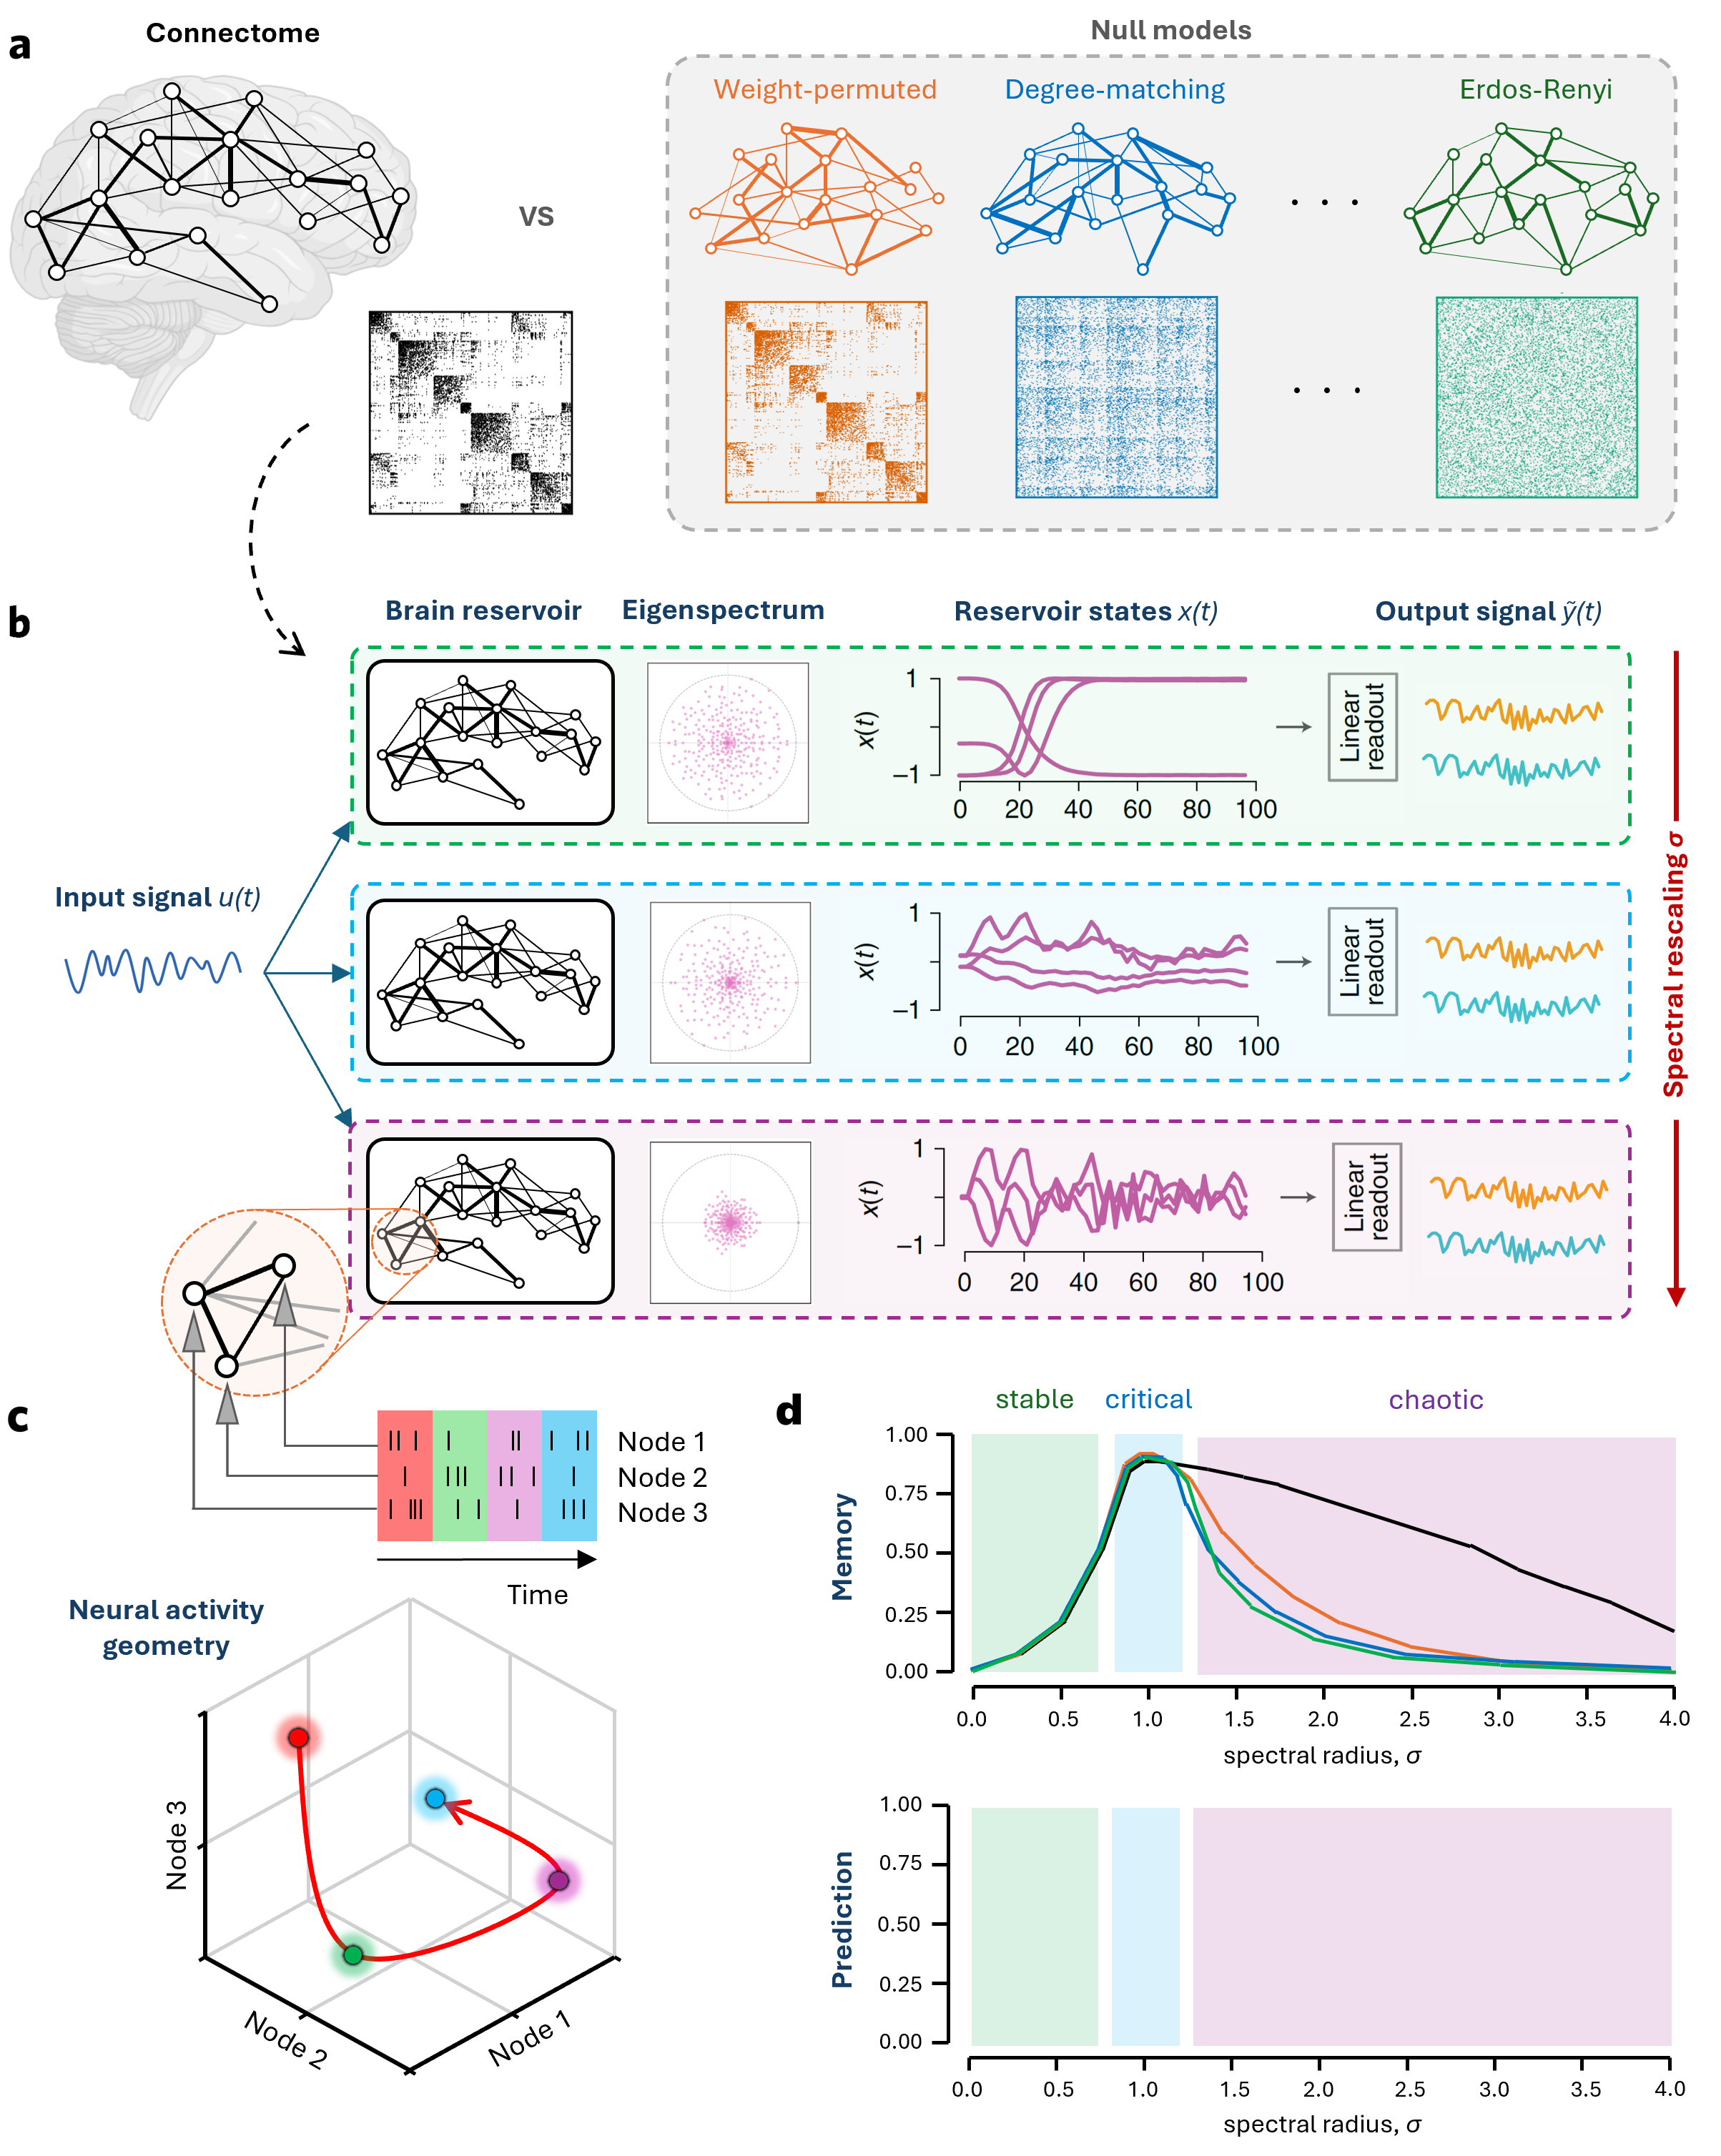
\includegraphics[width=\textwidth]{figures/Intro-Schematic.png}
    \caption[Main fig]{
    \textbf{Overview schematic:} Caption to be written soon...}
    \label{fig:project-schematic}
\end{figure}


\afterpage{\blankpage}
              
    \chapter{Background \& Related Work}
\label{chapter:literature-review}


% Connectomics and Network Neuroscience
\section{No Neuron Is an Island}
\label{section:ch1_1}


% Human Connectome image
\begin{figure}[ht]
    \centering
    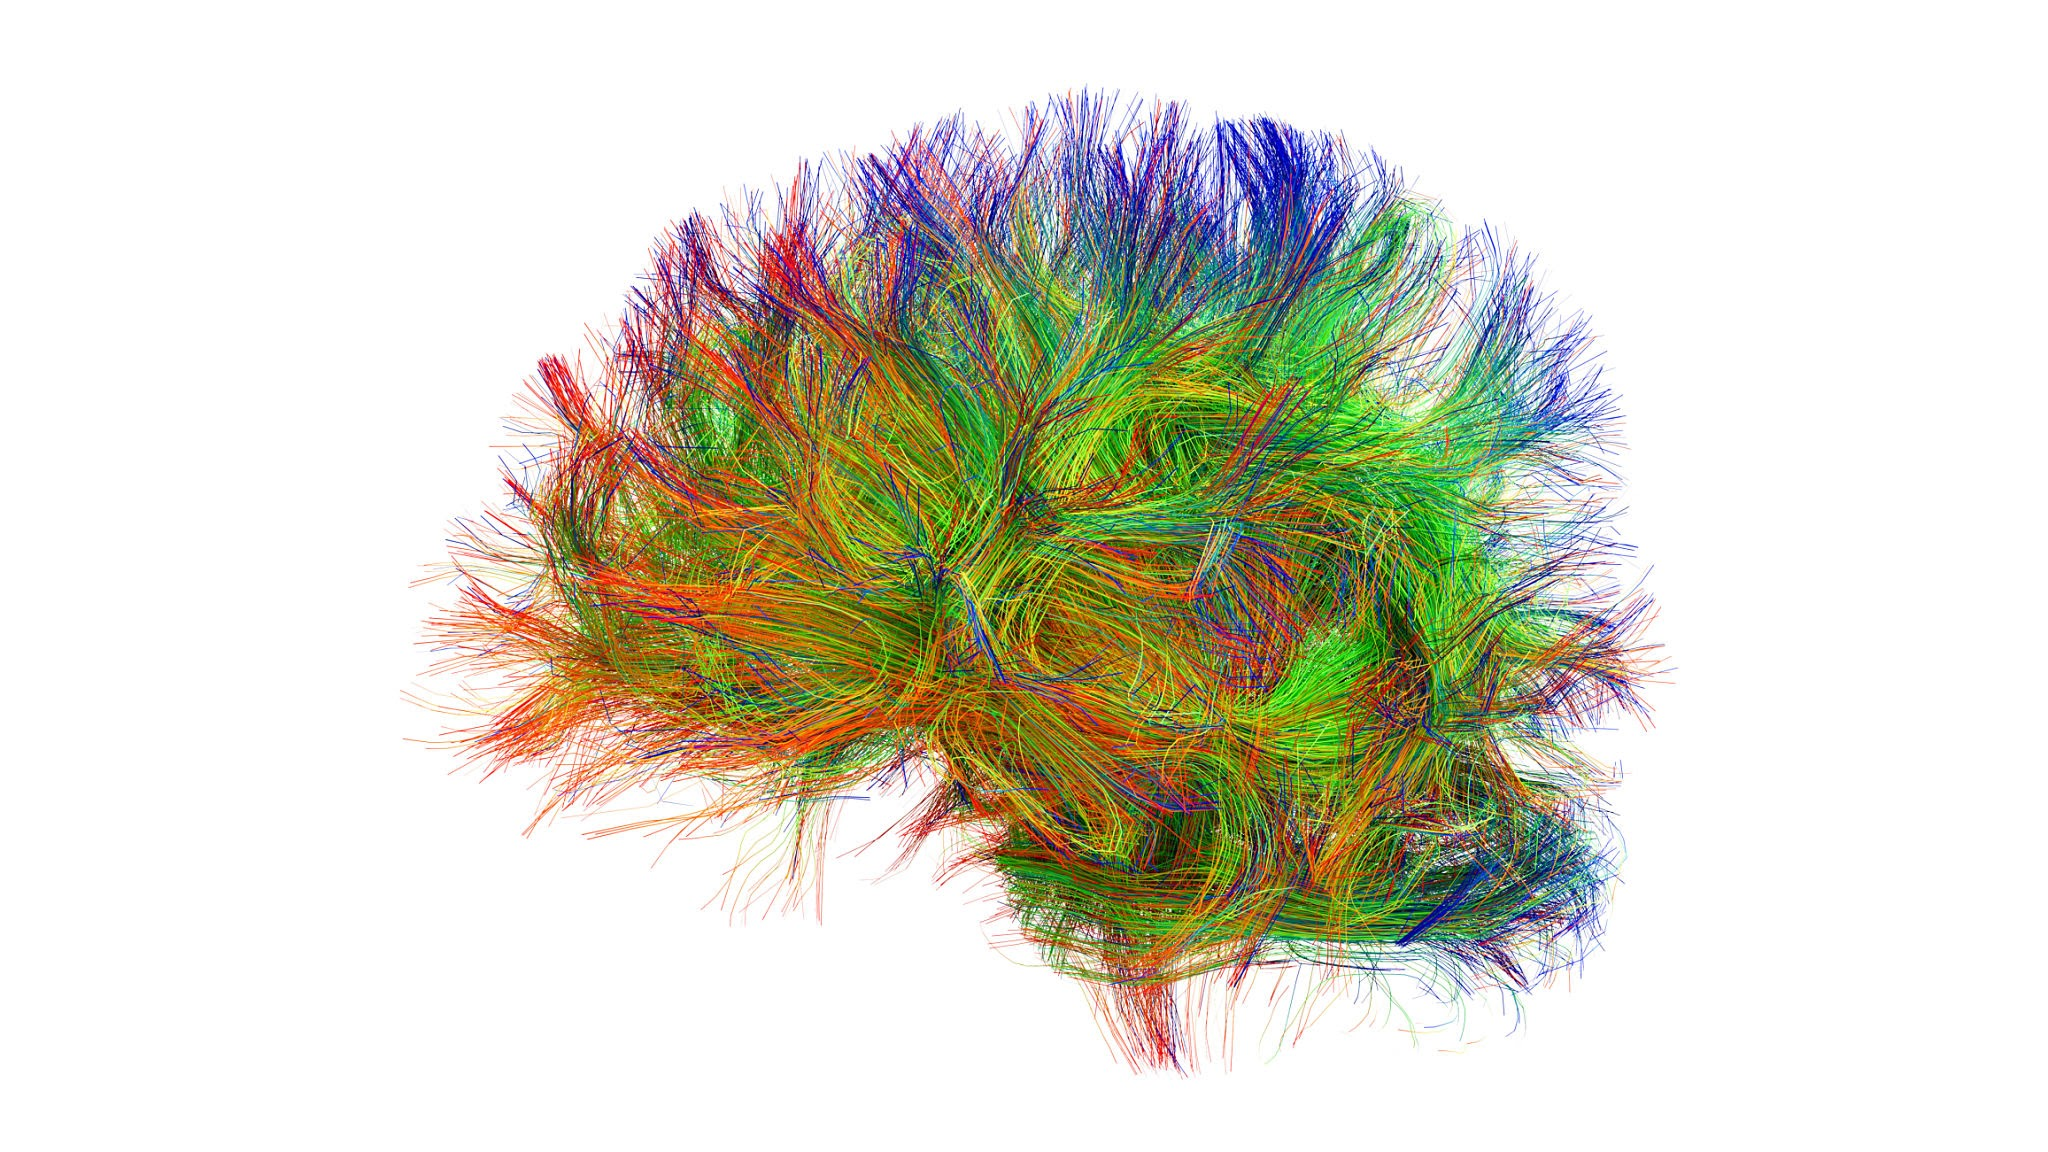
\includegraphics[width=\textwidth]{figures/Human_connectome.jpg}
    \caption[Human Connectome]{\textbf{The human structural connectome}}
    \label{fig:human-connectome}
\end{figure}



% Spectral Graph Theory
\section{The Value of Eigenvalues}
\label{section:ch1_2}

% Perron-Frobenius Theory


% Neural population dynamics and latent manifolds
\section{Dynamics on The Manifold}
\label{section:ch1_3}


% Connectome-constrained networks
\section{Wiring Dictates Firing}
\label{section:ch1_4}


% Reservoir Computing Models
\section{Models of The Mind}
\label{section:ch1_5}


   
    \chapter{Methods}
\label{chapter:methods}


\section{Reservoir computing}

\section{Connectivity substrates}

% Constructing a group concensus network

\section{Network null models}

\section{Computational tasks}

\subsection{Memory capacity}
\subsection{Dynamical systems}

\section{Measures}

 
    \chapter{Structure Sets the Spectrum}
\label{chapter:act-I}

% Chapter 4 opening:

Chapter~\ref{chapter:prelims} divided the spectrum of a connectivity matrix into
two parts with different roles. The leading eigenvalue sets the gain, and with it
the dynamical regime the network occupies; it is the part we rescale and
therefore the part we control. The eigenvalues beneath it are where a particular
wiring leaves its mark. That division was introduced as a way of reading a
spectrum. This chapter measures it, on a human connectome and on a family of
substrates that destroy parts of its organisation one at a time. Nothing here is
simulated. Every quantity reported is computed from the connectivity matrix
alone, before any input is presented, which is what makes the spectrum the first
link in the chain and the only one that can be examined without running the
network at all.

What separates a connectome from a randomised network of the same size is not
the bulk. Measured in the raw units of the weights, the bulk edges of the
connectome and of every substrate tested against it agree to within a few per
cent. What separates them is the outlier. The connectome's leading eigenvalue
stands more than three times clear of its own bulk edge, where every other
substrate stands under two, and essentially the whole difference between them
sits in that one number. This is worth stating carefully, because the convention
in this literature is to divide each matrix by its own leading eigenvalue before
comparing, and in those units the connectome's bulk is the narrow one. That
narrowness is a property of the divisor rather than of the bulk, and the divisor
is the one quantity the substrates differ in. Stated in the direction the
measurement supports, the connectome's weight assignment buys a large spectral
gap rather than a compact bulk.

The assignment is the operative object, and not the graph or the weights taken
separately. A control that holds the connectome's own edge set and its own
weights and reshuffles only which edge carries which value lands with the
randomised substrates rather than with the connectome. No measure of the binary
graph distinguishes the two, and no statistic of the weight values distinguishes
them either, since the multiset is identical. Neither is sufficient on its own.
What produces the gap is the correspondence between them.

That localises the effect without explaining it. Which property of the
assignment is responsible remains open, and the one candidate specific enough to
test here, a weighted rich club in which the heaviest edges run between the
highest-degree parcels, is ruled out by the measurement. A spectrum also says
nothing about what a network does with what it is given. It describes an
operator, and where each part of that operator ends up in the activity the
operator generates is the question of Chapter~\ref{chapter:act-II}. Two things 
leave this chapter for it. The first is a scale that every substrate carries with 
it, the point at which its own bulk edge reaches one; it makes a second way of 
matching substrates possible, and the closing section sets out why neither way is 
neutral. The second is a mode standing clear of the bulk, handed on as an object 
to be decomposed rather than as an explanation.






\section{The substrate and its null ladder}
\label{sec:act1-substrate}
\bigskip

The substrate is a human structural connectome at 448 cortical
parcels, % METH A.4
built for this thesis as a group consensus over the diffusion-weighted scans of
a publicly released healthy-adult cohort \cite{griffa2019structural,
suarez2021learning} rather than taken from a published matrix. Two of its
properties carry through the whole thesis. It is symmetric, and therefore
normal, which fixes the form its spectrum can take. And it is non-negative,
since tractography counts streamlines and cannot represent an inhibitory
connection. The same build at
$N = 1000$ % METH A.4
supports the change of scale in Section~\ref{sec:act1-scale}. Construction is in
Chapter~\ref{chapter:methods}.

Against the connectome stand three randomised substrates, each destroying some
part of its organisation and holding the rest fixed.
Table~\ref{tab:act1-preservation} sets out what each keeps, and
Figure~\ref{fig:F19} shows what that looks like as a graph. An Erdős–Rényi
graph matches the node count, edge count and density exactly rather than in
expectation, and panel~(d) is the result: connections scattered uniformly, with
none of the block structure of panel~(a). A degree-preserving rewire adds the
degree sequence, so it carries the connectome's heavy-tailed degree
distribution intact, visible in the marginal above panel~(c), while the blocks
go the same way. Weights are painted onto both by drawing, with replacement,
from the connectome's own multiset of edge
weights, % METH B.0
so the ladder varies where weight sits without changing what weights are
available.

The third randomised substrate is not a null but a control. The weight-permuted
variant takes the connectome's own graph and its own weights and permutes the
weights across the edges, and panels~(a) and~(b) of Figure~\ref{fig:F19} are the
same image because of it: same edge set, same degrees, and the same weight
multiset exactly rather than in distribution, since the values are reordered
rather than resampled. % METH B.1
The magnified block below makes the one difference legible. In (i) and (j) the
same cells are filled and the colours in them are not the same colours. No
measure of the binary graph separates the two substrates, which is what
Table~\ref{tab:act1-topology} reports: identical clustering, identical
modularity on a fixed partition, identical assortativity and identical
efficiency, as any such measure must return on one graph. Against the
connectome the control isolates weight assignment, holding topology and weight
statistics fixed together; against the degree-preserving rewire it isolates
topology, since the two draw their weights from the same pool and differ in the
graph. Each of the three randomised substrates is generated at ten
seeds; % METH B.0
the connectome is one fixed graph and returns the same matrix every time. 
Three further substrates are not among the four drawn here and are described 
in Chapter~\ref{chapter:methods}; Figure~\ref{fig:S4} draws the whole family
together and their spectra are in Appendix~\ref{app:wider-ladder}.


% Null model preservation table, four drawn rungs only.
\begin{table}[ht]
    \centering
    \caption[What each substrate preserves]{\textbf{What each substrate
    preserves and what it destroys.} The four substrates the figures of this
    chapter draw, ordered by how much of the connectome each keeps, most at the
    top. All four share the connectome's node count, edge count, density and
    non-negative weights, so those properties are not columns here; what
    separates them is everything below that. The weight-permuted variant is a
    control rather than a null, preserving the graph entire and destroying only
    the assignment of weights to edges. Generation procedures, and the three
    further substrates this chapter does not draw, are in
    Chapter~\ref{chapter:methods}.}
    \label{tab:act1-preservation}
    \begin{tabular}{lcccc}
        \toprule
        & degree & clustering & modularity & weight \\
        & sequence &  &  & assignment \\
        \midrule
        \textbf{connectome} & \checkmark & \checkmark & \checkmark & \checkmark \\
        weight-permuted & \checkmark & \checkmark & \checkmark & --- \\
        degree rewire & \checkmark & --- & --- & --- \\
        Erdős–Rényi & --- & --- & --- & --- \\
        \bottomrule
    \end{tabular}
\end{table}

% Four Substrates Adjacency Matrices Figure
\begin{figure}[htbp]
    \centering
    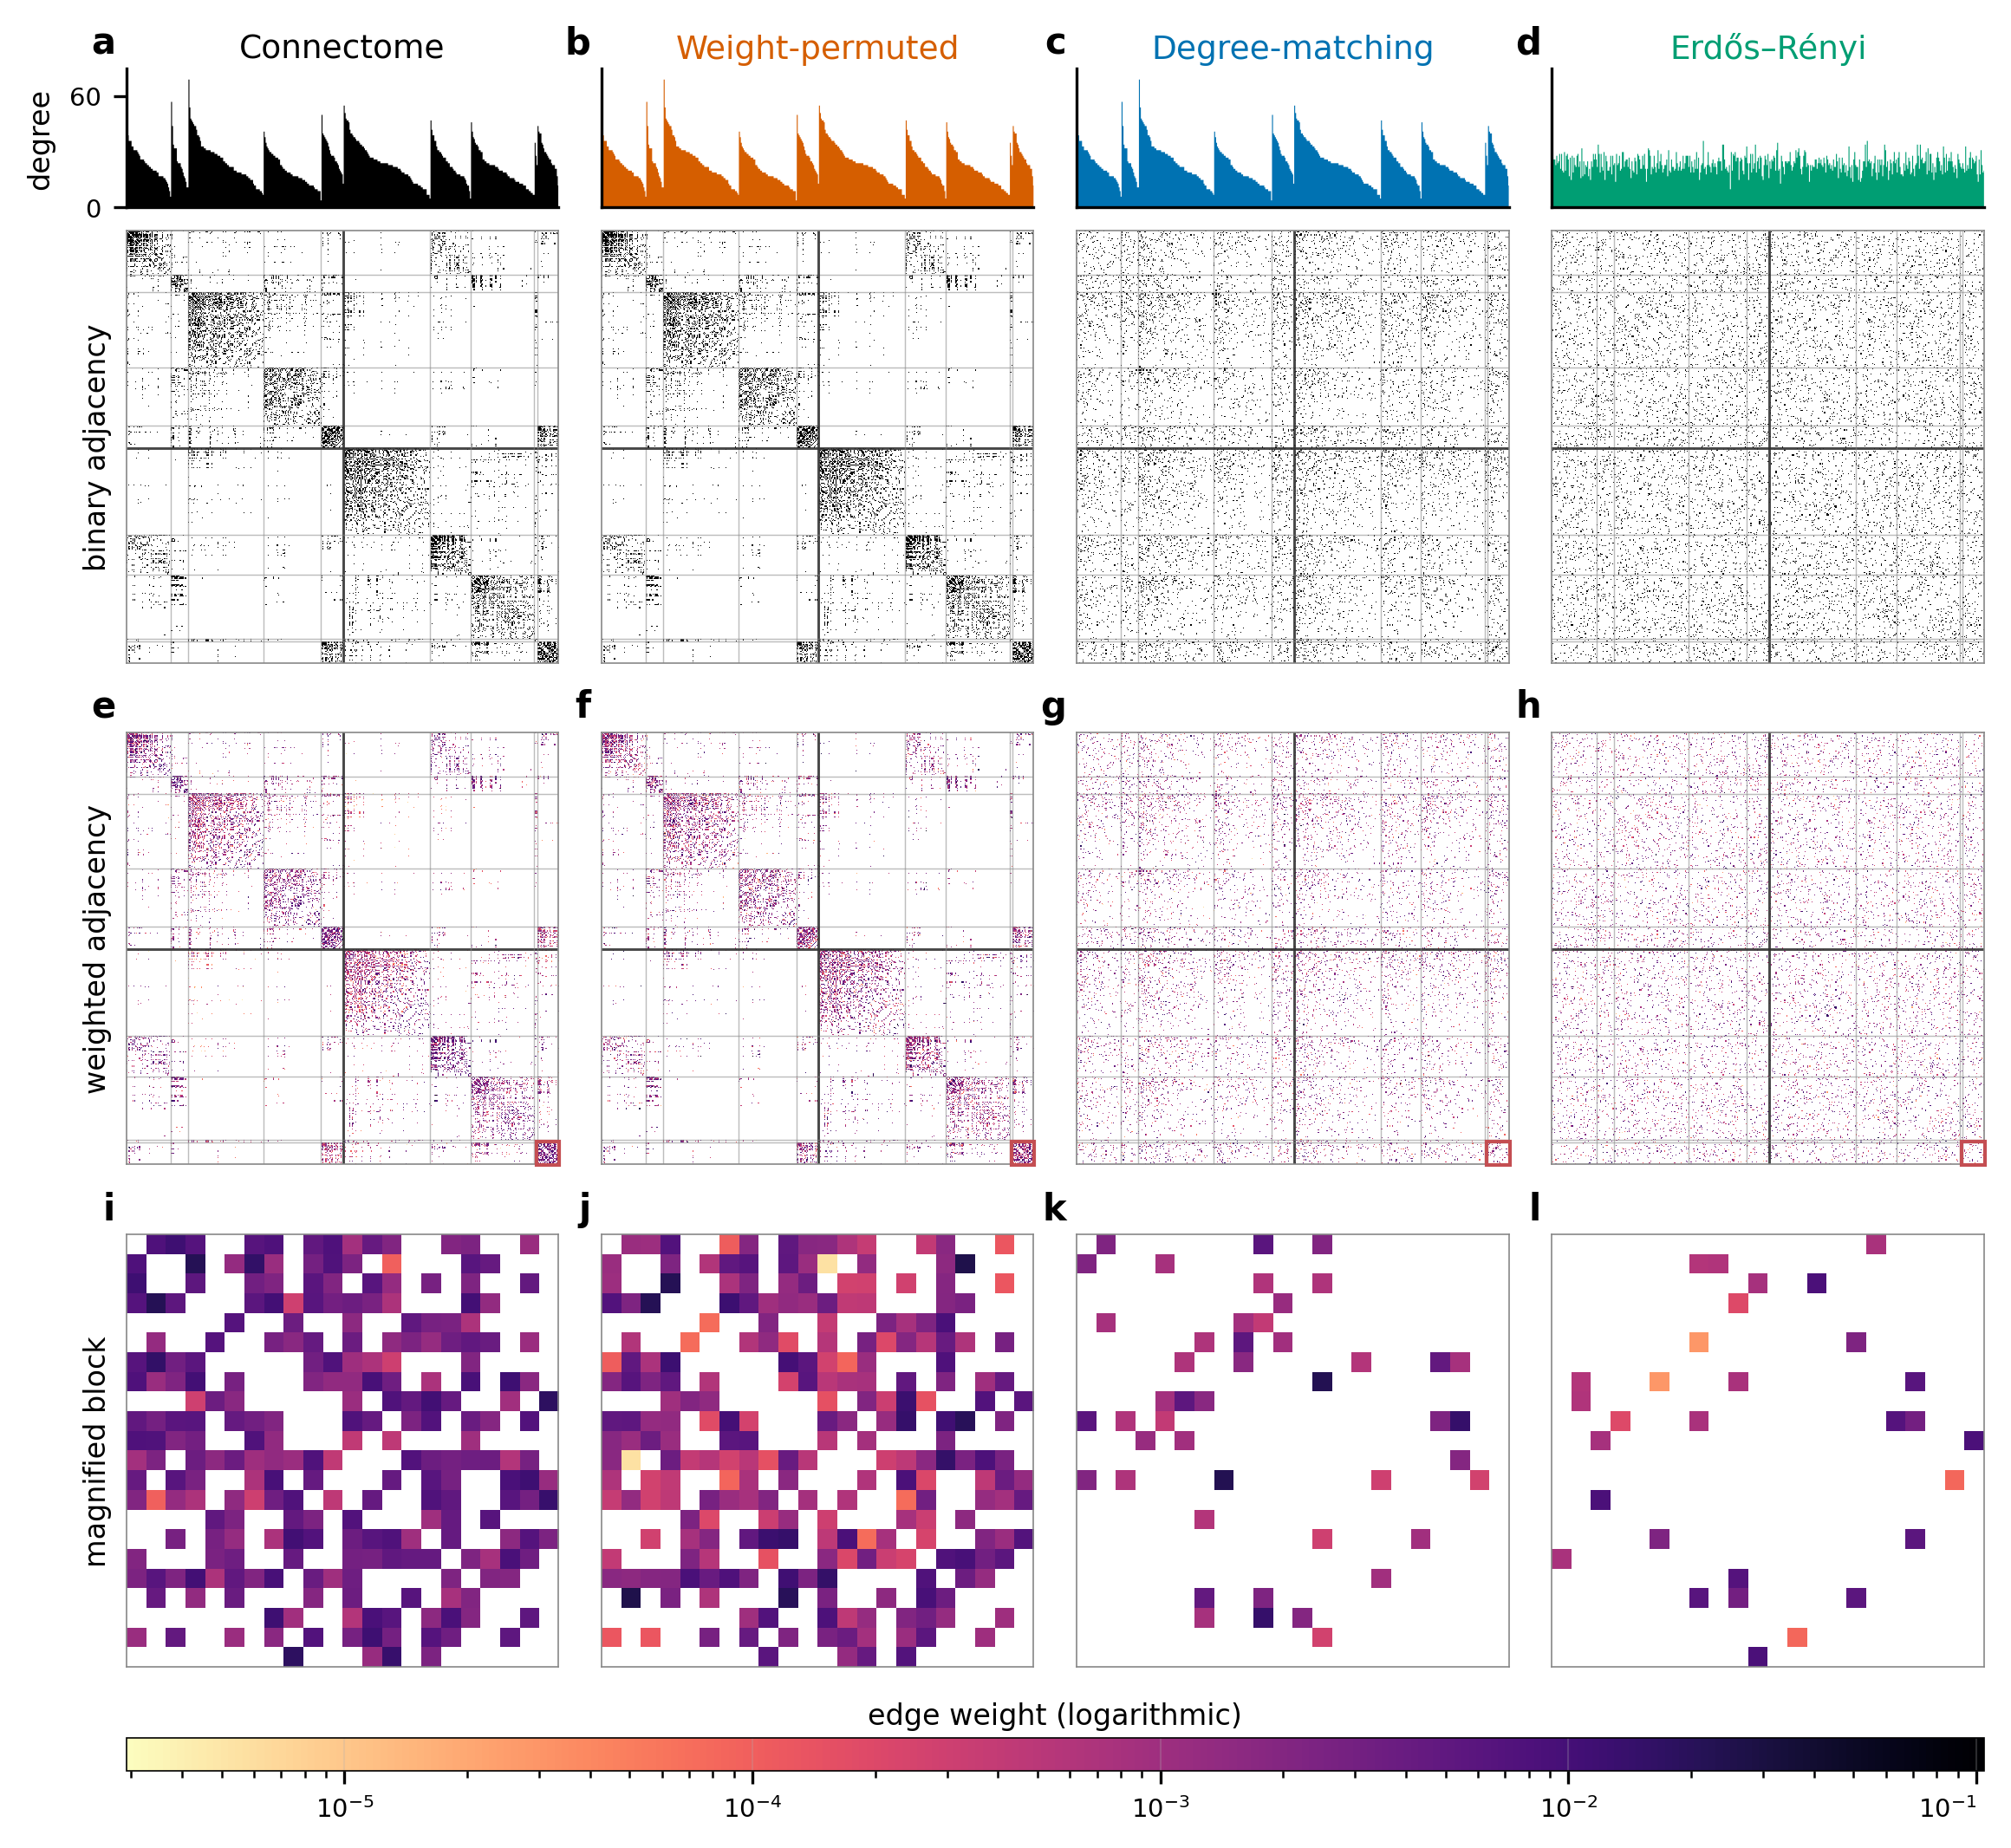
\includegraphics[width=\textwidth]{F19.png}
    \caption[The four substrates, as graphs]{%
    \textbf{No measure of the binary graph separates the connectome from its
    control.} The four substrates of this chapter, drawn under one node
    ordering: hemisphere, then community, with communities detected once on the
    connectome and reused for every panel. All four hold
    448 % METH A.4
    nodes and 5{,}323 % METH A.6
    undirected edges at a density of 5.32\% % METH A.6
    by construction. \textbf{(a--d)} Binary adjacency, with the degree marginal
    above each panel. Panels (a) and (b) are the same image: the
    weight-permuted control preserves the connectome's edge set exactly, so the
    two are one graph. The degree-preserving rewire (c) keeps the marginal and
    loses the block structure; Erdős–Rényi (d) keeps neither. \textbf{(e--h)}
    Weighted adjacency on a shared logarithmic colour scale, same ordering.
    \textbf{(i--l)} One diagonal block magnified, marked on (e--h) and drawn on
    the same colour scale: one hemisphere's share of one community, the densest
    such block of between 15 and 40 nodes. % TIER0 3.13
    In (i) and (j) the same cells are
    filled, because the edge set is the same edge set; what the permutation
    changes is which weight sits in each of them, drawn from the whole graph's
    multiset rather than from this block's. The same nodes in (k) and (l) form
    no block at all. Randomised substrates are drawn at the seed used
    throughout this chapter. Topology statistics are in
    Table~\ref{tab:act1-topology}; where these substrates differ is the
    spectrum, in Section~\ref{sec:act1-spectrum}.}
    \label{fig:F19}
\end{figure}

% Topology comparison table
\begin{table}[ht]
    \centering
    \caption[Topology of the four substrates]{\textbf{Topology of the four
    drawn substrates.} All four statistics are measures of the binary graph,
    weights discarded; medians over ten seeds for the two randomised
    substrates, which are single values for the connectome and its control.
    Modularity is evaluated on one partition, detected once on the connectome
    and applied unchanged to all four, so the four scores are comparable;
    detecting communities separately would find them in Erdős–Rényi too. The
    connectome and the weight-permuted control return identical values on every
    statistic, as any measure of the binary graph must, since they are the same
    graph. Rows are ordered as in Table~\ref{tab:act1-preservation}.}
    \label{tab:act1-topology}
    \begin{tabular}{lrrrr}
        \toprule
        & mean & modularity & degree & global \\
        substrate & clustering & (fixed part.) & assortativity & efficiency \\
        \midrule
        \textbf{connectome} & 0.4277 & 0.5486 & 0.1067 & 0.4064 \\ % TIER0 3.13
        weight-permuted & 0.4277 & 0.5486 & 0.1067 & 0.4064 \\ % TIER0 3.13
        degree-preserving rewire & 0.0697 & $-0.0002$ & $-0.0192$ & 0.4789 \\ % TIER0 3.13
        Erdős–Rényi & 0.0529 & $-0.0036$ & $-0.0068$ & 0.4820 \\ % TIER0 3.13
        \bottomrule
    \end{tabular}
\end{table}



\section{An outlier and a bulk}
\label{sec:act1-spectrum}
\bigskip
% Outline items 3 and 4. Carries A1.1, A1.2, A1.3. Figures F1, F2.

The connectome's spectrum is a dense band about the origin and one eigenvalue
standing well clear of it at the right-hand edge, which is panel~(a) of
Figure~\ref{fig:F1}. It is also entirely real, as symmetry requires, and not
merely to within a tolerance one could work with: across all forty ladder cells
at $N = 448$ the largest imaginary part in the stored spectra is exactly
zero, % A1 2.5
and the symmetry check holds in every row. % A1 2.5
Figure~\ref{fig:F1} is therefore drawn on the real line rather than in the
complex plane, where a second dimension would carry nothing.

The separation itself is guaranteed rather than an accident of this particular
graph. Non-negativity gives $W$ a real, positive leading eigenvalue, largest in
modulus and with a non-negative eigenvector, and the only question a given
substrate answers is how far clear of everything else that eigenvalue sits.
Three terms follow. The \emph{Perron root} $\lambda_1$ is that leading
eigenvalue, the \emph{bulk} is the band holding the remainder, and the
\emph{gap} is the separation between them. Measuring the gap needs an edge for
the bulk, and the one used throughout is $\mathrm{bulk95}$, the 95th percentile
of $|\lambda|$ over the spectrum as a fraction of
$\lambda_1$. % A1 2.6 finding 1
All three are properties of a single substrate, measured before any comparison
is made.

\begin{figure}[htbp]
    \centering
    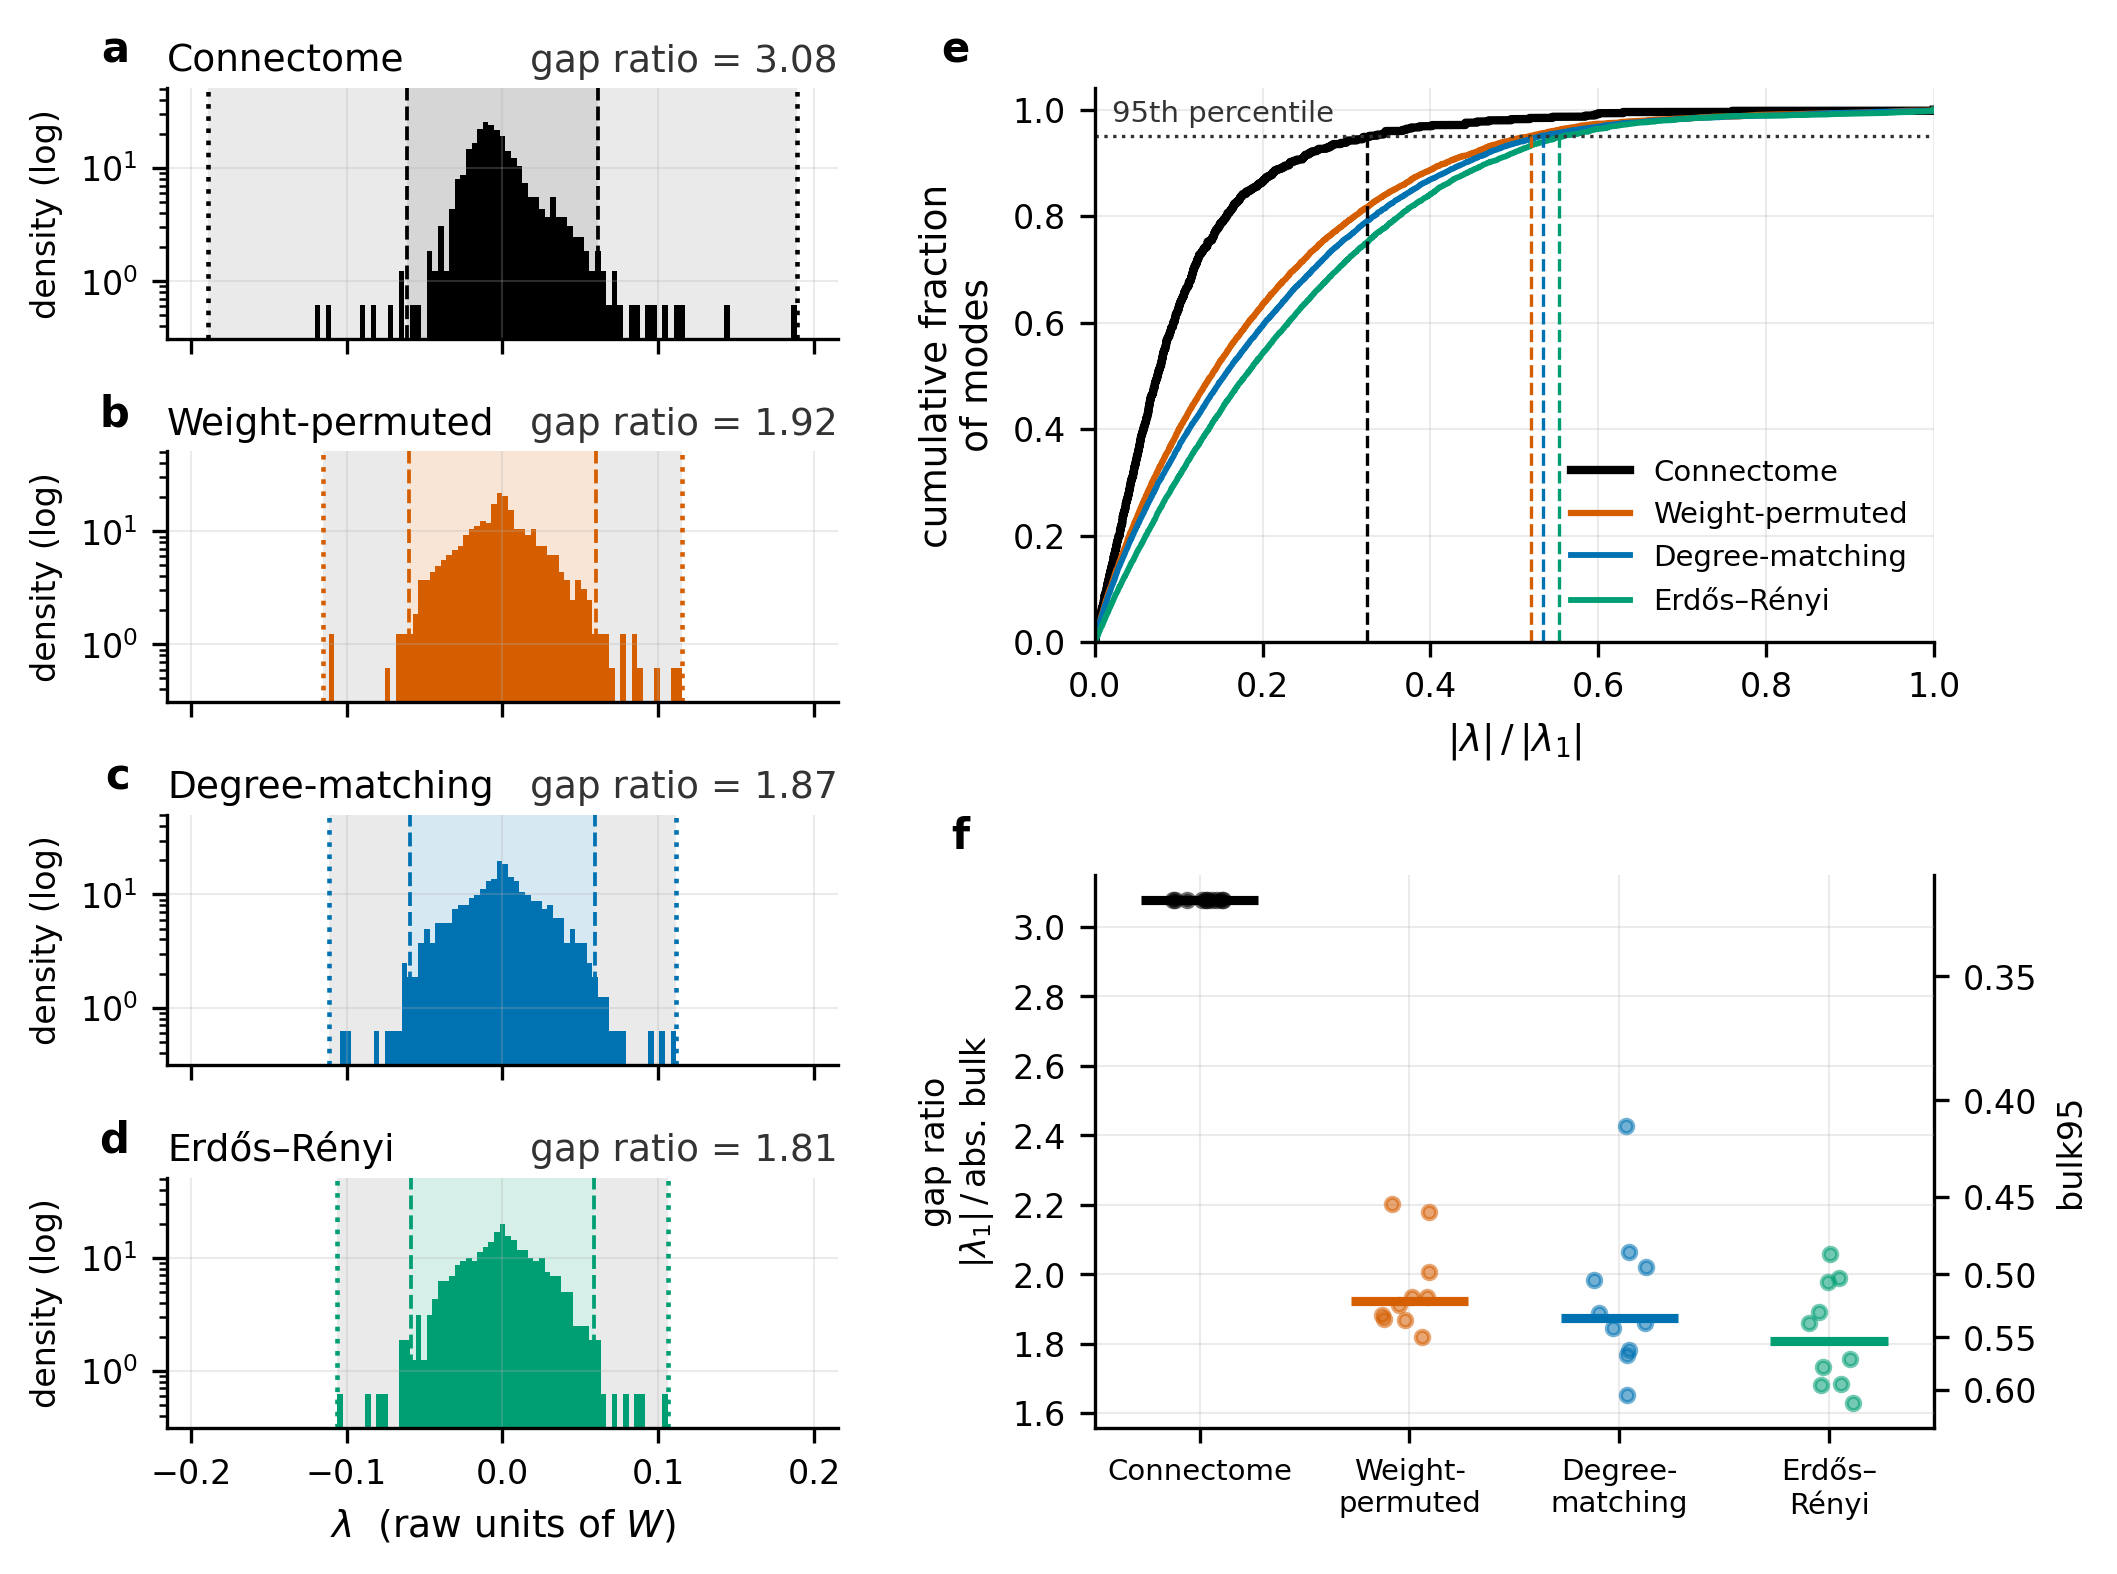
\includegraphics[width=\textwidth]{F1.png}
    \caption[The connectome's weight assignment buys a large spectral gap]{%
    \textbf{The connectome's weight assignment buys a large spectral gap.} Eigenvalues of the un-rescaled recurrent matrix $W$ on the
    all-positive human substrate ($N = 448$ % TIER0 2.1
    self-built consensus, empirical weights).
    \textbf{(a--d)} One substrate per row, raw units, shared axis: the bulk
    shaded to $\pm$ the absolute bulk radius, the gap out to $\pm\lambda_1$ in
    grey. Sighting down the column, the four bulk edges hold while $\lambda_1$
    (dotted) separates and the grey gap grows from row d to row a; the
    weight-permuted control (b) sits with the nulls. Each row draws one
    spectrum, for the nulls the seed whose $\mathrm{bulk95}$ is nearest the
    median, so all four carry equal sampling noise. \textbf{(e)} The same
    spectra as cumulative distributions, each divided by its own $\lambda_1$,
    the normalisation the connectome-reservoir literature uses, and every nominal 
    spectral-radius-matched comparison in this thesis with it.
    The curves separate everywhere; the 95\% crossings are
    $\mathrm{bulk95}$ itself. \textbf{(f)} The gap ratio per seed, with
    $\mathrm{bulk95}$ on the right-hand axis. The connectome's ten seeds
    coincide exactly.}
    \label{fig:F1}
\end{figure}

The connectome's Perron root stands
more than three % (3.078) TIER0 3.1
times clear of its own bulk edge at $N = 448$. % TIER0 3.1
Every other substrate the figures draw stands between
1.81 % TIER0 3.1
and 1.92 % TIER0 3.1
times clear of its own. That ratio, the Perron root over the absolute bulk
radius, is the gap ratio, and the connectome's is at least
1.6-fold % TIER0 3.1(b)
above every rung of the four-substrate ladder it is measured against. The gap is
not bought by a narrower bulk. It is bought by a higher outlier over a bulk that
is essentially everyone's.

Figure~\ref{fig:F1} draws the eigenvalues of the un-rescaled matrix $W$, one
substrate per row, on a shared axis in the raw units of the weights, and the
first thing to do with it is to sight down the column. The four bulk bands sit
at the same place. Their edges fall between
0.0587 % TIER0 3.1
and 0.0614, % TIER0 3.1
a spread of 4.4\% % TIER0 3.1
of their mean at $N = 448$. % TIER0 3.1
What moves is the outlier. The Perron root runs from
0.1061 % TIER0 3.1
at the Erdős–Rényi rung to 0.1889 % TIER0 3.1
at the connectome, so the grey region separating the bulk from $\lambda_1$ grows
steadily up the column while the coloured band beneath it stays put.
Figure~\ref{fig:F2} makes the same decomposition as medians across the ladder,
the absolute bulk in panel~(a) and the Perron root in panel~(b), and
Table~\ref{tab:act1-ladder} gives the values at both parcellations.

Reported instead as a fraction of each substrate's own Perron root, those same
four bulk radii spread 47.3\%. % TIER0 3.1
Nothing about the bulks has moved between those two numbers. Only the divisor
has. Panel~(e) is where the divisor becomes visible: it redraws the same spectra
as cumulative distributions after each substrate has been divided by its own
$|\lambda_1|$, the normalisation every spectral-radius-matched comparison in the
connectome-reservoir literature
uses \cite{suarez2021learning, suarez2024connectome, milisav2026neuromorphic}.
In those units the curves separate everywhere and the connectome's reads as the
narrow one, with $\mathrm{bulk95}$ legible at the crossings of the 95\% level.
Read that way, the connectome has an anomalously compact bulk.
Read in the units of the weights it has nothing of the kind: the four bulks
agree, and what the connectome has instead is a Perron root
1.78 % TIER0 3.1
times the Erdős–Rényi rung's. % TIER0 3.1(a)
The two halves of the figure are the same spectra one division apart, and the
compactness belongs to the divisor. Stated in the direction the measurement
supports, the difference is an anomalously large spectral gap.

The ratio has two other names, and all three are the same number:
$|\lambda_1| / \mathrm{abs\_bulk} = 1/\mathrm{bulk95} = \mathrm{sr\_crit}$. % TIER0 3.1
The gap ratio, the inverse bulk and the critical scale are one quantity, which
is why panel~(f) can carry $\mathrm{bulk95}$ on its right-hand axis, and why the
name $\mathrm{sr\_crit}$ is the one worth adopting: it names the quantity after
what it measures, the nominal spectral radius at which the median seed's bulk
edge reaches one.\footnote{The edge in question is the 95th percentile of
$|\lambda|$, % A1 2.6 finding 1
so at $\sigma = \mathrm{sr\_crit}$ five per cent % A1 2.6 finding 1
of modes already exceed unity. $\mathrm{sr\_crit}$ is a criticality scale each
substrate carries with it, not the point at which that substrate becomes
supercritical. Chapter~\ref{chapter:methods} gives the aggregation the identity
holds under.}

\begin{table}[ht]
    \centering
    \caption[The substrate ladder at both scales]{\textbf{The substrate ladder
    at both scales.} Medians over ten seeds; the connectome is one fixed graph,
    so its seeds coincide exactly and only the nulls are resampled.
    $|\lambda_1|$ and the absolute bulk radius are in raw units of $W$; the
    absolute bulk is the product of the medians,
    $\mathrm{median}(\mathrm{bulk95}) \times \mathrm{median}(|\lambda_1|)$, and
    $\mathrm{bulk95}$ is the ratio of the two. Spread is the range over the
    mean. The entire between-variant difference sits in $|\lambda_1|$, which is
    why the two spreads differ by close to an order of magnitude. 
    Rows are ordered as in Table~\ref{tab:act1-preservation} rather than by value; 
    the gap-ratio column is not monotone at $N = 1000$.}
    \label{tab:act1-ladder}
    \begin{tabular}{lrrrr}
        \toprule
        substrate & absolute bulk & $|\lambda_1|$ & $\mathrm{bulk95}$ & gap ratio \\
        \midrule
        \multicolumn{5}{l}{\emph{$N = 448$}} \\
        connectome & 0.0614 & 0.1889 & 0.3249 & \textbf{3.078} \\ % TIER0 3.1
        weight-permuted & 0.0599 & 0.1152 & 0.5203 & 1.922 \\ % TIER0 3.1
        degree-preserving rewire & 0.0595 & 0.1115 & 0.5338 & 1.873 \\ % TIER0 3.1
        Erdős–Rényi & 0.0587 & 0.1061 & 0.5535 & 1.807 \\ % TIER0 3.1
        \addlinespace
        spread (range / mean) & 4.4\% & --- & 47.3\% & --- \\ % TIER0 3.1
        \midrule
        \multicolumn{5}{l}{\emph{$N = 1000$}} \\
        connectome & 0.0585 & 0.2333 & 0.2509 & \textbf{3.985} \\ % TIER0 3.1(a)
        weight-permuted & 0.0584 & 0.1398 & 0.4176 & 2.395 \\ % TIER0 3.1(a)
        degree-preserving rewire & 0.0590 & 0.1358 & 0.4346 & 2.301 \\ % TIER0 3.1(a)
        Erdős–Rényi & 0.0553 & 0.1348 & 0.4102 & 2.438 \\ % TIER0 3.1(a)
        \addlinespace
        spread (range / mean) & 6.4\% & --- & 48.5\% & --- \\ % TIER0 3.1
        \bottomrule
    \end{tabular}
\end{table}


%%%%%%%%%%%%%%%%%%%%%%%%%%%%%%%%%%%%%%%%%%%%


\section{Weight assignment and the gap}
\label{sec:act1-assignment}
\bigskip
% Outline item 5. Carries A1.5. Figure F1 (row b), Table 4.3.

What produces the gap is settled by the second row of Figure~\ref{fig:F1}. The
weight-permuted control differs from the connectome in nothing but which edge
carries which weight, and it lands with the nulls, at a gap ratio of
1.92 % TIER0 3.1
against the connectome's 3.08. % TIER0 3.1
The graph is held entire and the weight multiset is held exactly, so neither is
sufficient on its own. What buys the gap is the correspondence between them.

Two further rungs corroborate this without carrying it. Each holds more of the
connectome's topology fixed than the degree-preserving rewire does, one
preserving its community structure and one its clustering, and neither recovers
the gap; their gap ratios at both parcellations, and the margin over all six, 
are in Appendix~\ref{app:wider-ladder}. Each of those rungs fixes one
topological statistic. The control fixes the entire graph, which is why the
contrast that settles the question is the one against it.

The contrast localises the effect to the assignment. It does not say which
property of the assignment is responsible, and no mechanism is proposed for why
the assignment raises the Perron root. One account is specific enough to test on
these substrates. In a weighted rich club the heavy edges run between the
high-degree nodes, so they share endpoints and reinforce one another in the
leading eigenvalue, and a weight permutation destroys exactly that arrangement.
The prediction was registered before the measurement and it fails: edge weight
and endpoint degree product correlate at
$-0.124$ % TIER0 3.14
in the connectome, negative rather than positive and with a bootstrap interval
excluding zero, while the control sits at zero as its construction
requires. % TIER0 3.14
The connectome's heavy edges run between its lower-degree parcels, not between
its hubs, so whatever the assignment is doing to the Perron root, it is not
assembling a heavily weighted core. Appendix~\ref{app:mechanism} gives the test,
its two other predictions, and the account left standing by it, which is not
tested here.


%%%%%%%%%%%%%%%%%%%%%%%%%%%%%%%%%%%%%%%%%%%%


\section{The gap across scale}
\label{sec:act1-scale}
\bigskip
% Outline item 6. Carries A1.4. Figures F2 (both scales), S1 (appendix).

The connectome's spectral gap survives a more than two-fold
% (2.2-fold) TIER0 1.4
change in the number of nodes. The whole ladder was rebuilt at
$N = 1000$, % TIER0 2.1
and panel~(c) of Figure~\ref{fig:F2} is where that shows: the connectome's gap
ratio is 3.99 % TIER0 3.1
against 2.30 to 2.44 % TIER0 3.1
for the three rungs drawn beside it, again at least
1.63-fold % TIER0 3.1(b)
clear of every one, with the full ladder at both parcellations in
Table~\ref{tab:act1-ladder}.
Two parcellations are one step and there is no third, so
this is a robustness check across a single change of scale rather than a
demonstration of invariance.

What does not survive is the near-identity of the bulks. At $N = 448$ the four
absolute bulk radii agree to 4.4\% % TIER0 3.1
of their mean; at $N = 1000$ they spread 6.4\%, % TIER0 3.1
or 6.9\% % TIER0 3.1
if the per-seed products are taken before the median rather than after.
\emph{Near-identical} describes $N = 448$; at $N = 1000$ the right word is
\emph{close}. The loosening is narrower than the summary figure suggests, since
three of the four substrates still sit within
1.1\% % TIER0 3.1(a)
of one another and the whole of the difference is the Erdős–Rényi rung sitting
low. Scale also unsettles the ordering among the nulls, which does not hold
between the two parcellations on either the bulk edge or the absolute
bulk.\footnote{The largest absolute bulk belongs to the connectome at
$N = 448$ and to the degree-preserving rewire at
$N = 1000$. % TIER0 3.1(a)
Figure~\ref{fig:S1} rebuilds Figure~\ref{fig:F1} at the larger parcellation with
its rows in ladder order, so the gap ratios run down that column out of
sequence.} What is scale-robust is the connectome's separation from the other
three, not the coincidence of the bulks and not any arrangement among the nulls.


\begin{figure}[htbp]
    \centering
    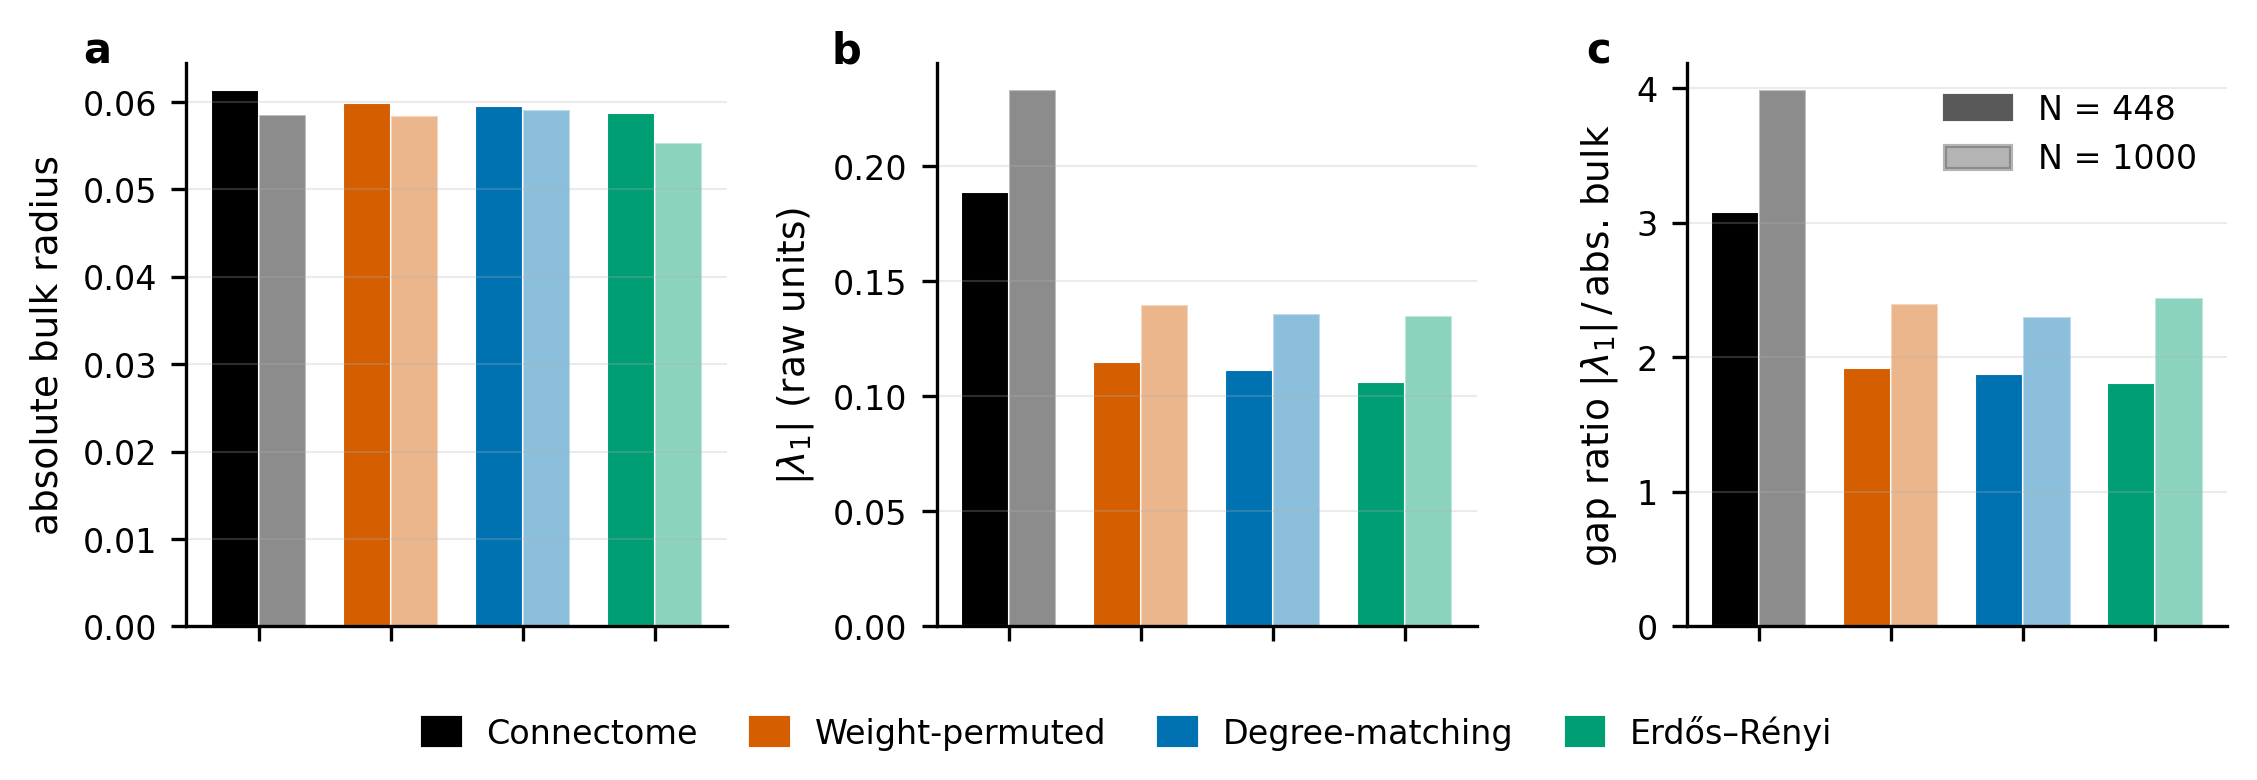
\includegraphics[width=\textwidth]{F2.png}
    \caption[The difference is a gap, and the gap is what carries across
    scale]{%
    \textbf{The difference between the connectome and its nulls is a spectral
    gap, and what carries across scale is the gap.} The four drawn substrates at
    both parcellations, ten seeds each (solid $N = 448$, % TIER0 2.1
    translucent $N = 1000$). % TIER0 2.1
    All three panels are zero-based and use one aggregation throughout, the
    median over seeds of $\mathrm{bulk95}$ and of $|\lambda_1|$, so (c) is
    exactly (b) divided by (a). \textbf{(a)} The absolute bulk radius,
    near-identical across the four at $N = 448$ and merely close at $N = 1000$.
    \textbf{(b)} $|\lambda_1|$ in raw units, where the substrates do separate.
    \textbf{(c)} The gap ratio, identically
    $1/\mathrm{median}(\mathrm{bulk95})$ and identically the critical scale
    $\mathrm{sr\_crit}$. Across a 2.2-fold % TIER0 1.4
    change in $N$ the connectome's separation from the other three holds while
    the near-identity in (a) loosens, so what is scale-robust is the separation
    and not the coincidence of the bulks.}
    \label{fig:F2}
\end{figure}




\section{What carries forward}
\label{sec:act1-handover}
\bigskip
% Outline item 7. Carries A1.6. No new measurements. Figure F3 is in
% Chapter 10; this section states the argument, not the demonstration.

The first thing to leave this chapter is $\mathrm{sr\_crit}$, the nominal
spectral radius at which a substrate's own bulk edge reaches one. Because the
gap ratio is also the inverse bulk, every substrate arrives carrying one, and
the four drawn here do not carry the same one. That is a consequence of the
result rather than a further finding, and it is what makes a second way of
matching substrates possible at all.

Comparing substrates requires putting them at the same operating point, and on
these substrates there are two ways to do it. Scaling each matrix by its own
$|\lambda_1|$ to a nominal spectral radius $\sigma$ sets the leading eigenvalue
to $\sigma$ exactly and leaves the bulk wherever it falls; this is the
normalisation the connectome-reservoir literature
uses \cite{suarez2021learning, suarez2024connectome, milisav2026neuromorphic},
and it is the one panel~(e) of Figure~\ref{fig:F1} draws. The alternative is the
product $\sigma \cdot \mathrm{bulk95}$, which holds the bulk edge fixed instead,
so that at $\sigma \cdot \mathrm{bulk95} = 1$ every substrate's bulk edge
reaches one whatever its Perron root. The second axis exists only because each
substrate carries its own $\mathrm{sr\_crit}$, which is what this chapter
supplies.

Neither axis is neutral, and the second is not a repair of the first. Each holds
fixed exactly what the other lets vary, and since these substrates differ in
essentially one quantity, no third axis holds both at once. A comparison on the
nominal axis is a comparison at matched Perron roots and unmatched bulks; one on
the matched-bulk axis is the reverse. Two consequences follow, and both are
enforced throughout what follows. Every result is quoted with the axis it was
measured on, and results on the two axes are never set against each other as
though they disagreed, because they are measurements of different things. And
the two axes cover different ranges, since holding the bulk fixed compresses the
reachable operating points by each substrate's own $\mathrm{bulk95}$: a sweep
that runs to $\sigma = 8$ on the nominal axis reaches much less far in the
matched coordinate, so a comparison there is bounded by where the substrates'
ranges still overlap, and a feature at the edge of that overlap must not be read
as though the sweep continued past it. Section~\ref{sec:methods-matching} in Methods 
shows what the choice costs on a real result.

One use of $\mathrm{sr\_crit}$ is worth flagging now, because it is a choice
rather than a consequence. The filter that separates supercritical from
subcritical operating points in Chapters~\ref{chapter:act-II}
and~\ref{chapter:act-III} is the connectome's own critical scale, applied to
every substrate rather than each substrate's own. It is the conservative
option, since it samples each null further above its own critical point than the
null's own scale would, and it is set out again where it is used.

The second thing handed on is the Perron mode. It stands clear of the bulk, and
the connectome's weight assignment is what puts it there. What the mode does is
another question, and not one a spectrum can answer: a spectrum describes an
operator, while what a network computes depends on where each part of that
operator ends up in the activity the operator generates. That is what
Chapter~\ref{chapter:act-II} measures, and the mode arrives there as an object
to be decomposed rather than as an explanation.




    \chapter{\textbf{Act II:} The Spectrum Decomposes The Activity Manifold}
\label{chapter:act-II}

\section{A critical scale, a mode, and a state matrix}
\label{sec:act2-handover}
\bigskip
% Outline item 1 (act2_manifold.md section 4). Carries no claim and points at no
% figure. One paragraph, no results: the section restates what arrives and poses
% the question. Sources: fact sheet 06. Three numerals only.
% FORBIDDEN here (sheet 06): any result; "the two axes" for sigma against f;
% "the biological cut" for f = 0; introducing f beyond the one clause below;
% "the gap keeps the Gram spectrum clear of the floor" as something Act I showed;
% "compact bulk".

% P1: the two objects received, the scope of the chapter, and the question.
Two objects arrive from Chapter~\ref{chapter:act-I}, and neither of them is a
statement about activity. The first is $\mathrm{sr\_crit}$, the nominal spectral
radius at which a substrate's own bulk edge reaches one. Because the gap ratio is
also the inverse bulk, every substrate carries its own, and the four the figures
draw do not carry the same one (Table~\ref{tab:act1-ladder}). That is what makes
the second matching axis available at all, and it is also why that axis is not
neutral: the substrates differ in one quantity only, so each axis holds fixed
exactly what the other lets vary. The second object is the Perron mode. The
previous chapter established that it stands clear of the bulk and that weight
placement is what puts it there, and it established nothing else about it, offering
no mechanism for why placement produces the gap and making no claim about capacity
or about any task. The mode arrives here as an object to be decomposed rather than
as an explanation, and that limit travels with it. Everything in this chapter sits
at the $N = 448$ % TIER0 3.12
parcellation and on non-negative weights, at $f = 0$; % SPINE, primary variable; A2 4.3.4
the sign fraction $f$ is an intervention rather than a second variable, and it
enters once, in Chapter~\ref{chapter:act-III}, where it is used to remove the
proposed cause.% TODO: repoint to the section label for 6.3 once chapter 6 exists.
The variable along which every claim below is made is the nominal spectral radius
$\sigma$, the operating point. What the reservoir's readout sees, however, is neither the
spectrum nor the operator that generates it. It is a state matrix: on the
memory-capacity task, $2500 \times 448$ % A2 2.5
real numbers, the states the reservoir passes through after its warmup is
discarded, which a ridge solver then inverts
(Chapter~\ref{chapter:methods}). So the question this chapter asks is which part
of the spectrum ends up where in the reservoir's state matrix.


\section{Three captures, and what each can be asked}
\label{sec:act2-captures}
\bigskip
% Outline item 2 (act2_manifold.md section 4). Methods. Carries no claim and
% points at no figure; it fixes definitions, operating points and scope.
% Sources: fact sheet 07, plus ACT2_CAPTURE_COVERAGE.md (tag % COV) and
% CONVENTIONS.md working rule 5 (tag % CONV).
% FORBIDDEN here (sheet 07): any ladder reading of the basis-alignment capture;
% "the manifold lives in low-frequency graph harmonics"; JUSTIFYING d_eff, which
% is section 5's; median-then-absolute-value on mean_state; "alpha was chosen at
% 1e-6 for d_eff"; "the Gram spectrum is a property of W"; "compact bulk".

% P1: the object, and the identity that poses the chapter's questions.
Everything in this chapter is measured on one object. Write the post-warmup states
as a matrix $A \in \mathbb{R}^{T_{\mathrm{eff}} \times N}$, one row per retained
timestep and one column per unit, assembled as Chapter~\ref{chapter:methods}
describes. What a linear readout can use is not $A$ itself but its second moment,
and there are two of those. The ridge solver inverts the un-centred Gram matrix
$G = A^{\top}A$; the covariance of the states about their own time-average is
formed instead from $\tilde{A} = A - \mathbf{1}m^{\top}$, where
$m = T_{\mathrm{eff}}^{-1}A^{\top}\mathbf{1}$ collects each unit's mean over time.
These are not the same object, and the difference between them is exact:
\begin{equation}
    A^{\top}A \;=\; \tilde{A}^{\top}\tilde{A} \;+\; T_{\mathrm{eff}}\,m\,m^{\top}.
    \label{eq:gram-split}
\end{equation}
Read the two terms on the right physically. The second is built from one number
per unit, the level that unit sits at on average, so it has \emph{rank one}: it
describes a single fixed pattern of activity that the network holds throughout the
run, and it says nothing about how the activity moves. The first is everything
that is left once that fixed pattern is subtracted, which is the part that varies
from one timestep to the next and therefore the only part that can carry
information about a changing input. Time-centring is the one subtraction that
separates them. The identity settles nothing on its own: it says the time-average
lives in a rank-one term, not that the Perron mode is that term, which is a
measurement and is made in Section~\ref{sec:act2-perron}.

% P2: the three questions the identity poses, and one capture per question.
Equation~\ref{eq:gram-split} poses three questions, and this chapter answers them
with three frozen captures, one apiece. \textbf{How large is the rank-one term?}
That is a question about a single scalar per run, and the
\emph{saturation-diagnostics} capture records it, along with the related quantities
describing where the units are sitting: how far the network has been driven into
the flat regions of its nonlinearity, and how strongly it has synchronised.
\textbf{What is the remaining, fluctuating term organised by?} A cloud of activity
in $N$ dimensions can be described in any orthonormal coordinate system, and asking
which one lines up with the fluctuations is asking which structural feature of the
network they follow. The \emph{basis-alignment} capture answers it by projecting
the time-centred states onto the leading $k$ vectors of three candidate bases and
recording the fraction of variance each holds: the eigenvectors of $W$, so the
dynamical modes themselves; the low-frequency harmonics of the graph Laplacian,
which are the smoothest patterns the wiring supports and are the network's
analogue of low-frequency Fourier modes \cite{atasoy2016human}; and a random orthonormal basis, which
supplies the chance level, since $k$ arbitrary directions out of $N$ capture about
$k/N$ of the variance by construction and a basis that fails to beat that has told
us nothing. \textbf{And how many directions of the fluctuating term does the
readout actually have available?} That is set by where the eigenvalues of $G$ sit
relative to the regularisation, so the \emph{Gram-spectra} capture stores the whole
spectrum, all $N$ eigenvalues per run, rather than any summary of it. Storing the
spectrum rather than the states is deliberate and is what makes the later sections
possible: a state matrix runs to tens of megabytes per cell where a spectrum is
$N$ floating-point numbers, % CONV working rule 5
and every dimensionality measure this chapter uses is a function of the spectrum
alone, so it can be recomputed afterwards at any regularisation strength without
re-running anything.

% P3: the scope limit on the narrowest capture, and the supercritical filter.
The basis-alignment capture is much the narrowest of the three, and its limits are
stated here rather than in a limitations section because they bind every sentence
drawn from it. It holds two substrates, the connectome and the degree-preserving
rewire, % COV 3.1
and each weight condition was captured at two spectral radii only: one low point
shared across conditions and one higher point of its own, which for the
all-positive weights used throughout this chapter is
3.0526. % COV 3.4
So nothing drawn from it may be read as a result about the null ladder, since it
carries neither an Erdős–Rényi rung nor the weight-permuted control, and the panels
of Figure~\ref{fig:F5} each sit at their own condition's operating point rather
than at one shared radius. Where anything below is called \emph{supercritical} it
means a nominal spectral radius of at least
3.05, % TIER0 3.2
the connectome's own critical scale of
3.078 % TIER0 2.1
rounded down to the nearest point of the capture grid; the threshold is structural
rather than tuned, and Section~\ref{sec:act2-counting} gives the evidence that it
is conservative.

% P4: the common-mode proxy and its sign convention. Stated once, travels everywhere.
The scalar that measures the rank-one term is the grand mean of the state matrix
over both time and units, $\bar{x} = N^{-1}\mathbf{1}^{\top}m$, which is simply the
mean of the same per-unit averages Equation~\ref{eq:gram-split} isolates; it is
large when every unit sits far from zero together, which is what a network
dominated by one common mode does. Its sign, however, is arbitrary, set by the
particular input realisation a seed draws, and measurably so:
48.8\% % COV 3.2
of cells in the saturation capture carry a negative value. The absolute value is
therefore taken per seed, \emph{before} any aggregation across seeds, and the order
is not a matter of taste. Since
$\bigl|\operatorname{med}_{s}(\bar{x}_{s})\bigr| \le
\operatorname{med}_{s}\bigl|\bar{x}_{s}\bigr|$ for any sample, taking the median
first can only understate the amplitude, and it understates it by an amount that
depends on how many of a substrate's seeds fall either side of zero, which differs
between substrates. The effect is a reordering rather than a common shift: in the
wrong order the connectome's value at $\sigma = 6$ falls from
0.759 % TIER0 3.7
to 0.638 % TIER0 3.12
while the weight-permuted null falls to
0.575, % A2 5.1
below it, reversing the comparison Section~\ref{sec:act2-perron} makes.

% P5: d_eff defined here, justified in section 5. Lag caveat in the footnote.
How many directions the readout has available needs a counting rule, and the
obvious ones do not survive contact with the data. The rank of $A$ is the textbook
answer and is useless in practice: the Gram spectra here decay smoothly over ten
orders of magnitude without ever reaching zero, so the numerical rank is $N$ for
every substrate and the question is not answered but hidden. Counting eigenvalues
above some threshold is no better, since the threshold is arbitrary and a
direction lying just either side of it is counted as one or as nothing. Both
attempts fail for the same reason: they treat availability as a property of the
state matrix alone, when what makes a direction usable is whether the
\emph{readout} can put weight on it. So rather than choose a rule, this thesis
reads one off the solver. A ridge fit already shrinks each direction by a factor
determined by how far its Gram eigenvalue stands above the regularisation, and
summing those factors gives the \emph{ridge effective rank}. With
$g_1 \ge \dots \ge g_N$ the eigenvalues of $G$ and $\alpha$ the ridge
regularisation strength,

\begin{equation}
    d_{\mathrm{eff}}(\alpha)
    \;=\; \sum_{i=1}^{N} \frac{g_i}{g_i + \alpha}
    \;=\; \operatorname{tr}\!\bigl[G(G + \alpha I)^{-1}\bigr].
    \label{eq:deff}
\end{equation}
Each direction contributes a factor between zero and one: near one when its Gram
eigenvalue stands clear of the regularisation floor, near zero when it lies well
below, and exactly one half at the crossover $g_i = \alpha$. The sum is therefore a
count of how many directions of the state matrix survive the regularisation,
softened at the boundary, and the regularisation acts as a floor because that is
what ridge regression does to a direction carrying little
variance.\footnote{The memory-capacity design is nested in the lag, so the Gram at
lag $k$ is the lag-zero Gram minus a positive semi-definite term of rank at most
$k$, while the capture stores the spectrum at lag zero. Weyl's inequality bounds
the difference by $0 \le d_{\mathrm{eff}}(0) - d_{\mathrm{eff}}(k) \le k$, since at
most $k$ directions can be displaced and each is worth at most one count. At the
deepest lag that permits a shift of up to 50 % A2 2.6
units; measured on real cells it is 0.31 to 0.82, % A2 2.6
a quarter of one per cent of the range reported across substrates in
Section~\ref{sec:act2-counting}, so the stored spectrum stands in for every lag and
the approximation cannot move an ordering.}
The trace form is why this is the natural count here rather than a descriptor
chosen to suit the argument: the ridge solution is
$\hat{w} = (G + \alpha I)^{-1}A^{\top}y$, so Equation~\ref{eq:deff} is the
effective degrees of freedom of the fitted readout in the standard
sense~\cite{hastie2009elements}. That has a consequence for $\alpha$ which is easy
to state and easy to get wrong. It is not chosen for the measure at all. It is the
readout's own, $10^{-6}$ % TIER0 3.3
on the memory-capacity task, taken from the same configuration the solver is handed
rather than from a second copy of the number that could drift. Why this count and
not a variance-weighted one is a result rather than a definition, and
Section~\ref{sec:act2-counting} makes that case; making it here would leave the
measure looking assumed.


\section{The Perron mode carries the mean}
\label{sec:act2-perron}
\bigskip
% Outline item 3 (act2_manifold.md section 4). Carries A2.1 and A2.2.
% Figure F4 (a, b). Chain step 2 in CROSS_ACT_SPINE.md: spectral gap to weak
% common-mode domination. Sources: fact sheet 08.
% FORBIDDEN here (sheet 08): "the connectome's Perron mode is small", or any
% reading in which weak domination means a weak leading eigenvalue; any ladder
% reading of panel (a); "the manifold lives in low-frequency graph harmonics";
% quoting the pooled 0.0001 as a memory-task number; "the leading mode carries
% none of the variance"; a signed median of the common-mode proxy; the
% common-mode amplitude quoted without its sigma; "hub inhibition collapses
% memory"; "compact bulk"; any graded curvature account.

% P1: what the identity leaves, and the two questions the two panels answer.
Equation~\ref{eq:gram-split} splits the readout's matrix into a rank-one term
carrying the time-average and a fluctuation term carrying everything that moves,
but it does not say which part of the spectrum ends up in which. That is the
question this section answers, and it has two halves. The first asks what the
fluctuations are organised by, once the time-average has been removed: if the
leading dynamical modes are still there, the decomposition is not clean and the
readout is working in their shadow. The second asks how large the rank-one term
gets, and how that depends on the substrate. Figure~\ref{fig:F4} answers them in
turn.

% P2: A2.1. Below chance, with the harmonics control and the aggregation.
Take the connectome at a supercritical operating point, remove each unit's mean
over time, and ask how much of what is left the leading eigenvectors of $W$
account for. The answer is that they account for less than nothing in particular.
Section~\ref{sec:act2-captures} fixed the scale this is read against: $k$ arbitrary
orthonormal directions out of $N$ hold about $k/N$ of the variance, so at $k = 1$
chance is
$1/448 = 0.0022$, % A2 2.1
and the measured random baseline of
0.0025 % A2 2.1
sits where it should. The top eigenmode of $W$ holds
0.0006, % A2 2.1
below its own chance level, and it is below it in
10 of 10 seeds at every $k \le 5$, % A2 F4
reaching chance only around
$k = 20$ % A2 F4
and tracking it thereafter. On its own that result is ambiguous, because it is also
what one would see if no structural basis whatever lined up with the fluctuations,
which would make the measurement uninformative rather than the modes unusual. The
graph harmonics settle it. On the same states, in the same panel, they sit
7.6 times % A2 F4
\emph{above} chance at $k = 1$, so the shortfall is specific to the modes the
Perron root belongs to and is not a property of structural bases in general. One
qualification travels with these numbers. The value of record for this comparison
is pooled across the capture's three tasks and reads
0.0001 % TIER0 3.12
against a baseline of
0.0023; % TIER0 3.12
the figures in this chapter are drawn on the memory-capacity task alone, where the
same quantity is several times larger, and the magnitude accordingly depends on
which is quoted. The \emph{direction} does not, which is what the claim rests on:
29 of the 30 % A2 2.1
task and seed combinations sit below their own random baseline.

% Figure F4.
\begin{figure}[ht]
    \centering
    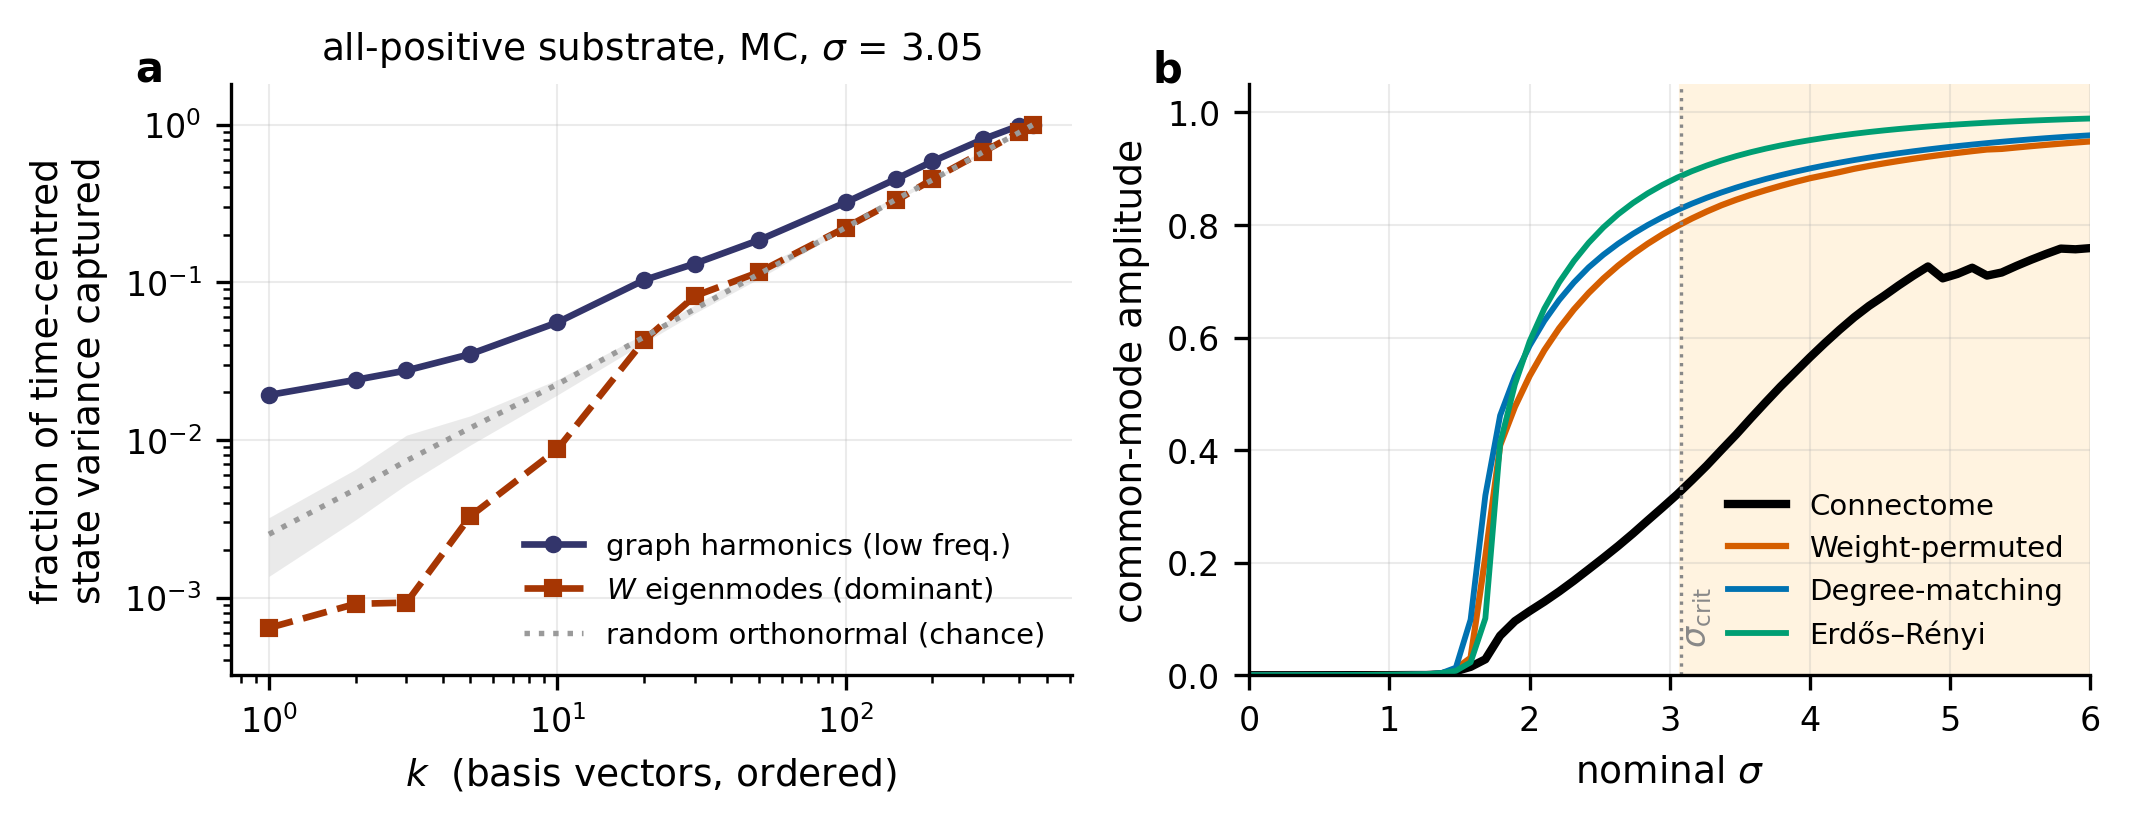
\includegraphics[width=\textwidth]{F4.png}
    \caption[The Perron mode is a common mode]{%
    \textbf{The Perron mode is a common mode: it carries the time-average, and the
    fluctuations the readout uses are orthogonal to it.} Human $N = 448$ % TIER0 2.1
    self-built consensus, all-positive empirical weights, memory-capacity task,
    ten seeds, medians over seeds. \textbf{(a)} Fraction of the \emph{time-centred}
    state variance held by the leading $k$ vectors of three orthonormal bases, on
    the connectome alone at the supercritical operating point
    $\sigma = 3.05$; % COV 3.4
    both axes logarithmic, and not a statement about the null ladder. The dominant
    $W$ eigenmodes fall below the random baseline and reach it only around
    $k = 20$, % A2 F4
    while the graph harmonics on the same states sit well above it. The grey band
    is the across-seed range of the chance curve, which is the quantity the
    per-seed comparison is made against; a single random direction is far more
    variable. Pooled across the capture's three tasks the leading mode holds
    0.0001 % TIER0 3.12
    against a 0.0023 % TIER0 3.12
    baseline, the value of record. \textbf{(b)} Common-mode amplitude against
    nominal $\sigma$ for the four substrates, absolute-valued before medianing
    (Section~\ref{sec:act2-captures}). The connectome is the \textbf{least}
    dominated at every $\sigma$ above roughly 1.5,
    0.759 % TIER0 3.7
    at $\sigma = 6$ against 0.949 to 0.989, % TIER0 3.7
    despite carrying much the largest Perron root
    (Figure~\ref{fig:F2}). The nulls rise first because they become supercritical
    first; the dotted rule is the connectome's own critical scale and the shaded
    region lies above it.}
    \label{fig:F4}
\end{figure}

% P3: A2.2 and the inversion. Refers back to chapter 4 without re-quoting.
So the leading modes are absent from the fluctuations. Panel~(b) of the same
figure asks where they went, by measuring the common-mode amplitude across the
whole sweep in $\sigma$ for all four substrates. Every substrate's rises as it is
driven harder, which is what a network being pushed into the flat regions of its
nonlinearity does, and the nulls' rise first, since they reach their own critical
scales well before the connectome reaches its; those scales are
Chapter~\ref{chapter:act-I}'s and are not re-derived here. What matters is where
the four curves end up. At $\sigma = 6$ % TIER0 3.7
the connectome sits at 0.759 % TIER0 3.7
against the nulls' 0.949 to 0.989, % TIER0 3.7
and near criticality at $\sigma = 2$ % TIER0 3.7
the separation is wider still, 0.114 % TIER0 3.7
against 0.53 to 0.59. % TIER0 3.7
The connectome is the least common-mode dominated substrate on the ladder, and it
is the substrate carrying by far the largest Perron root. That inversion is the
finding of this section. It is not a paradox but a consequence of what
Chapter~\ref{chapter:act-I} measured: what separates the connectome is a gap
between its leading eigenvalue and its bulk, not a leading eigenvalue that is small
or a bulk that is unusual, and a gap of that kind lets the leading mode be driven
hard without the bulk following it. The nulls, whose bulk sits close behind their
Perron root, synchronise as a whole. Their units end up pinned near the extremes of
the nonlinearity together, which is what an amplitude approaching one means, and
almost nothing is left that varies.

% P4: what this establishes and what it does not; poses section 4.
Two things follow, and it is worth separating them from a third that does not. The
decomposition is clean: the leading mode carries the time-average and the bulk
carries what a readout could use, which is what licenses the rest of this chapter
to work in the fluctuation subspace and to treat the rank-one term as accounted
for. And the substrates differ in how much of their activity that rank-one term
consumes, in the direction opposite to the one the spectrum naively suggests. What
does \emph{not} follow is anything about capacity. Being least dominated by the
common mode is not the same as having the most directions a readout can act on, and
the step between them is the one this chapter has yet to measure; nothing above
touches how the fluctuation spectrum is arranged, only how much of the activity is
left in it. That arrangement is what the readout is finally sensitive to, through
the regularisation floor Equation~\ref{eq:deff} counts against, and it is where
Section~\ref{sec:act2-floor} goes next. Everything in this section, and everywhere
else in this chapter, is measured on non-negative weights; no sign manipulation
appears until Chapter~\ref{chapter:act-III}.





\section{The Gram spectrum against the ridge floor}
\label{sec:act2-floor}
\bigskip
% Outline item 4 (act2_manifold.md section 4). Carries A2.6 and A2.7.
% Figure F18 (a, b, c). Chain step 3 in CROSS_ACT_SPINE.md: the measured link
% from weak common-mode domination to usable dimensionality. Sources: sheet 09.
% FORBIDDEN here (sheet 09): "minimum" without "interior", in prose or caption;
% "1.8 to 3.9" as the span of the null minima; "raising alpha costs Erdos-Renyi
% little"; a low sensitivity read as good or bad on its own; "the gap puts the
% Gram spectrum clear of the floor" as though derived here; "the anisotropy
% hypothesis is confirmed", or the decay exponent used as support; "tracks",
% "predicts", or any regression language for the migration; "3.58 is 3.6";
% "four orders"; the published fractions quoted without the zero-strip; any
% sentence implying the four per-bin medians sum to 100; "compact bulk".

% P1: the question, the guard, and A2.6 stated as positions.
Section~\ref{sec:act2-perron} established that the connectome keeps more of its
activity in the fluctuation term than any of its nulls do. It said nothing about
how that activity is arranged, and arrangement is what the readout is sensitive
to: Equation~\ref{eq:deff} counts directions by how far their Gram eigenvalues
stand above the regularisation, so what matters is where each substrate's spectrum
sits relative to that floor. This is a measurement rather than a derivation.
Nothing here obtains the position of the Gram spectrum from the spectrum of $W$,
and the link back to the spectral gap runs through the common-mode account of the
previous section rather than around it. Measured supercritically, the positions
are strikingly different. The connectome holds
89.0\% % TIER0 3.6(e)
of its directions more than a decade clear of the floor, against Erdős–Rényi's
11.4\%; % TIER0 3.6(e)
read from the other end, 73.2\% % TIER0 3.6(c)
of Erdős–Rényi's spectrum lies at or more than a decade \emph{below} the floor
before the regularisation is raised at all, against the connectome's
5.1\%. % TIER0 3.6(c)
That is what $d_{\mathrm{eff}}$
412.9 % TIER0 3.6
against 74.8 % TIER0 3.6
counts, and the two statements are the same fact viewed from either side of the
floor.\footnote{All four statistics are computed on the design-Gram spectrum with
exact zeros removed first, as the implementation does it; the convention is
load-bearing rather than cosmetic, since on the full 448-direction denominator the
published fraction below the floor reproduces for no substrate (the connectome's
6.6\% % TIER0 3.6
reads 7.03\% % TIER0 3.6(a)
and Erdős–Rényi's 79.4\% % TIER0 3.6
reads 83.59\%), % TIER0 3.6(a)
and the error grows down the ladder because the count of numerically rank-deficient
directions does. The other three statistics are untouched: a zero contributes
exactly nothing to $d_{\mathrm{eff}}$ and to the sensitivity below, and is never
within a decade of the floor. Figure~\ref{fig:F18}(a) shows the zeros as a bin of
their own rather than folding them into the fraction below the floor, which makes
the exclusion visible rather than merely stated.}
These are per-bin medians over the fifty supercritical cells of each substrate, so
the bins partition each individual cell exactly while four medians taken separately
are not constrained to sum to one hundred, and the connectome's come to
102.1\%. % TIER0 3.6(e)
Panel~(a) of Figure~\ref{fig:F18} therefore groups its bars rather than stacking
them, since a stacked bar would assert a partition the medians do not form.

% Figure F18.
\begin{figure}[ht]
    \centering
    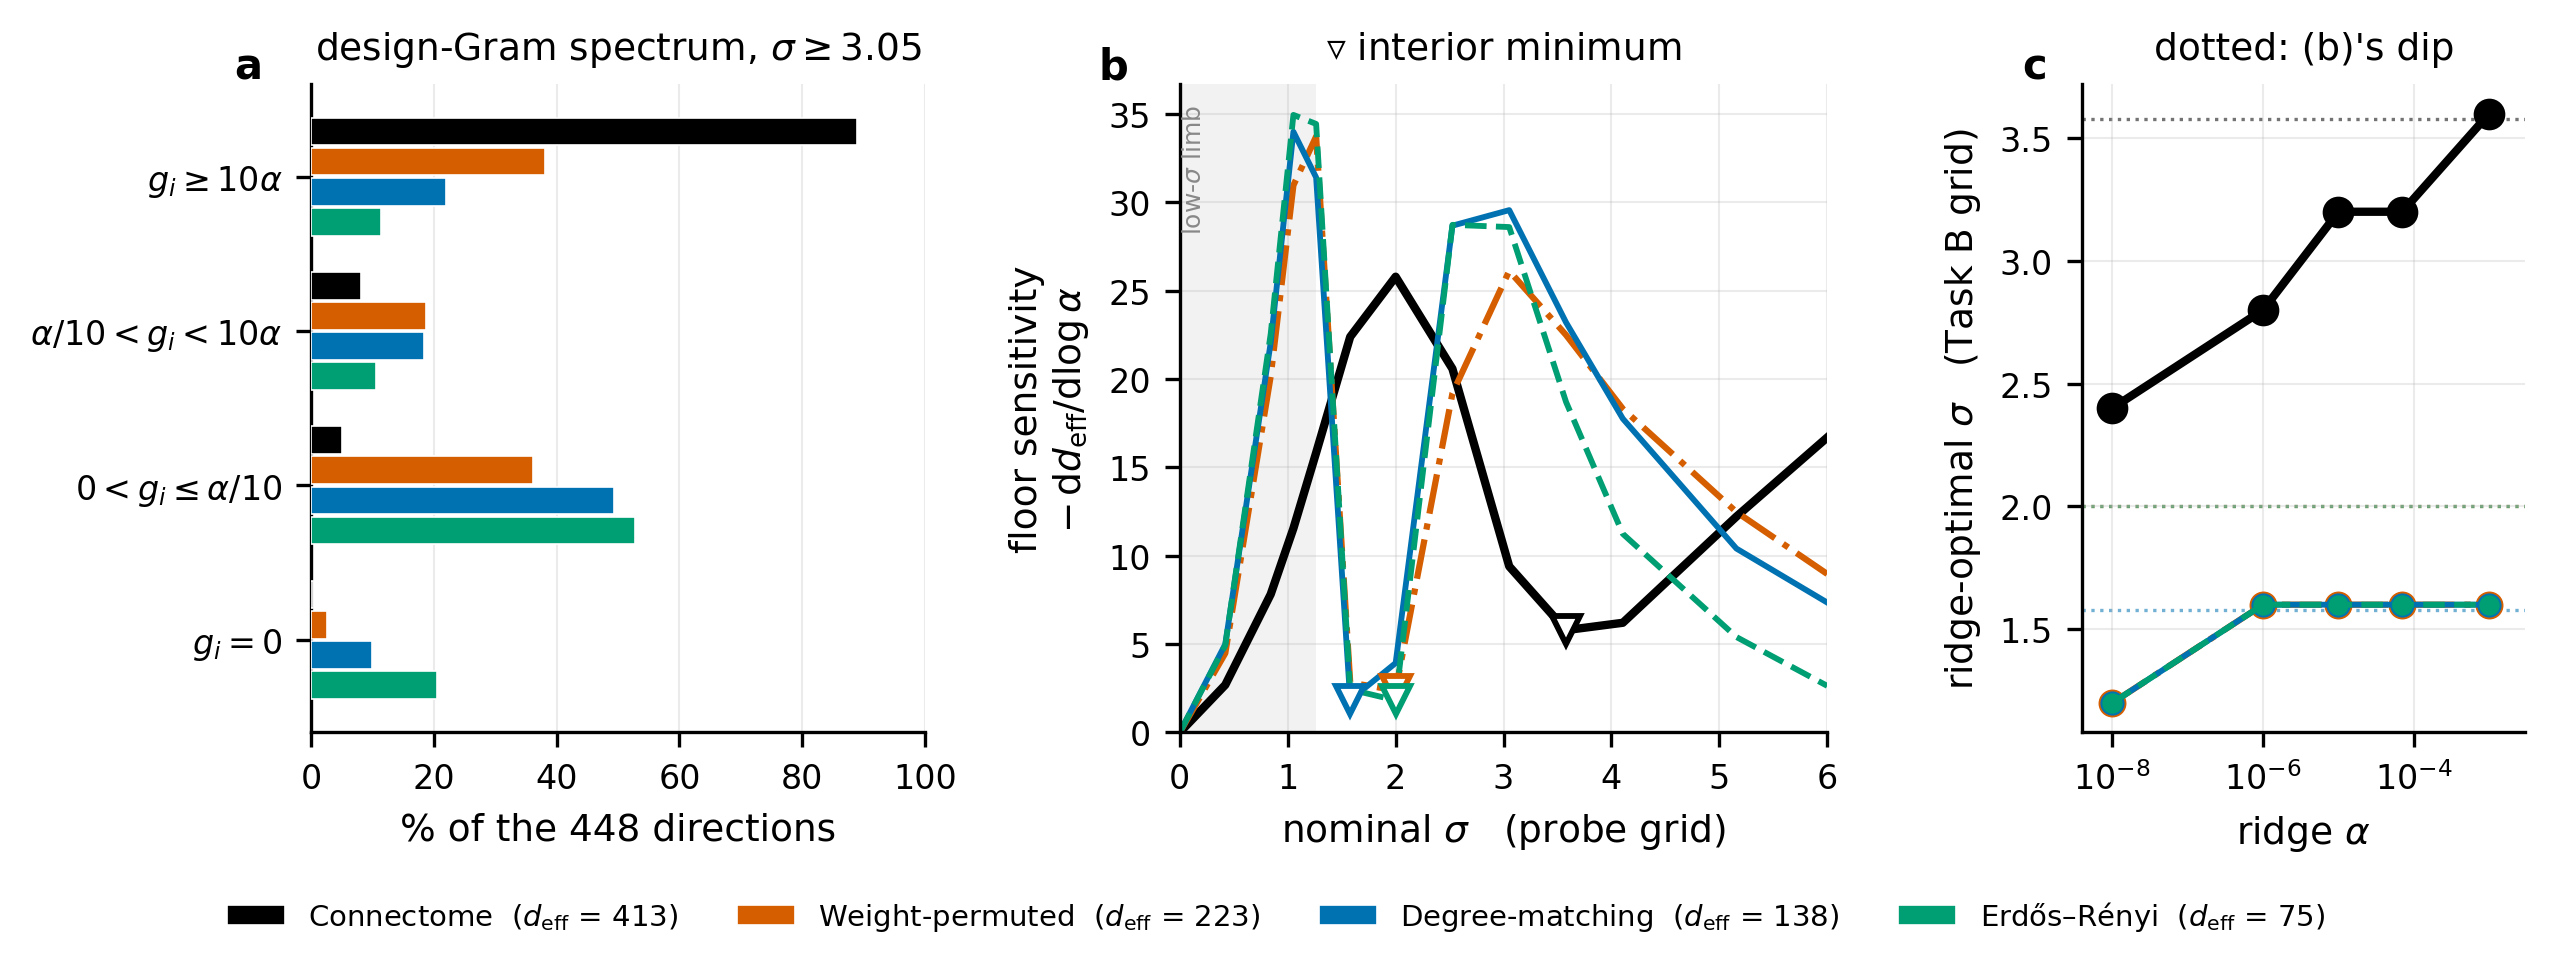
\includegraphics[width=\textwidth]{F18.png}
    \caption[Where the Gram spectrum sits relative to the readout floor]{%
    \textbf{Where the Gram spectrum sits relative to the readout floor is what
    sets usable dimensionality.} Memory-capacity task, all-positive weights,
    $N = 448$, % TIER0 2.1
    ten seeds. \textbf{(a)} Design-Gram eigenvalues by position relative to the
    floor, supercritically, as a percentage of all 448 directions; medians over
    the fifty cells per substrate, with $d_{\mathrm{eff}}$ carried in the legend
    because it is a property of the whole spectrum rather than of any one bin.
    Exact zeros form their own bin and are excluded from the fraction below the
    floor. Bars are grouped, not stacked: the bins partition each individual cell
    exactly, but four medians taken separately need not sum to one hundred.
    \textbf{(b)} Sensitivity of $d_{\mathrm{eff}}$ to the floor against spectral
    radius, whole curve drawn. It vanishes at both ends, so the minima that matter
    are the \emph{interior} dips, marked per substrate; the shaded low-radius limb
    is where the reservoir is too weakly driven to have much spectrum above the
    floor at all, and is excluded from the search. \textbf{(c)} The measured
    ridge-optimal radius against regularisation strength, which migrates toward
    each substrate's own interior dip. The three nulls coincide exactly at every
    value, so their markers nest rather than being offset. Panels~(a) and~(b) use
    the probe radius grid and~(c) the coarser sweep grid, so
    3.58 % TIER0 3.6(b)
    and 3.6 % TIER0 3.6
    are two grids' nearest points to one place rather than the same number. The
    correspondence in~(c) is consistent-with; nothing is fitted.}
    \label{fig:F18}
\end{figure}

% P2: the rate, with the both-ends warning taken off the algebra first.
How much a substrate stands to lose if the regularisation is raised is a different
question from where its spectrum sits, and the two are easy to conflate.
Differentiating Equation~\ref{eq:deff} gives the rate directly:
\begin{equation}
    -\frac{\mathrm{d}\,d_{\mathrm{eff}}}{\mathrm{d}\log\alpha}
    \;=\; \sum_{i=1}^{N} \frac{g_i\,\alpha}{(g_i + \alpha)^{2}},
    \label{eq:floor-sensitivity}
\end{equation}
in units of directions lost per e-fold of $\alpha$. Each term peaks, at one
quarter, when a direction sits exactly \emph{at} the floor, and falls away as it
moves in either direction. So the sum is small for a substrate whose spectrum
stands well clear of the floor and equally small for one whose spectrum has already
fallen far below it, and a low value never interprets itself: only the positions
above tell the two cases apart. Erdős–Rényi is the second case, and reading its
low absolute sensitivity as robustness would invert the truth. Per unit of
surviving dimensionality it is the \emph{most} floor-sensitive substrate on the
ladder, losing 29.1\% % TIER0 3.6(c)
of its effective rank per decade of $\alpha$ against the connectome's
5.6\%. % TIER0 3.6(c)
The absolute losses are nearly the same at the two ends of the ladder,
21.8 % TIER0 3.6(c)
directions against 23.3; % TIER0 3.6(c)
the connectome simply has some four hundred directions to lose them from and
Erdős–Rényi has around seventy-five.

% P3: A2.7 first half, the interior minima.
Neither the positions nor the rate is a fixed property of a substrate, because both
depend on where the substrate is being operated. Panel~(b) draws
Equation~\ref{eq:floor-sensitivity} across the whole sweep, and the curve is
two-humped: it falls to zero at zero radius, where a reservoir barely driven at all
has almost no spectrum above the floor to lose, rises as directions are pushed up
through the floor, and falls again once they are clear of it. The minima that
matter are therefore the \emph{interior} dips between the two humps, and they sit
at different radii for different substrates: the connectome's near
3.58, % TIER0 3.6(b)
every null's between 1.58 and 2.00. % TIER0 3.6(b)
The separation is not an artefact of taking medians, holding in
8 of 10 % TIER0 3.6(b)
seeds for the connectome and 10 of 10 % TIER0 3.6(b)
for each null. The qualifier is not droppable: the connectome's lowest sensitivity
anywhere over non-zero radius is not its interior dip at all but a value of
2.687 % TIER0 3.6(b)
out at radius 0.4211, % TIER0 3.6(b)
below the dip's 5.785, % TIER0 3.6(b)
and read as a global minimum this half of the result does not reproduce. That is
the same trap as the rate: a low sensitivity out on the left-hand limb means a
reservoir with nothing to lose.

% P4: A2.7 second half, the migration, with the retraction folded in.
This radius-dependence closes a loose end. Raising the regularisation penalises
operating points where many directions sit at the floor, so each substrate's best
operating point should move toward its own interior dip, and the measured optima do
exactly that. Across a regularisation grid spanning five orders of magnitude in
four steps, % TIER0 3.6(d)
the connectome's ridge-optimal radius moves from
2.4 to 3.6 % TIER0 3.6
while every null moves once, from 1.2 to 1.6, % TIER0 3.6
each toward its own dip. Two caveats travel with that and are not detachable from
it. The two halves sit on different radius grids, so
3.58 and 3.6 % TIER0 3.6
are two grids' nearest points to one place rather than one number recovered twice.
And the correspondence is consistent-with rather than fitted: what is shown is that
the direction and the endpoint agree for all four substrates, and nothing is
regressed on anything. It is worth recording what this replaces, since an earlier
account explained the same migration differently. The proposal was that the
connectome's optimum moves because its covariance is more anisotropic, so raising
the regularisation strips its directions faster. That is rejected on its own
measurement: of the three substrates tested the connectome has the
\emph{shallowest} covariance decay, so by that measure it is the least anisotropic
rather than the most, and the participation ratio is flat across them at
1.21 to 1.29. % TIER0 3.6
The rejection stands. What survives is the account above, refitted at the other end
of the spectrum, the decay exponent having been fitted over the top decile while
what governs a ridge readout is the bottom.

% P5: handover into section 5.
One consequence of these positions deserves stating before the next section uses
it. The floor sits some ten orders of magnitude % A2 4.5.3
below the leading variance, so a substrate can have hundreds of directions
standing clear of it that carry almost none of the variance between them. Whether
those directions are counted at all depends entirely on how a dimensionality
measure weights them, and the measure the field reaches for first weights by
variance.




\section{Which counting scheme sees it}
\label{sec:act2-counting}
\bigskip
% Outline item 5 (act2_manifold.md section 4). Carries A2.4 and A2.5, together
% contribution 6. Figure F6 (a, b, c). Chain step 4 in CROSS_ACT_SPINE.md.
% Sources: fact sheet 10.
% FORBIDDEN here (sheet 10): any sentence carrying one number from the seven-rung
% unit and one from the 350-cell unit; the rung-index correlation quoted as the
% result; "+0.54" for its PR value (sign corrected to negative); "PR is wrong";
% "d_eff is a better measure in general"; PR's failure as a separate finding; any
% mechanism for why the low-variance directions carry memory; 431 and 413 used
% interchangeably; "peak d_eff shows the connectome uses more directions";
% "the manifold lives in low-frequency graph harmonics"; "compact bulk".

% P1: the range first, because the range is the mechanism.
Put the same seven substrates through the same task and measure the dimensionality
of the states they produce, and the answer depends on which measure is used to an
extent that ought to be alarming. The ridge effective rank moves
5.5-fold % TIER0 3.12
across them, from 75 to 413 % TIER0 3.12
of the 448 directions available. The participation ratio, the variance-weighted
count the field reaches for first, moves
16\%, % TIER0 3.12
from 1.19 to 1.38. % TIER0 3.12
These are not different experiments. They are two functions of the same stored
spectra, computed on the same cells, and one of them says these substrates differ
enormously while the other says they are barely distinguishable. Measured memory
capacity moves roughly three-fold % A2 2.2
over the same substrates, so there is something there to be seen. The question is
what makes one measure blind to it.

% P2: both are weighted counts over one matrix; the mechanism in one cell.
The two measures are more alike than their disagreement suggests, which is what
makes the disagreement informative. Both are exactly sums of one weight per
direction of the same state matrix. For the ridge effective rank that is
Equation~\ref{eq:deff} as written, each direction weighted by
$g_i/(g_i + \alpha)$, how far its Gram eigenvalue clears the regularisation floor.
For the participation ratio it is true but less obvious. Writing
$p_i = \lambda_i / \sum_j \lambda_j$ for direction $i$'s share of the state
covariance,
\begin{equation}
    \mathrm{PR}
    \;=\; \frac{\bigl(\sum_i \lambda_i\bigr)^{2}}{\sum_i \lambda_i^{2}}
    \;=\; \sum_{i=1}^{N} \frac{p_i}{\sum_j p_j^{2}},
    \label{eq:pr}
\end{equation}
so it too is a sum of per-direction weights, each direction counted by its share of
the variance. Both are therefore counts, and each curve's area in
Figure~\ref{fig:F6}(a) is the number it is labelled with. What the panel shows on
one connectome cell is how differently the two weight the same directions: the
ridge weight is above one half for
438 of the 448 % A2 2.4
directions, while the variance weight has collapsed by the fifth, with
two directions carrying 95\% % A2 2.4
of a participation ratio of 1.28. % A2 2.4
The covariance and the Gram are formed on one and the same post-warmup state
matrix, so the difference between them is one of weighting and not of data.

% Figure F6.
\begin{figure}[ht]
    \centering
    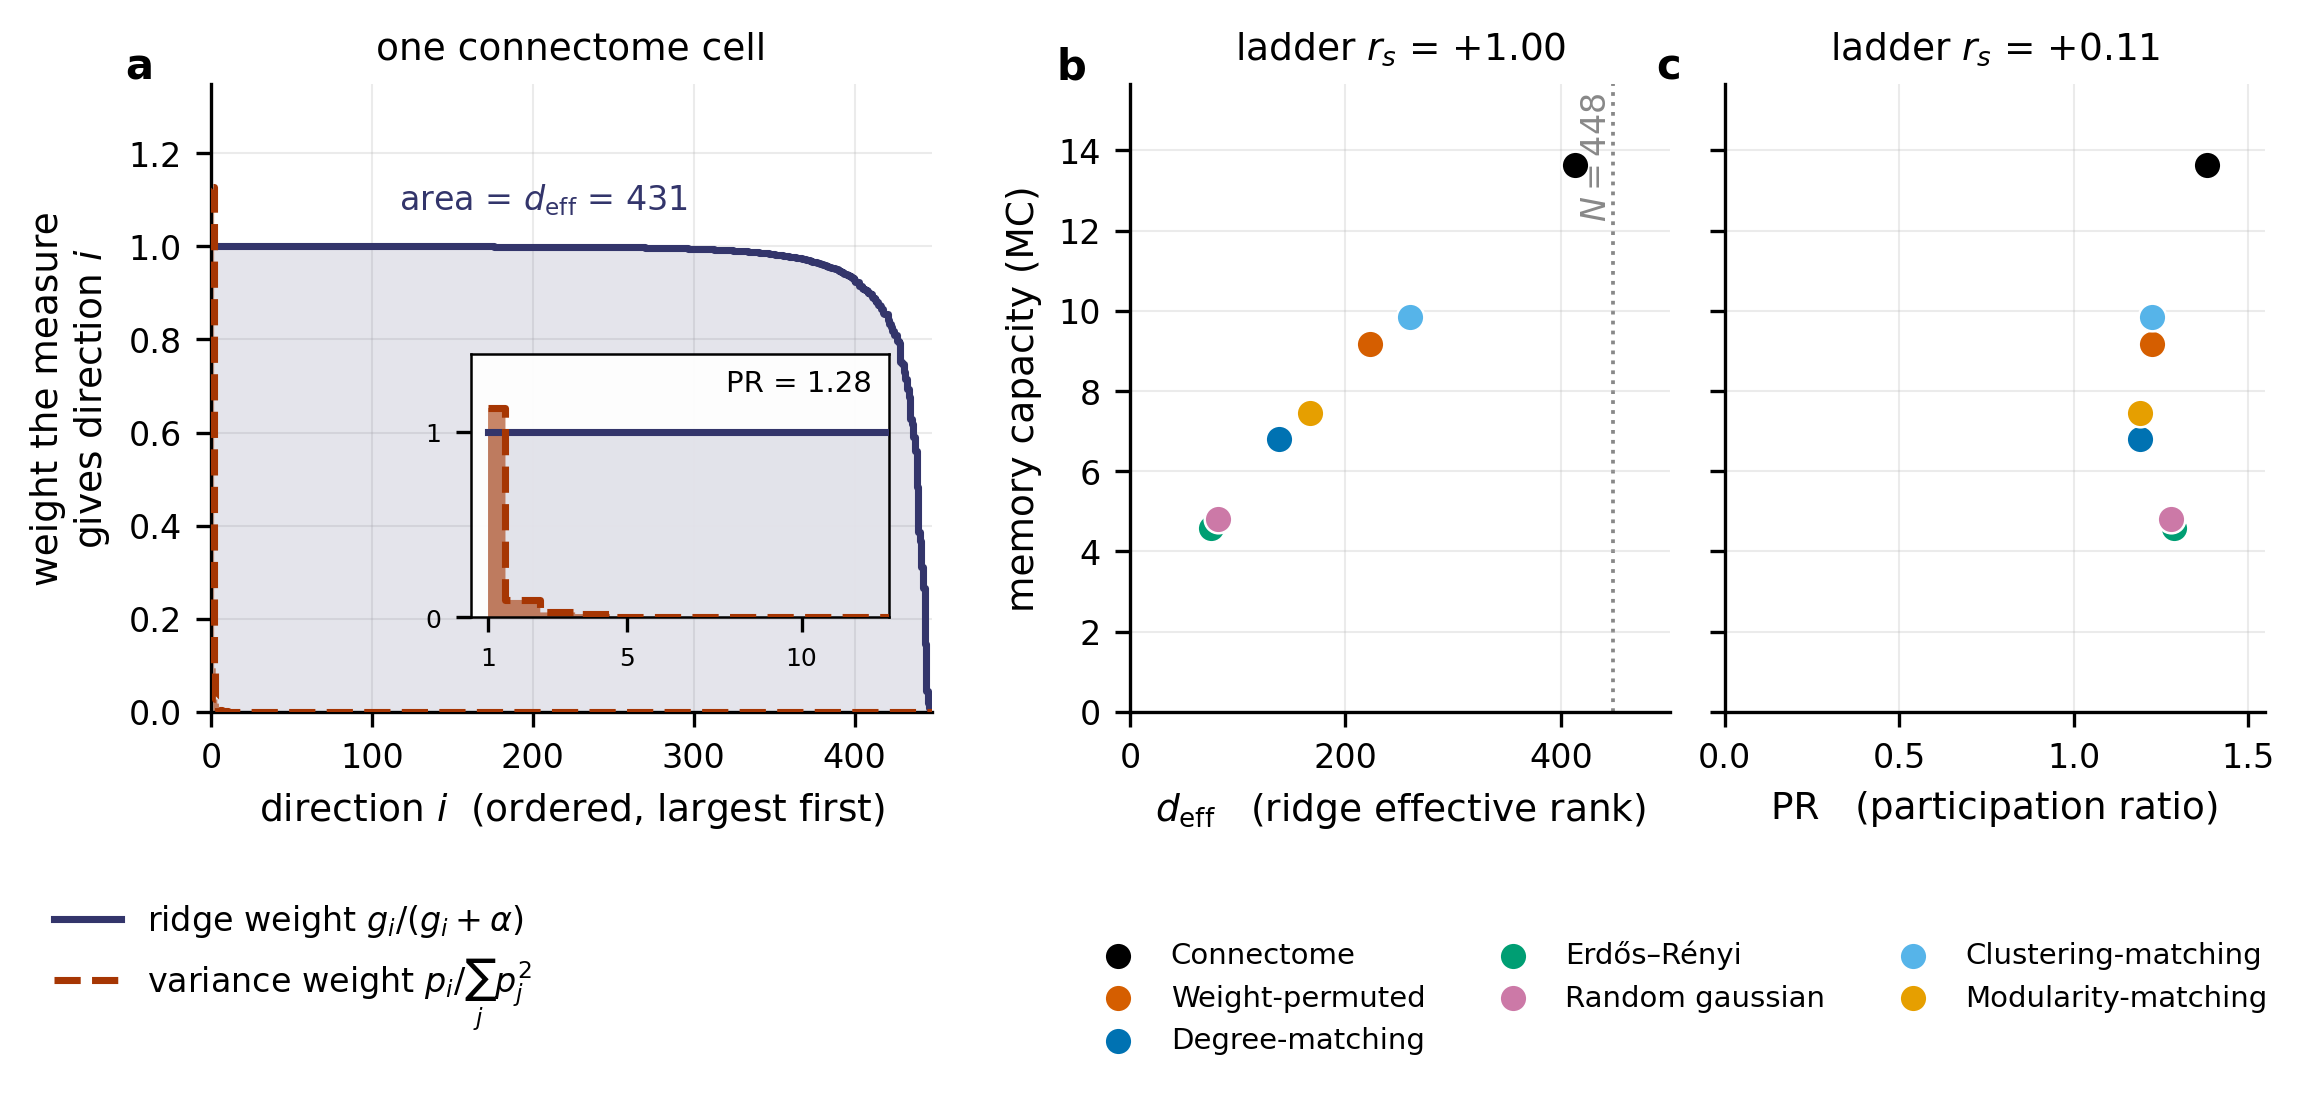
\includegraphics[width=\textwidth]{F6.png}
    \caption[Memory lives in low-variance directions that a variance-weighted
    measure discounts]{%
    \textbf{Memory lives in hundreds of low-variance directions, which a
    variance-weighted measure discounts.} Memory-capacity task, all-positive
    weights, $N = 448$, % TIER0 2.1
    supercritical cells. \textbf{(a)} The per-direction weight each measure
    assigns, on \emph{one} connectome cell, with a zoom over the first twelve
    directions on the same linear scale. Both measures are exact sums of these
    weights, so each shaded area is the number beside it. This cell's effective
    rank is 431; % A2 2.4
    the connectome's median over all fifty supercritical cells, plotted in~(b), is
    413. % TIER0 3.6
    \textbf{(b, c)} The consequence across the seven substrates of the wider null
    ladder, medians over fifty cells each, against \textbf{measured} memory
    capacity. Both axes are zero-based, so the spread of the points is comparable
    between panels: over the same substrates the effective rank moves
    5.5-fold % TIER0 3.12
    while the participation ratio moves 16\%. % TIER0 3.12
    Panel~(b)'s upper limit is the hard ceiling at $N$. Both correlations reported
    in the text are against measured memory capacity, never against ladder
    position, which is a different quantity and is not the claim.}
    \label{fig:F6}
\end{figure}

% P3: PR's failure is a consequence of section 4.
That collapse is not a separate finding. It follows from where the spectrum sits,
which Section~\ref{sec:act2-floor} has just measured. The regularisation floor lies
some ten orders of magnitude below the leading variance, so a direction can stand
far clear of the floor, and be fully available to the readout, while holding a
share of the variance too small to register in a weighted count. Hundreds of the
connectome's directions are in exactly that position. A variance-weighted measure
does not fail here through any defect of its own; it fails because the quantity it
weights by and the quantity that determines availability have come apart, and they
come apart precisely where the previous section found the substrates to differ.

% P4: the test against measured MC, one aggregation unit per sentence.
Whether that matters is a question the data can answer, by asking which measure
tracks what the readout actually achieves. Memory capacity enters here as the
quantity a dimensionality measure is being judged against, not as a performance
claim about any substrate: what is being ordered is the counting schemes, not the
connectome and its nulls. Across the seven substrates, taking one median per
substrate, the ridge effective rank orders them against measured capacity at a rank
correlation of +1.000 % TIER0 3.12
and the participation ratio at +0.107. % TIER0 3.12
Pooled instead over all 350 % TIER0 3.12
individual cells within the supercritical regime, the pair reads
+0.998 % TIER0 3.12
against +0.308. % TIER0 3.12
Those are two separate tests on two aggregation units, and a number from one may
not be set against a number from the other, though the two agree on everything that
matters. Correlating either measure against position in the null ladder is a
different quantity again, weak and negative for both, and is not the claim being
made. One limit belongs with this, since it bounds what the ordering can mean:
every substrate's effective rank peaks within a few per cent of the hard ceiling at
$N$, % TIER0 3.2
so peak dimensionality is unresolvable at this parcellation and the ordering above
lives in the decay region beyond the peak rather than at it.

% P5: observer-relativity owned, then scope.
The natural way to write this result is that the participation ratio is wrong, and
that would be the wrong way. It measures what it claims to measure, which is how
concentrated the variance of the states is, and for a question about the shape of
the activity cloud it is the right instrument. The claim here is narrower and, I
think, more interesting: that quantity is not the one a ridge readout can act on,
so a measure of dimensionality is only meaningful relative to what is reading the
system out. Two measures of the same states can disagree by 5.5-fold against 16\%
without either being in error, and the choice between them is a question about the
observer rather than about the data. The demonstration is empirical and its scope
should be read narrowly: one task, one family of substrates, one readout. That
total capacity is bounded by the number of linearly independent state variables is
established, and this is a case of that bound rather than a rival to
it~\cite{dambre2012information}; and the effective rank counted here is a property
of the states a task drives the network through, not of the recurrent matrix, which
is a distinct quantity that shares the
name~\cite{clark2025connectivity}.




\section{Sign selects the basis}
\label{sec:act2-sign}
\bigskip
% Outline item 6 (act2_manifold.md section 4). Carries A2.3, the one claim in the
% act that is deliberately NOT a contribution. Figure F5 (a, b, c). Short, and
% framed as a statement about the decomposition rather than about sign.
% Sources: fact sheet 11.
% FORBIDDEN here (sheet 11): "the manifold lives in low-frequency graph
% harmonics"; any ladder reading of this capture (two substrates only);
% "sign-gating of the manifold transition is a new result"; "balancing the signs
% improves the representation"; quoting the capture values as evidence of how
% much structure the bases hold; treating this as a result about the sign
% fraction f, which is chapter 6's intervention; "compact bulk"; any graded
% curvature account.

% P1: the question the decomposition leaves open, and why it is settled here.
One question has been left open since Section~\ref{sec:act2-perron}, and it is
worth returning to now that the previous section has supplied what is needed to
answer it properly. With non-negative weights the leading eigenmodes of $W$ were
absorbed into the rank-one term of Equation~\ref{eq:gram-split}, which leaves the
fluctuations to be organised by something other than the dynamical modes
themselves. What organised them, in Figure~\ref{fig:F4}(a), was the low-frequency
harmonics of the graph Laplacian, the smoothest patterns the wiring supports, which
enter the comparison because connectome-defined harmonic modes have been shown to
structure measured cortical
activity~\cite{atasoy2016human}. That result is easy to read as a fact about the
connectome. It is not. It is a fact about non-negativity, and the way to show as
much is to remove the non-negativity and leave everything else where it is.
Balancing the signs of the weights destroys the Perron guarantee, so there is no
dominant common mode for the leading eigenmodes to be absorbed into, and the
prediction is simply that they should come back.

% P2: A2.3, stated as the swap, with the qualifier that stops the overstatement.
They do. Figure~\ref{fig:F5} repeats the basis comparison across three weight
conditions on one substrate and one task: the empirical weights used throughout
this chapter, the same magnitudes with their signs balanced, and gaussian weights.
At $k = 10$ the harmonics hold 0.168 % TIER0 3.12
of the time-centred variance against the $W$ eigenmodes'
0.004 % TIER0 3.12
with non-negative weights; balancing the signs reverses it to
0.019 against 0.081; % TIER0 3.12
and with gaussian weights the eigenmodes hold
0.522 % TIER0 3.12
against 0.012. % TIER0 3.12
The ordering swaps, it swaps in the same direction on the other two tasks the
capture holds, and the topology never changes: the same graph, the same edges, the
same weight magnitudes in the first two conditions, with only the signs
redistributed. What is claimed is the swap. It is worth being explicit that nothing
stronger is available, because the numbers invite it: on the all-positive substrate
neither basis holds much of anything, the whole range across bases and tasks
running 0.04 to 0.17, % TIER0 3.12
so a claim that the fluctuations live in graph harmonics would overstate what has
been measured. Which basis leads is the measurement; how much either one captures
is a separate question, and the answer to that one is "not much".

% Figure F5.
\begin{figure}[ht]
    \centering
    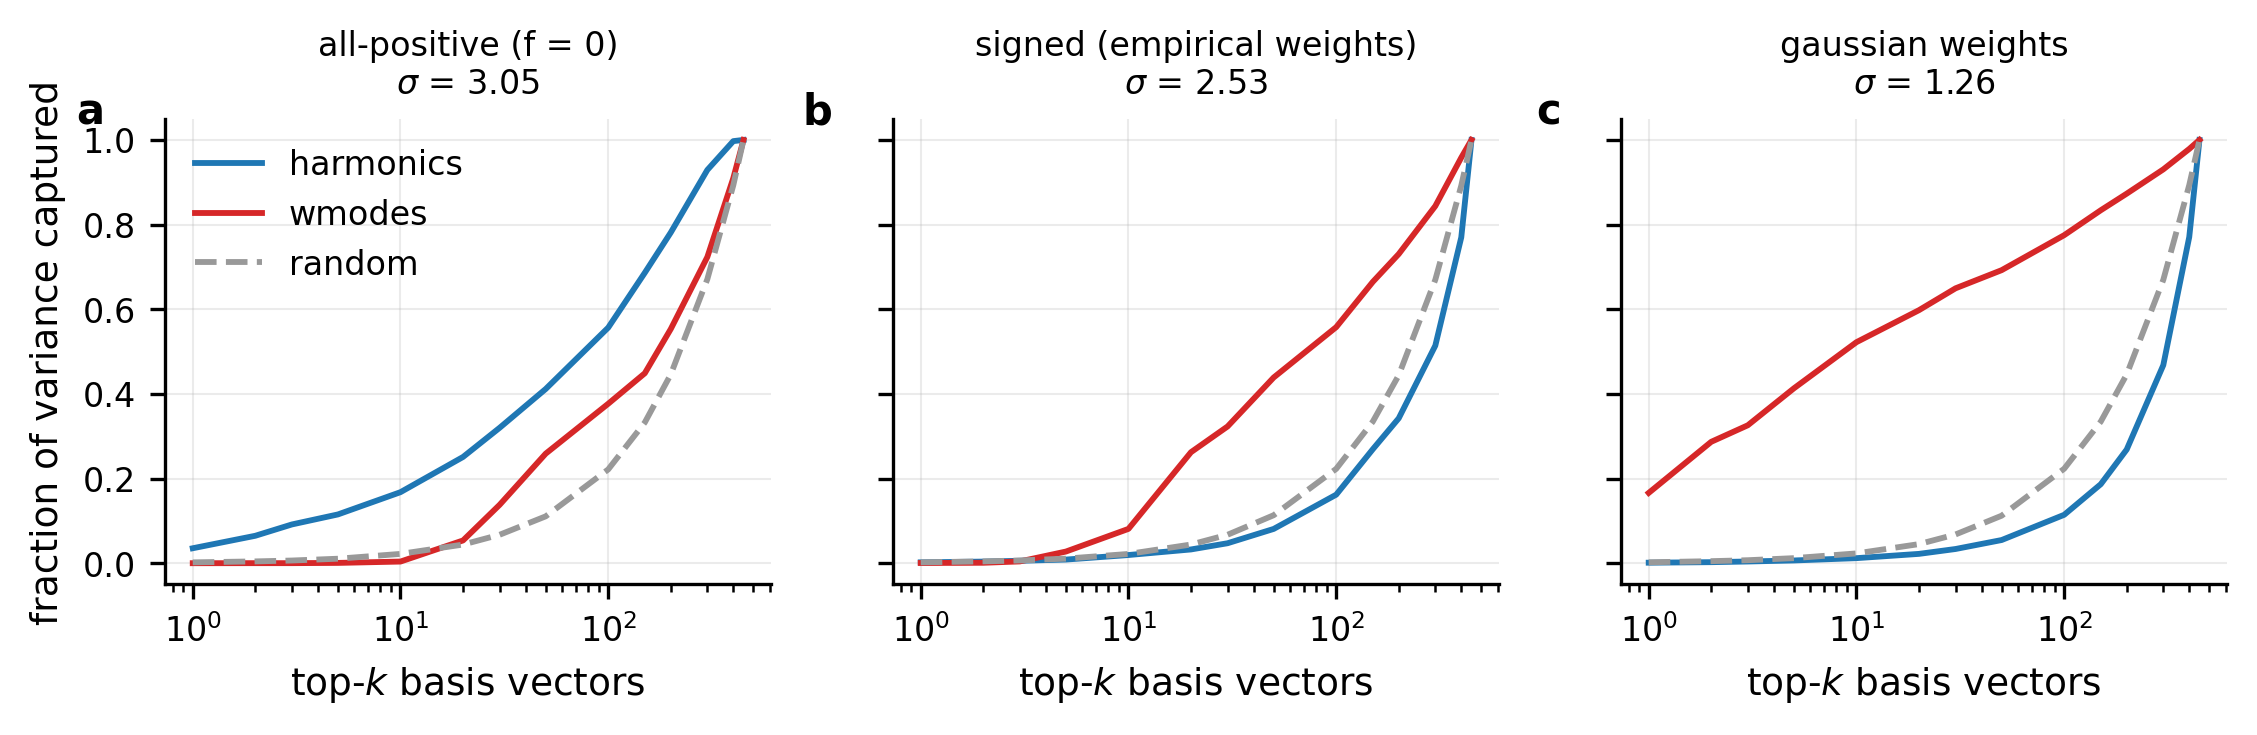
\includegraphics[width=\textwidth]{F5.png}
    \caption[Sign composition selects which structural basis the fluctuations
    occupy]{%
    \textbf{Which structural basis the fluctuations occupy is set by the weight
    signs, not by the topology.} Fraction of time-centred state variance held by
    the leading $k$ vectors of each basis, connectome substrate, Lorenz task,
    $N = 448$, % TIER0 2.1
    medians over ten seeds, each panel at its own condition's supercritical
    operating point. \textbf{(a)} With \textbf{non-negative} weights the graph
    harmonics lead throughout and the dominant $W$ eigenmodes run below chance.
    \textbf{(b)} With the \textbf{same weight magnitudes} and balanced signs the
    ordering has already reversed. \textbf{(c)} With \textbf{gaussian} weights the
    eigenmodes dominate outright. The rule marks $k = 10$, where the values quoted
    in the text are read; the swap is visible across the whole curve, and the
    topology is identical in all three panels. On the all-positive substrate
    neither basis holds much in absolute terms, which is why what is claimed is the
    ordering. Two substrates only: this capture cannot speak to the null ladder.}
    \label{fig:F5}
\end{figure}

% P3: the agreement with section 5, then priority and the forward clause.
The low capture in panel~(a) is not a disappointment but a confirmation, and it is
here that the two halves of this chapter meet without having been made to.
Section~\ref{sec:act2-counting} found that on this substrate, supercritically, the
readout has around 413 % TIER0 3.6
of 448 directions available to it. Fluctuations spread over hundreds of directions
are fluctuations that no ten-vector basis should be able to hold, so the small
captures in panel~(a) are what the other measurement predicts. The relationship
holds at the other end too: where a condition's effective rank is low the capture
is high, reaching 0.886 % TIER0 3.12
on the gaussian weights for one of the tasks this capture covers. Two probes
measuring different things on different bases agree about which substrates and
conditions spread their activity widely, and neither was fitted to the other. Two
final points, both of which place this section rather than extending it. The first
is priority: that weight sign composition gates this transition is largely
pre-empted by Krauss et al.~\cite{krauss2019weight}, and it is reported here as
confirmatory. It earns its place in this chapter because the counting argument of
the previous section needs the basis established first, not because it is new. The
second is scope. The signed and gaussian conditions above are weight families
compared side by side, nothing has been done to the connectome to produce them, and
the question of what happens when negative weights are introduced as an
intervention on the real substrate belongs to Chapter~\ref{chapter:act-III}, where
it is used to remove the common mode and check whether its consequences go with it.









    \chapter{Geometry Governs Computational Capacity}
\label{chapter:act-III}


The previous chapter measured what a driven network's activity looks like, and
left two things unfinished. The first is that how many directions a readout can
use turned out to be a property of a substrate \emph{at an operating point}
rather than of the substrate alone (Section~\ref{sec:act2-floor}), so a
network's capability is a curve and has to be read across its range. The second
is that the common mode was offered as what those differences are made of, and
never shown to be: every substrate compared there carries non-negative weights,
so every one of them carries a common mode, and no comparison among them can
isolate it. This
chapter reads the curve, and then takes the mode away.

Two demands are put to these networks. Memory asks a network to reconstruct an
input it has already been given, which requires that traces of the past remain
separable in the present state. Prediction asks it to sustain a signal with
nothing arriving to correct it, the network driving itself from its own output.
The memory-capacity task puts the first demand directly, scoring the fraction of
a noise input a readout recovers at each of a range of delays and summing across
them, so that capacity is read in units of delays retained. Closed-loop
prediction of the chaotic Lorenz system puts the second, and
Chapter~\ref{chapter:methods} gives the details of both protocols.

Memory separates these substrates, but not where it was looked for. At its own
best operating point each one is using very nearly every direction available to
it, so peak capacity cannot be resolved at this size, and what can be compared
there amounts to parity. What separates them is what survives being driven away
from that point, and there the ordering reverses: the substrate whose peak sits
lowest of the four retains by far the most. The advantage is a width rather than
a height.

Removing the common mode says what that width is made of. Making a fraction of
the weights negative dissolves the guarantee that produces the mode, leaving the
topology and the weight magnitudes as they were, and the memory ladder closes
with it. It does not close in the direction the word removal suggests. No
substrate is harmed by the intervention; supercritical memory rises for all four,
and the advantage disappears because the nulls catch up from far below. What the
connectome's spectral gap supplies is therefore a rescue from a handicap that
non-negativity imposes on everyone, and not a capacity of its own.

The same intervention read on prediction does the opposite. Negative weights
bring a second dynamical branch within reach, and a network falls onto one branch
or the other rather than moving between them: a single bit recording which one
accounts for almost everything the full trajectory geometry accounts for. An
advantage opens where none existed, and across a band of sign fractions the
connectome is the only substrate still predicting usefully. One structural
property is therefore read by the two demands with opposite sign: the sign
composition that buys one costs the other, on every substrate tested.

One thing leaves this chapter unresolved, and it sits inside the account rather
than beside it. On the non-negative weights the instrument actually produces,
prediction is lost across the operating range with no geometric event of any
kind, so the mechanism this chapter assembles is built on a quantity that
registers nothing in exactly the regime the substrate occupies. What governs
that loss is named as an open problem and left that way.



\section{Memory beyond the peak}
\label{sec:act3-memory-sigma}
\bigskip

The primary variable of this chapter is the operating point: how hard the
recurrent dynamics are driven, set by rescaling each connectivity matrix to a
nominal spectral radius $\sigma$. Section~\ref{sec:act1-handover} sets out the
two axes that rescaling makes available and why neither of them is neutral. What
is worth restating here is the consequence for this chapter's claim in
particular: the matched-bulk axis leaves the Perron root unmatched, and so hands
the connectome more of the very quantity proposed as the cause. Every result
below names the axis it was measured on.

Memory is read here through the ridge effective rank of the driven states,
$d_{\mathrm{eff}}$, which counts how many directions of their un-centred Gram
matrix stand clear of the readout's regularisation floor and are therefore
available to a linear map. Chapter~\ref{chapter:act-II} established it as the
quantity that tracks measured memory capacity across substrates, where the
variance-weighted count does not, and it is used in place of the task score
wherever the argument turns on how many directions exist rather than on what a
particular readout recovers from them. Because a network of $N$ units has $N$ directions to offer,
$d_{\mathrm{eff}}$ is bounded above by $N$.

Matched on the bulk radius, all four substrates rise together, all four come
within a few percent of that bound, and they separate only as the dynamics are
driven further into the supercritical regime (Figure~\ref{fig:F7}). The connectome's peak is the lowest
of the four, at
$432.4$ of a possible $448$. % TIER0 1.2
At the top of the range every substrate and every seed covers, it holds
$47\%$ % TIER0 1.2
of that peak against the nulls'
$28$, $22$ and $11\%$. % TIER0 1.2
The ordering at the peak and the ordering deep in the supercritical regime are
opposite, and the crossing between them, rather than either ordering alone, is
the result. That crossing is not an artefact of the axis that produces it, since
the same retention ordering holds on the nominal axis, % TIER0 1.2
but neither is it a global advantage: on that axis it runs the other way below
criticality, and it is absent near the peak on both. Where the bulk is held
fixed, the defensible summary is parity below criticality and advantage above it.

\begin{figure}[htbp]
    \centering
    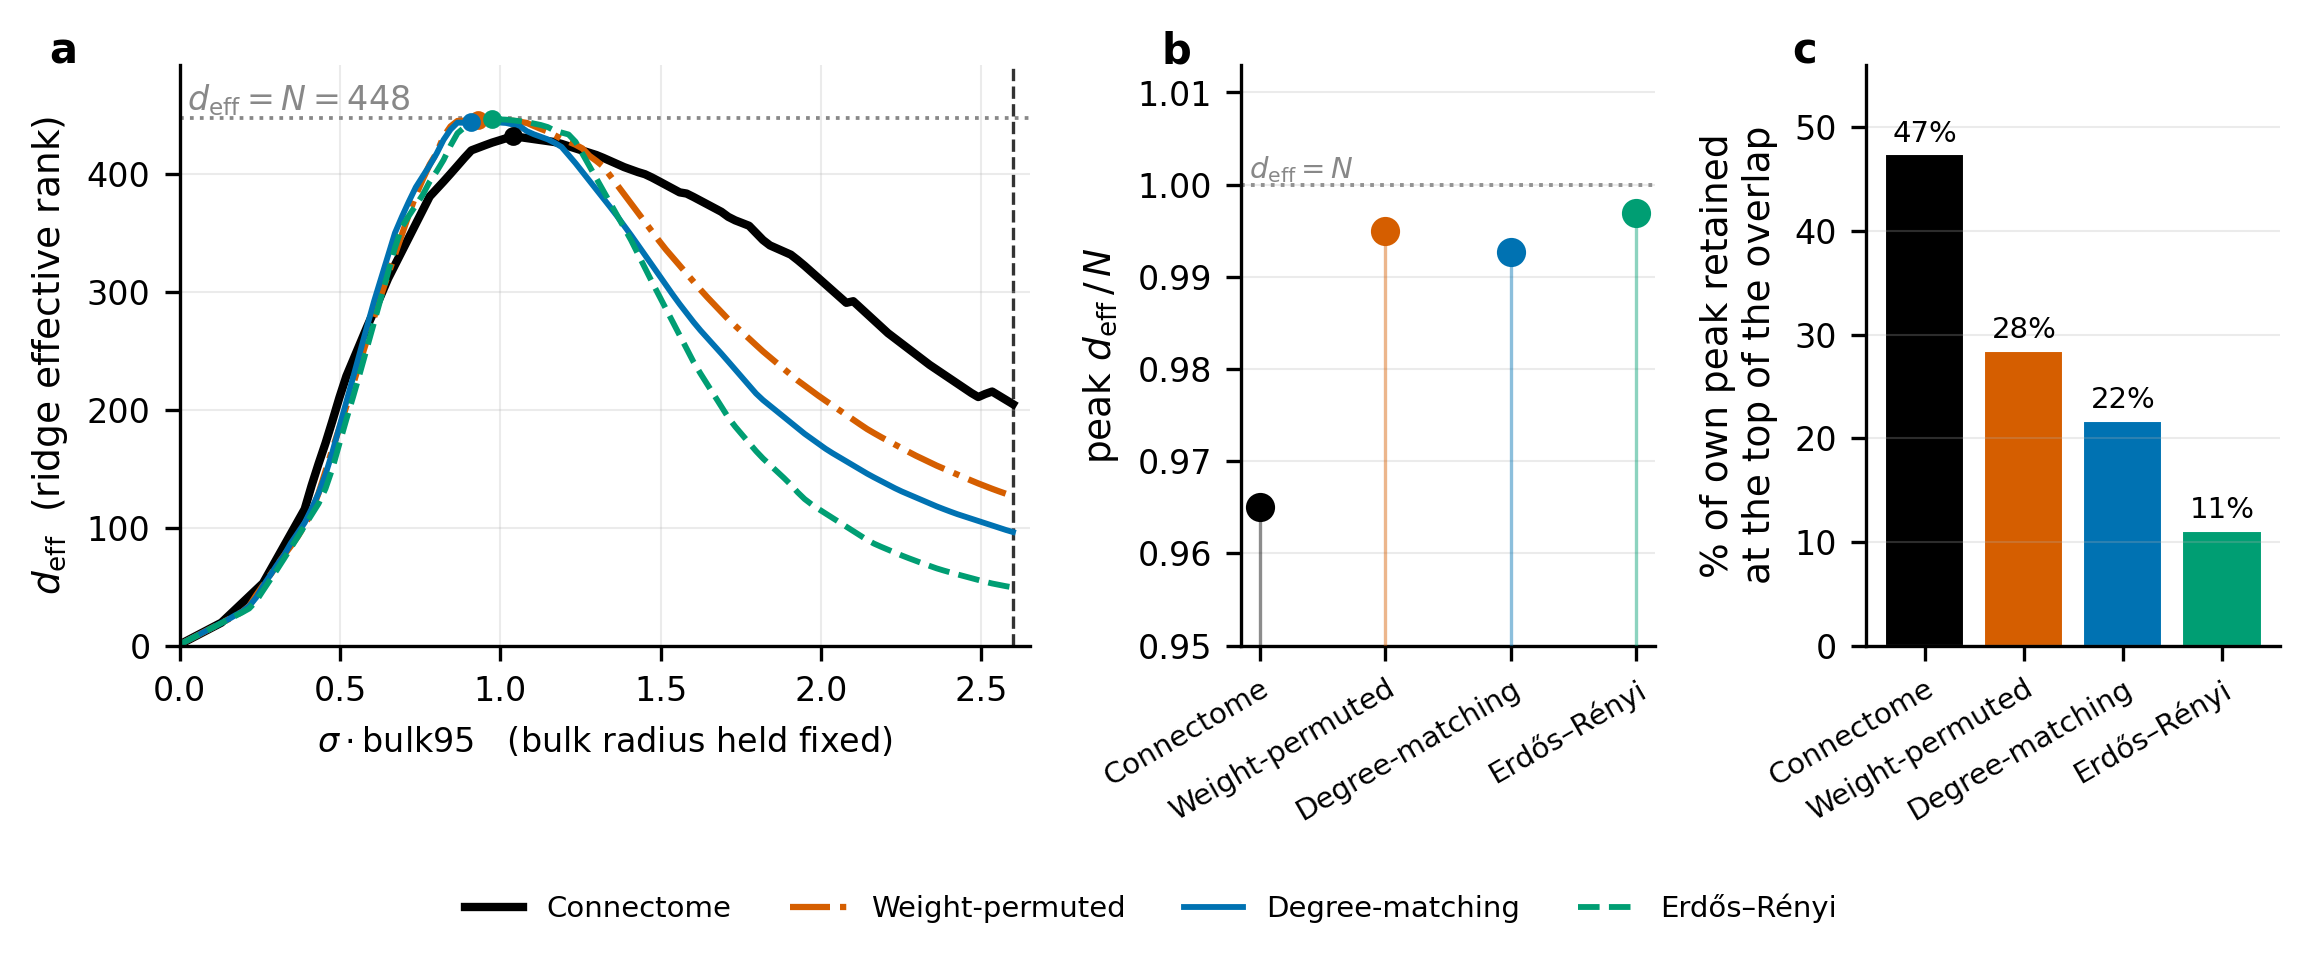
\includegraphics[width=\textwidth]{F7.png}
    \caption[Matched on the bulk radius, the connectome peaks lowest and retains
    most]{\textbf{Matched on the bulk radius, the connectome peaks lowest and
    retains most: the memory result is a crossing, not a capacity difference.}
    Memory-capacity task, $N = 448$, non-negative weights, ten seeds, ridge
    $\alpha = 10^{-6}$. \textbf{(a)} Ridge effective rank against
    $\sigma \cdot \mathrm{bulk95}$, the axis that holds the bulk radius fixed.
    $\mathrm{bulk95}$ is a per-seed quantity for the three resampling nulls, so each
    seed is reindexed onto a common grid before the median is taken; the dashed rule
    at $2.599$ marks the top of the range every substrate and every seed covers. All
    four rise together to the $d_{\mathrm{eff}} = N = 448$ ceiling and separate only
    on the way down. \textbf{(b)} At the peak they are not separable: each lands
    within $3.5\%$ of the ceiling, the connectome at $0.965$ against the nulls'
    $0.993$ to $0.997$. \textbf{(c)} Retention is separable and is the result: at the
    rule in (a) the connectome holds $47\%$ of its own peak against $28$, $22$ and
    $11\%$. A ceiling can clip curves but cannot manufacture a crossing.}
    \label{fig:F7}
\end{figure}

That the peak cannot carry a claim is a limit of the measurement rather than a
retreat from it. Each substrate at its own optimum is using very nearly every
direction available to it, within a few percent of the ceiling, % TIER0 1.2
and the larger network reported below does not escape that ceiling either.
What is resolvable is what happens as the networks are driven past that point,
and a difference there is robust to finite size in a way a difference between the
optima is not.

The peaks can still be compared, and the comparison runs against the chapter's
direction. Paired within seed, each substrate at its own optimum and each pair
sharing input weights and input series, the connectome's peak memory capacity
sits
$2$ to $6\%$ % TIER0 3.4
below the nulls'. Against degree-matching the difference is not consistently
signed, and against the other two nulls it is small and consistent.
Appendix~\ref{app:peak-parity} gives the comparison in full, across five ridge
strengths, and shows there that the ordering reported by Aceituno et
al.~\cite{aceituno2020tailoring} reproduces exactly on these substrates at the
smallest ridge. The defensible statement is parity at the peak rather than a
deficit: the crossing above is not a weak network falling from a lower start.

Whether the result is an artefact of the parcellation is settled by repeating the
memory sweep at
$N = 1000$, % TIER0 2.4
read on measured memory capacity rather than on ridge effective rank
(Figure~\ref{fig:F9}). The supercritical margin holds, and what counts as
supercritical decides how it should be read. Applying the connectome's own
critical scale to every variant, the connectome-to-Erdős--Rényi margin is
$4.40$ at the smaller size and $4.42$ at the larger; % TIER0 2.4
taking each variant above its own critical scale instead gives
$3.56$ and $3.85$. % TIER0 2.4
The first filter leads because it evaluates every substrate over an identical
range of operating points, and it is also the one that flatters the
connectome, since it samples each null further above its own critical point than
the null's own scale would. What survives both is that the margin is not an
artefact of the smaller network; what does not is calling it scale-invariant
without naming the filter. Appendix~\ref{app:scale} gives the protocol, the
control separating the two changes in play, and the one pre-registered test this
run was designed to settle and did not.

\begin{figure}[ht]
    \centering
    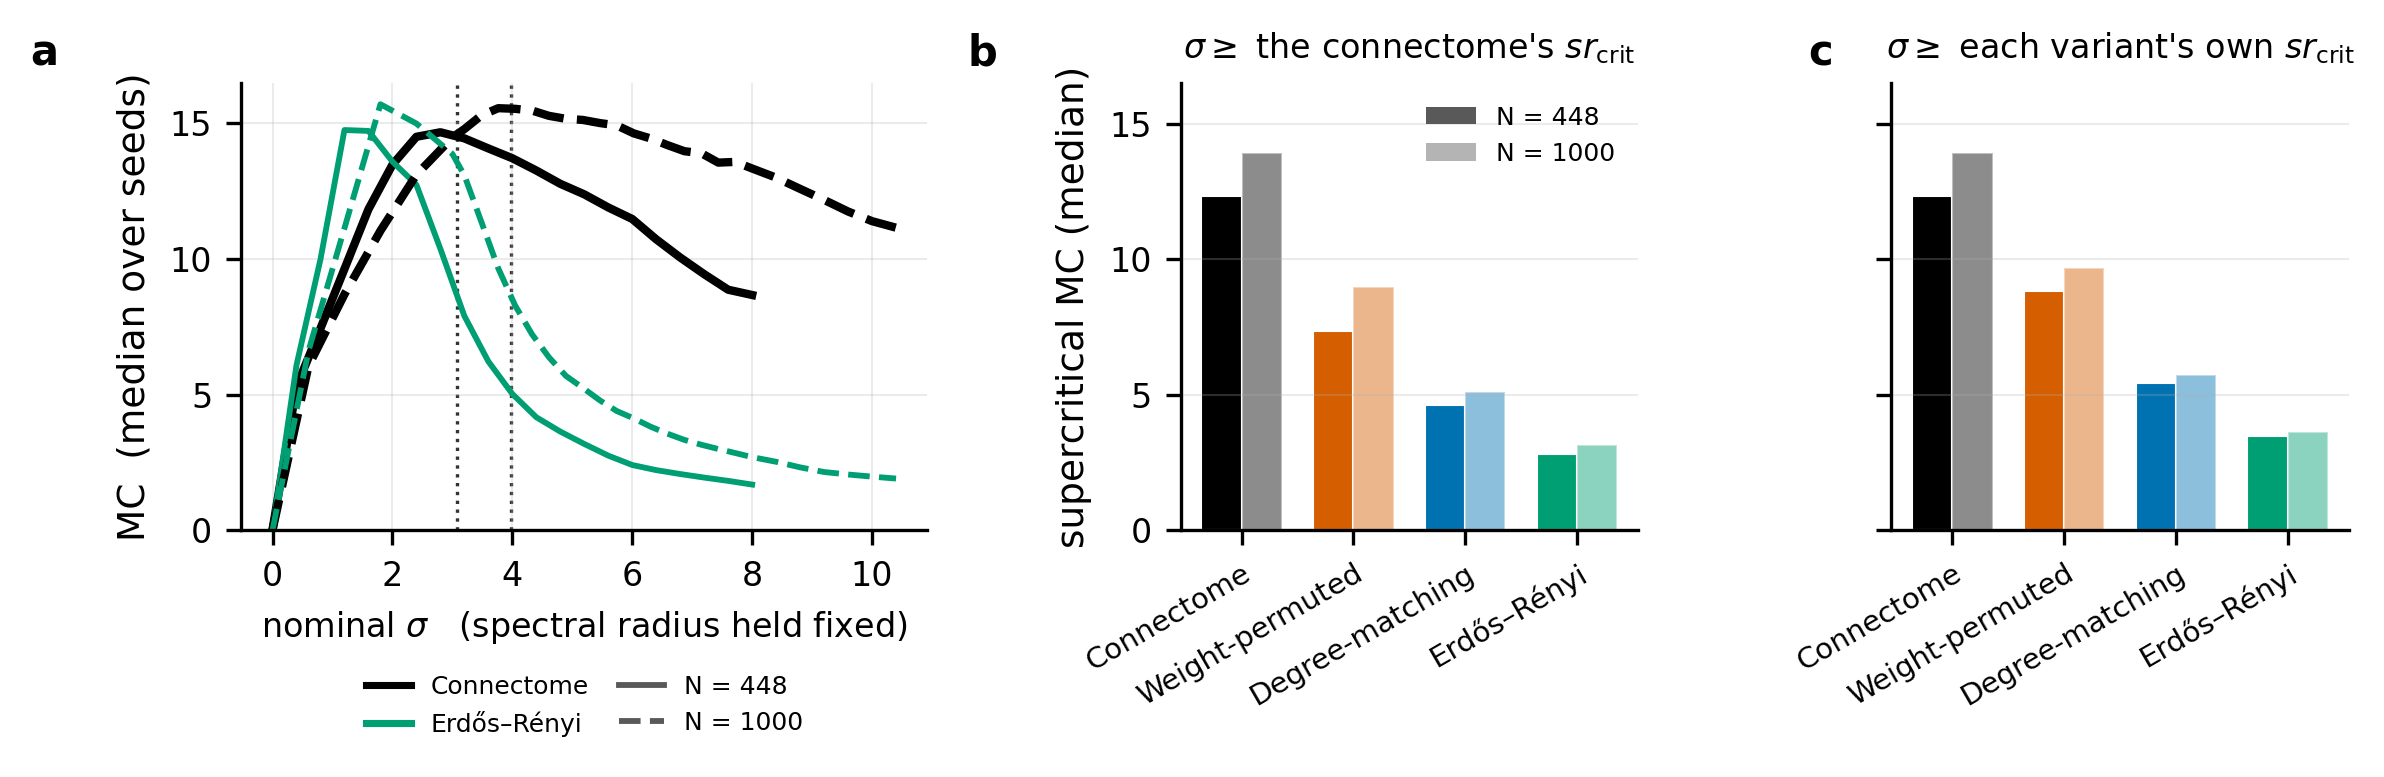
\includegraphics[width=\textwidth]{F9.png}
    \caption[The supercritical memory margin holds across a 2.2-fold change in
    $N$, under both definitions of ``supercritical'']{\textbf{The supercritical
    memory margin holds across network scale, under both definitions of
    ``supercritical''.} Memory-capacity task, non-negative weights, four
    substrates and ten seeds each; the connectome and Erdős--Rényi are drawn,
    since the panel is about scale rather than about the ladder. Run length was
    scaled from $3000$ to $6000$ to hold retained timesteps per unit near $5.5$,
    and the ridge reparameterised to scale with the Gram matrix rather than held
    at an absolute value; Appendix~\ref{app:scale} separates the two changes.
    \textbf{(a)} Median memory capacity against nominal $\sigma$ at both sizes;
    the dotted rules are the connectome's critical scale, $3.078$ at $N = 448$
    and $3.985$ at $N = 1000$. \textbf{(b)} With that threshold applied to every
    variant, the connectome to Erdős--Rényi margin is $4.40$ and $4.42$, on
    levels $12.32$ against $2.80$ and $13.93$ against $3.15$. \textbf{(c)} With
    each variant taken above its own critical scale, $3.56$ and $3.85$. Both are
    drawn because the answer depends on the filter: the margin holds either way,
    but only (b) is flat. The larger network does not escape the
    $d_{\mathrm{eff}}$ ceiling.}
    \label{fig:F9}
\end{figure}

What accounts for the retention difference has already been measured.
Chapter~\ref{chapter:act-II} found the connectome the least dominated of the four
by its common mode at every supercritical operating point, despite carrying by
far the largest Perron root, and found its Gram spectrum standing correspondingly
further clear of the readout's floor. A large gap lets the leading mode be driven
hard without the bulk of the spectrum following it, so the activity that is not
the common mode survives, and what survives clear of the floor is what the
readout can use. The retention difference in Figure~\ref{fig:F7} is that gap,
read out. That is not a larger capacity, and nothing above claims one; it is a
capacity that survives being driven away from the conditions it was measured
under.




\section{Prediction and its two failures}
\label{sec:act3-prediction-sigma}
\bigskip

A network scored on memory is handed the true signal at every step. A network
asked to generate is released after a short initialisation and runs on its own
output, so its mistakes become its own next input and accumulate, and what is
scored is how long it stays with the true signal before leaving it
(Chapter~\ref{chapter:methods}). At the operating point where each substrate is
at its best, near criticality at $\sigma = 2$, the four are not
distinguishable: the connectome's
margins over the three nulls are
$+0.28$, $-0.01$ and $+0.44$ % TIER0 2.6
Lyapunov times, none of them significant. That is the same shape as the memory
result, whose four peaks also sat within a few percent of one another. On both
demands the substrates separate away from their best operating points rather than
at them.

They separate in two different ways, and only one of them favours the connectome.
Driven well into the supercritical regime, above
$\sigma \approx 7.6$ to $8.0$, % TIER0 2.3
five of Erdős--Rényi's ten seeds settle onto a pair of states and alternate
between them, flipping from one to the other at every step and going nowhere
else. What they emit is no longer a path winding around the Lorenz attractor; it
is two points (Figure~\ref{fig:F21}a). Across the whole swept range, far above
its own critical scale, this happens to none of the connectome's ten seeds. The substrates are not being
separated here by how long they predict for, but by whether what they produce is
a trajectory at all. Five against none is significant
($p = 0.033$, % TIER0 2.3
Fisher exact), though on ten seeds per substrate the claim rests on the size and
direction of the difference rather than on the test.

\begin{figure}[ht]
    \centering
    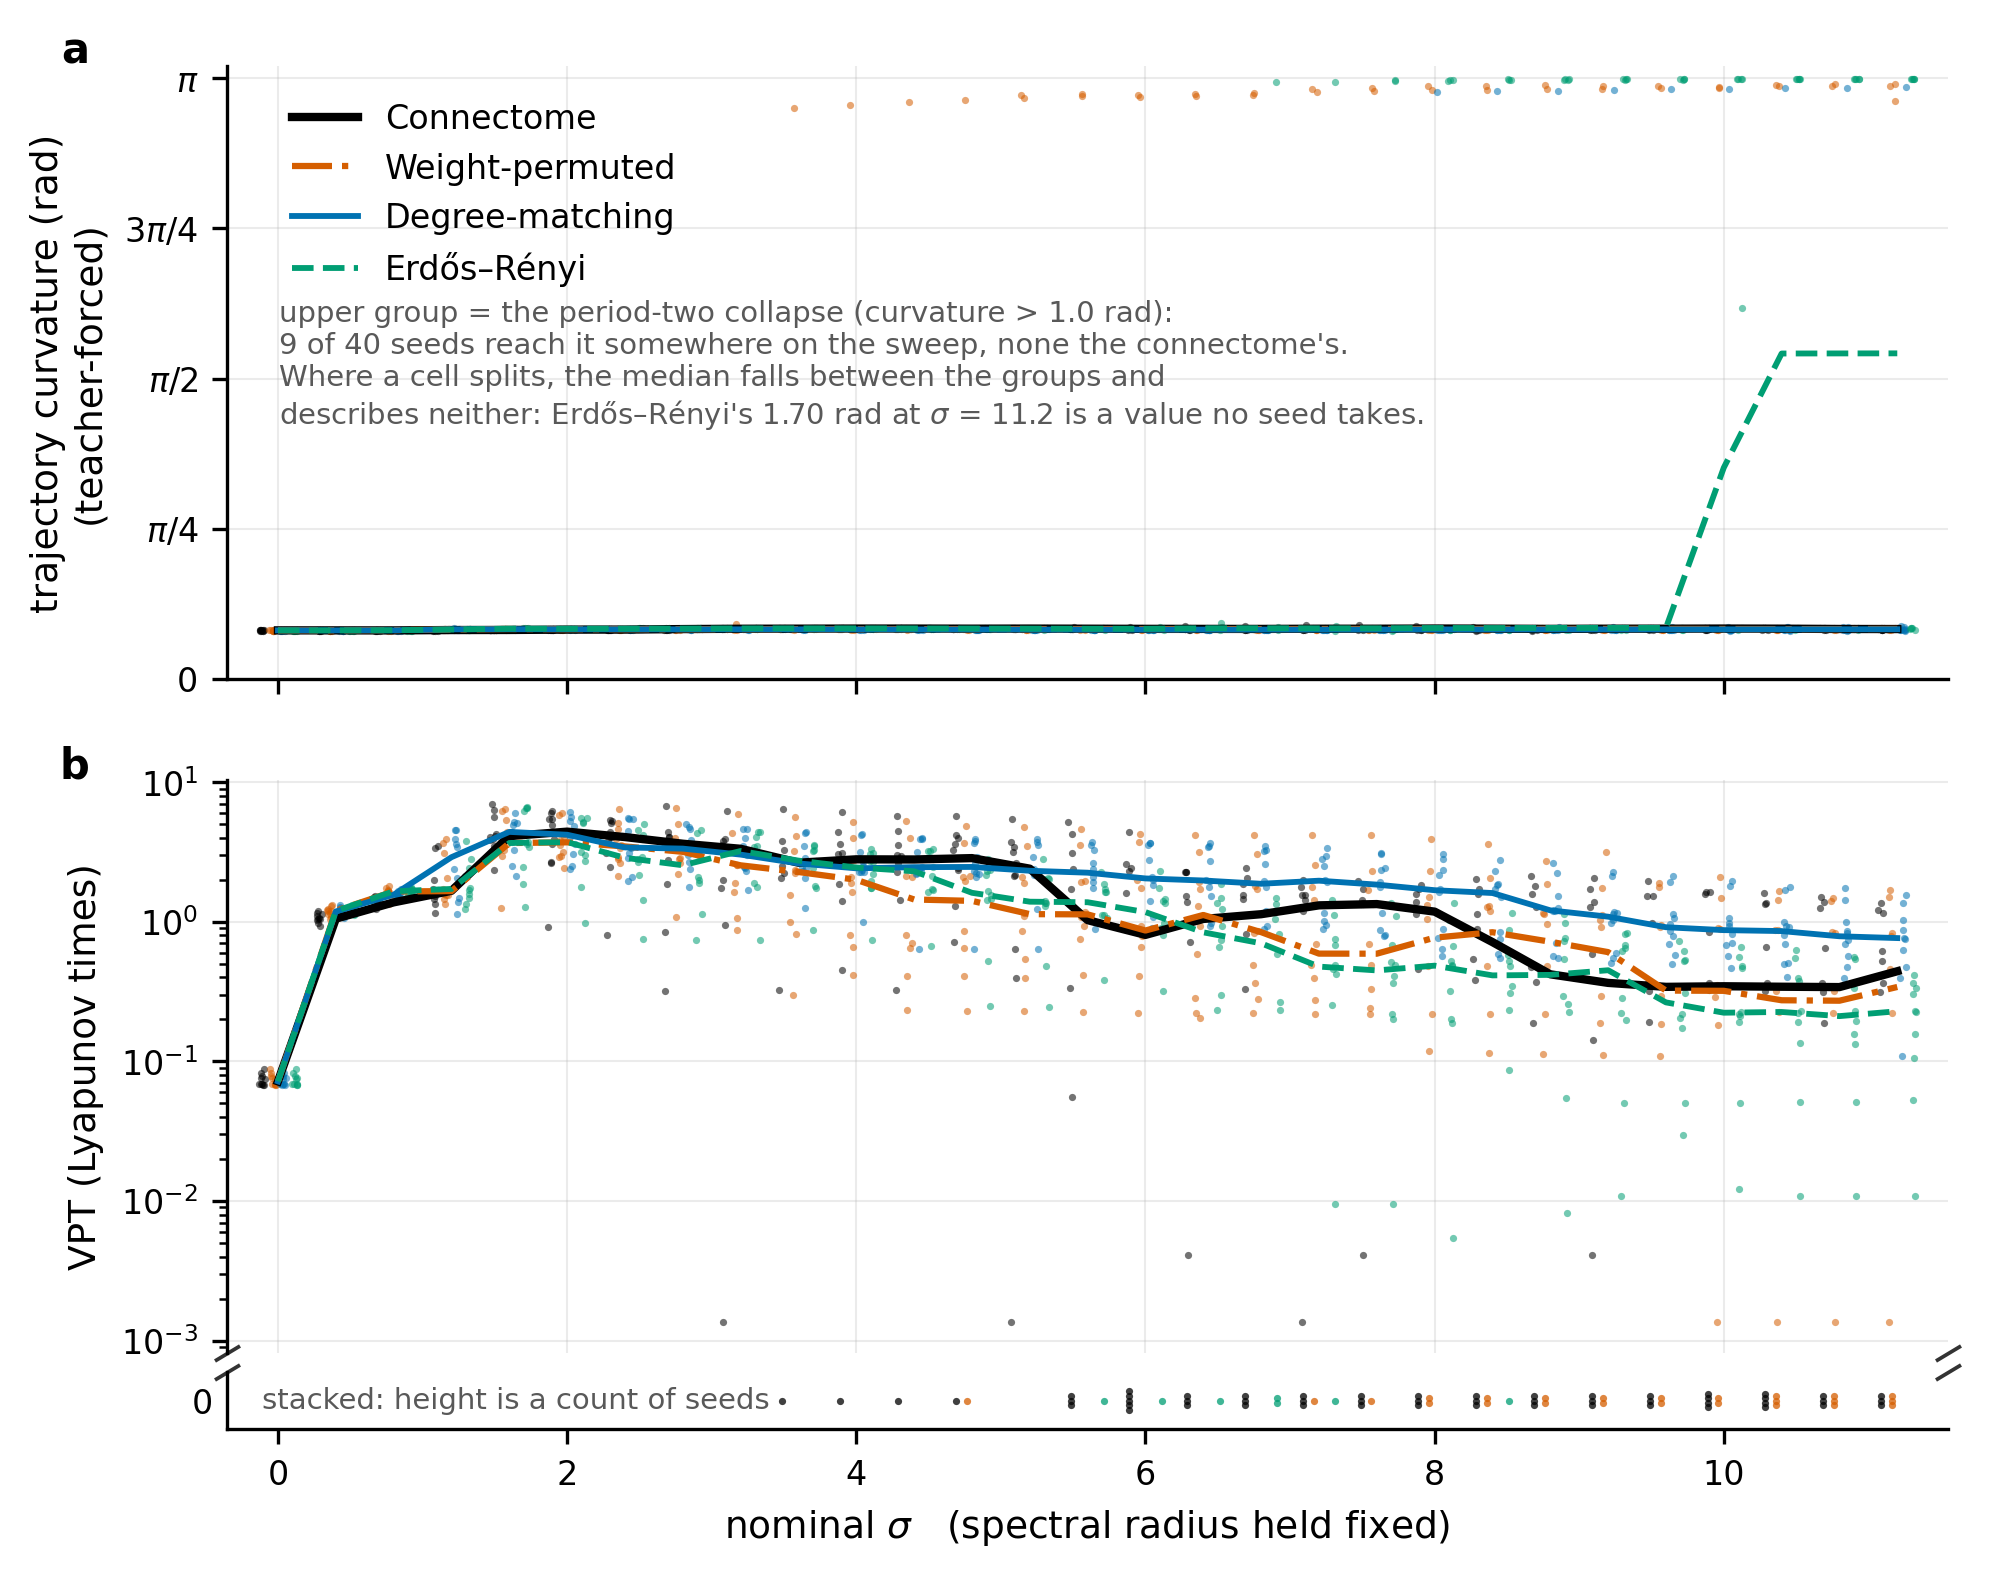
\includegraphics[width=\textwidth]{F21.png}
    \caption[Prediction falls across the operating-point sweep while trajectory
    curvature does not move]{\textbf{Prediction falls across the
    operating-point sweep while the geometry does not move.} Lorenz task,
    $N = 448$, non-negative weights, ten seeds per substrate, against nominal
    $\sigma$. Points are individual seeds and lines are seed medians.
    \textbf{(a)} Trajectory curvature, the mean angle between successive segments
    of the driven trajectory, drawn on the full $0$ to $\pi$ range so that
    flatness is not an artefact of a compressed axis. Seeds occupy two separated
    groups, one near $0.26$~rad and one just below $\pi$, and none lies between
    them. The upper group is the alternating state of the text: a two-state cycle
    reverses direction at every step, which this measure reads as an angle near
    $\pi$. Medians mislead here, and Erdős--Rényi's $1.70$~rad at
    $\sigma = 11.2$ is a value that no seed takes. \textbf{(b)} Valid prediction
    time in Lyapunov times, log axis, falling for every substrate across the same
    range; seeds scoring exactly zero are stacked on the strip below the break,
    where height reads as a count. Curvature is measured on the driven trajectory
    and prediction time on the free run. The graded loss in (b) has no
    counterpart in (a).}
    \label{fig:F21}
\end{figure}

What the connectome brings to that comparison is the same spectral gap the memory
result turned on, read from its other end. Alternation between two states is what
a network settles into when the most negative part of its spectrum grows strong
enough to dominate its own dynamics. A large gap is exactly what holds that part
far below the leading eigenvalue, so the substrate with the largest gap is the
one furthest from reaching the alternating state, and it stays furthest from it
however hard it is driven. As stated, that is an account that fits rather than
one that has been tested: every substrate compared so far has the same sign
structure, so no comparison among them can isolate it. The next section supplies
the intervention that can, and Section~\ref{sec:act3-unifying} returns to the
account itself.

The second way of failing does not favour the connectome. Counted bluntly, by how
many seeds cease to predict at all somewhere high in the sweep, the ordering
reverses: the connectome is the worst of the four, and the degree-matched null
never fails at any operating point. The two failures are separate events rather
than degrees of one, and can be shown to be: the connectome has no seed in the
alternating state anywhere, so none of the seeds on which it ceases to predict
can be a seed that collapsed. Appendix~\ref{app:second-failure} gives the
counts. What holds is the narrower statement, that the connectome resists one
specific way of failing to generate.

Neither failure shows up in the shape of the activity. The connectome's
curvature, the mean angle between successive segments of its trajectory, holds at
$0.26$~rad % TIER0 3.11
from just above criticality to the top of the sweep, while over the same range
its prediction falls roughly tenfold (Figure~\ref{fig:F21}). The measure that
carried the memory half of this chapter registers nothing here: capacity is lost
with the geometry intact. What governs that loss is left open in
Section~\ref{sec:act3-unifying}, which states the three explanations available
and eliminates each.

% Every substrate to this point has non-negative weights, so every one of them
% carries a common mode, and no contrast between them can show that the common mode
% is what any of these differences are made of. The next section stops comparing
% and starts changing the weights.





\section{Inhibition and the common mode}
\label{sec:act3-lesion}
\bigskip

Neither of the last two sections can settle its own mechanism, because every
substrate compared in them is non-negative and therefore carries a common mode: a
comparison among four networks that all share a feature cannot show that the
feature is what separates them. The account offered was that a large spectral gap
lets the leading mode be driven hard without the bulk of the spectrum following
it. If that is right, taking the common mode away should take the difference with
it. A fraction $f$ of the weights is therefore made negative, leaving the
magnitudes untouched and the topology intact, so that what changes between one
network and the next is the sign pattern and nothing else. As $f$ approaches one
half the excitatory and inhibitory contributions to each unit's input come into
balance and the all-positive leading direction has nothing left to be built from.
This is not a perturbation away from biology. Macroscale diffusion tractography
cannot represent the sign of a connection, so a non-negative matrix is what the
instrument produces rather than what cortex is, and raising $f$ asks what a
network carrying inhibition would do.\footnote{Which edges are inverted is
controlled rather than left to chance: flips are stratified by endpoint
degree, so that the inverted set has the same hub-to-periphery composition as
the graph at every $f$ and the amount of inhibition does not vary with where it
sits. Chapter~\ref{chapter:methods} gives the procedure.}

The intervention does what it was designed to do, and does it to every substrate
alike. Held at the supercritical operating point
$\sigma = 6$, % TIER0 3.7
where Section~\ref{sec:act3-memory-sigma} found the substrates furthest apart,
the common-mode amplitude falls for all four as $f$ rises, and by the time the
signs are balanced it has fallen by two orders of magnitude on every one of them
(Figure~\ref{fig:F11}a). The four curves converge as they fall, because the
connectome starts nearest the floor and has least distance to travel: the nulls
lose a feature that dominated their activity, and the connectome loses one it was
already largely free of. What the sign balance removes is therefore not something
the connectome had and the nulls lacked. It is the handicap the nulls carried and
the connectome did not.

\begin{figure}[htbp]
    \centering
    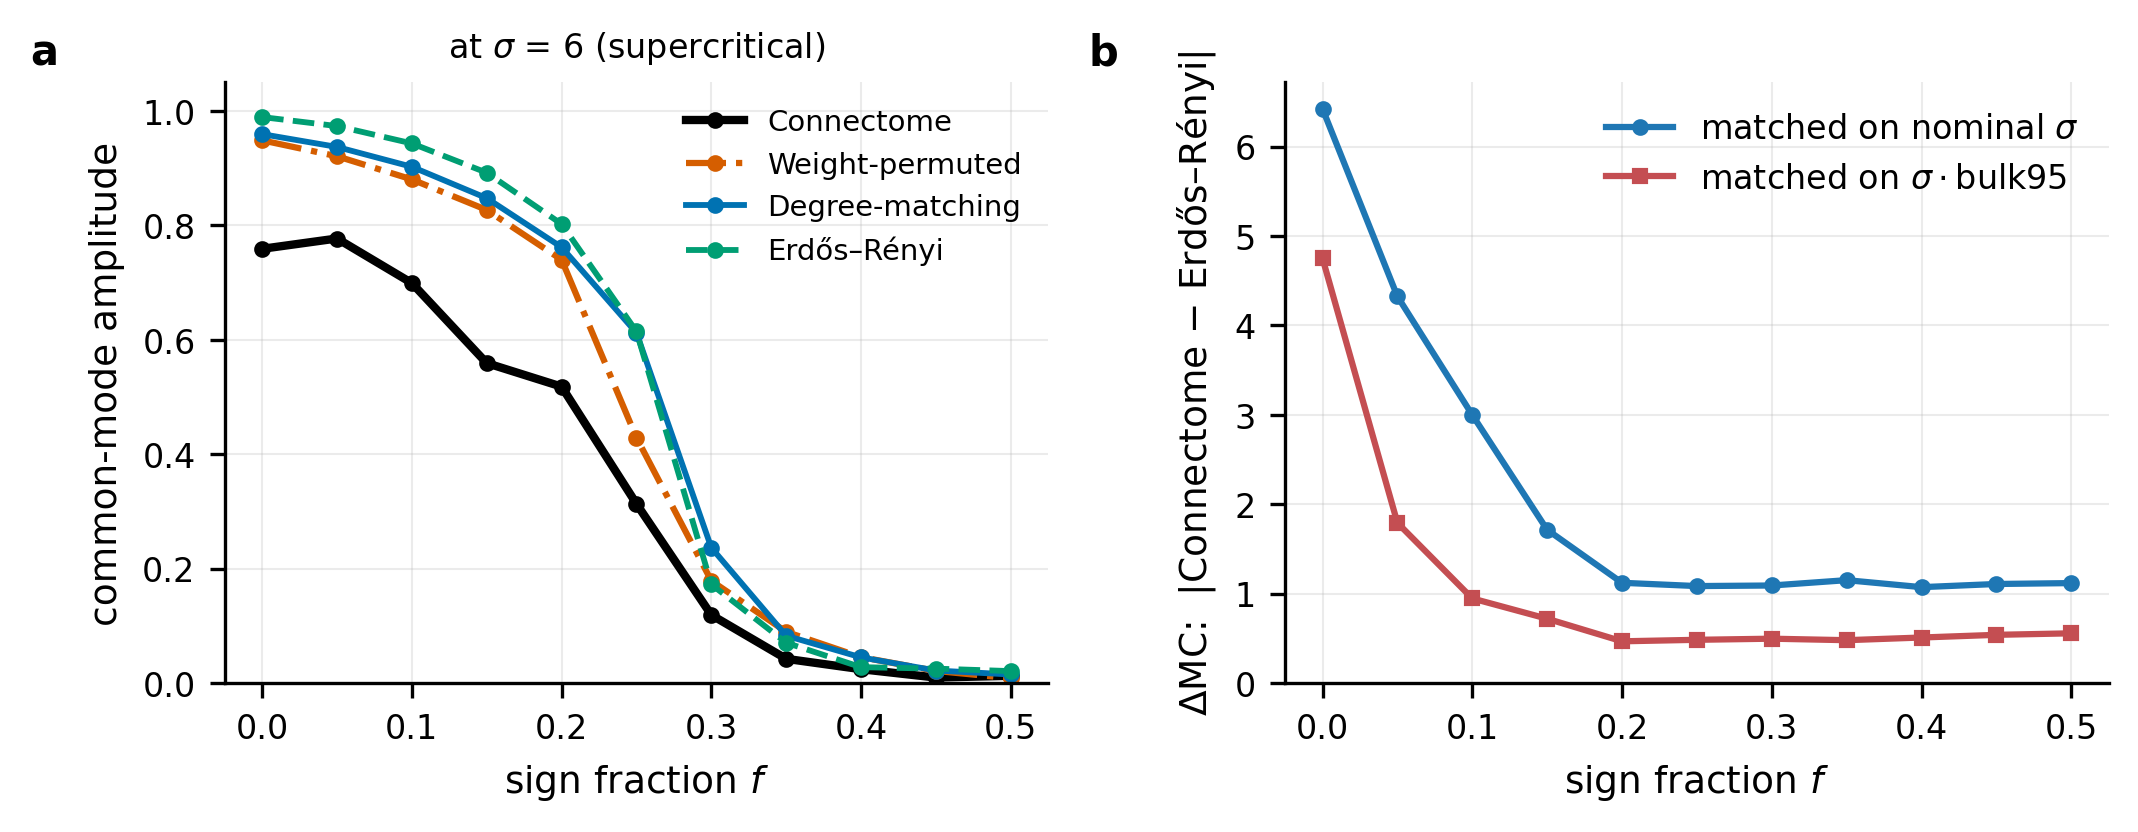
\includegraphics[width=\textwidth]{F11.png}
    \caption[Non-negativity makes memory worse for every substrate, and the
    connectome's spectral gap makes it least worse]{\textbf{The connectome does
    not make memory better; non-negativity makes it worse for every substrate,
    and the connectome's spectral gap makes it least worse.} Memory-capacity
    task, $N = 448$, ten seeds, held at the supercritical operating point
    $\sigma = 6$ throughout, against the fraction $f$ of weights made negative.
    \textbf{(a)} The common-mode amplitude, the grand mean of the state matrix
    over time and units, absolute-valued per cell before the seed median. With
    non-negative weights the nulls sit at $0.949$ to $0.989$, very nearly every
    unit pinned at one saturated value, while the connectome sits at $0.759$
    despite carrying much the largest Perron root; balancing the signs removes
    the mode entirely for every substrate. \textbf{(b)} The median absolute
    connectome-minus-Erdős--Rényi gap in memory capacity under each matching
    axis, falling from $6.42$ to $4.75$ with non-negative weights and to near
    $0.5$ under either axis by $f = 0.2$.}
    \label{fig:F11}
\end{figure}

The memory ladder goes with it, and the way it goes is the finding. The wedge
between the connectome and the nulls narrows as $f$ rises and has closed by
$f \approx 0.15$ to $0.20$. % TIER0 2.6
No substrate is harmed in the process. Supercritical memory capacity rises with
$f$ for all four, the connectome's from
$11.43$ to $14.18$ % TIER0 2.6
and Erdős--Rényi's from
$2.42$ to $13.11$ % TIER0 2.6
across the swept range at the same operating point. The advantage disappears
because the nulls catch up, and they catch up from far below because they had
much further to come. That is the prediction the common-mode account makes and
the alternatives do not: on a reading in which the connectome's weight assignment
confers some intrinsic computational property, balancing the signs should have
degraded the substrate that had the property, and instead it lifted the ones that
lacked it. The supercritical advantage is a rescue from a handicap that
non-negativity imposes on everyone, and not a capacity the connectome supplies.

The intervention also bounds how much of the ladder the bulk radius accounts for,
a question Section~\ref{sec:act3-memory-sigma} raised and could not settle.
At $f = 0$, matching the substrates on the bulk radius rather than on the Perron
root absorbs about
a quarter % A3M 2.6
of the connectome-to-Erdős--Rényi gap; once the signs are balanced it absorbs
almost none of it (Figure~\ref{fig:F11}b). It is a partial
controller, and it explains something only where there is a common mode to
explain.




\section{A second dynamical regime}
\label{sec:act3-branch}
\bigskip

Applied to prediction, the same intervention does something else entirely, and
seeing why takes one fact about what a negative weight does dynamically. Each
unit passes the weighted sum of its recurrent input, plus the drive, through a
$\tanh$. A map of that shape settles to a fixed point when its effective gain is
sufficiently positive and to a period-two orbit when the gain is sufficiently
negative, with nothing stable between the two. Non-negative weights can only
reach the first; making a fraction of the weights negative brings the second
within reach. The intervention therefore does not turn a dial. It makes a second
dynamical regime available, and a network either enters it or does not.

The activity behaves as the map says it should, and the two-group structure that
appeared at $f = 0$ in Section~\ref{sec:act3-prediction-sigma} now appears across
the whole sweep. Trajectory curvature occupies two narrow spikes with almost
nothing between them:
$98\%$ % TIER0 3.9
of cells sit either near
$0.25$~rad, % TIER0 3.9
where successive steps continue in roughly the same direction, or at
$\pi$, % TIER0 3.9
where they reverse, which is what a period-two orbit looks like measured this way
(Figure~\ref{fig:F12}). What matters for capacity is which spike a network is
in, not where on the curvature axis it sits: a single binary variable recording
the spike explains as much of the variation in prediction as the full continuous
measure does. This also withdraws a graded account that an earlier analysis of
these data supported, under which straighter trajectories predicted better;
pooled across all
cells the correlation is strong, but it is an artefact of mixing the two clusters
and it reverses in sign within either one.
Appendix~\ref{app:regime-gating} gives the regression and the reversal. Capacity
is not gated by how curved the manifold is. It is gated by which of two dynamical
regimes the manifold is in.

\begin{figure}[htbp]
    \centering
    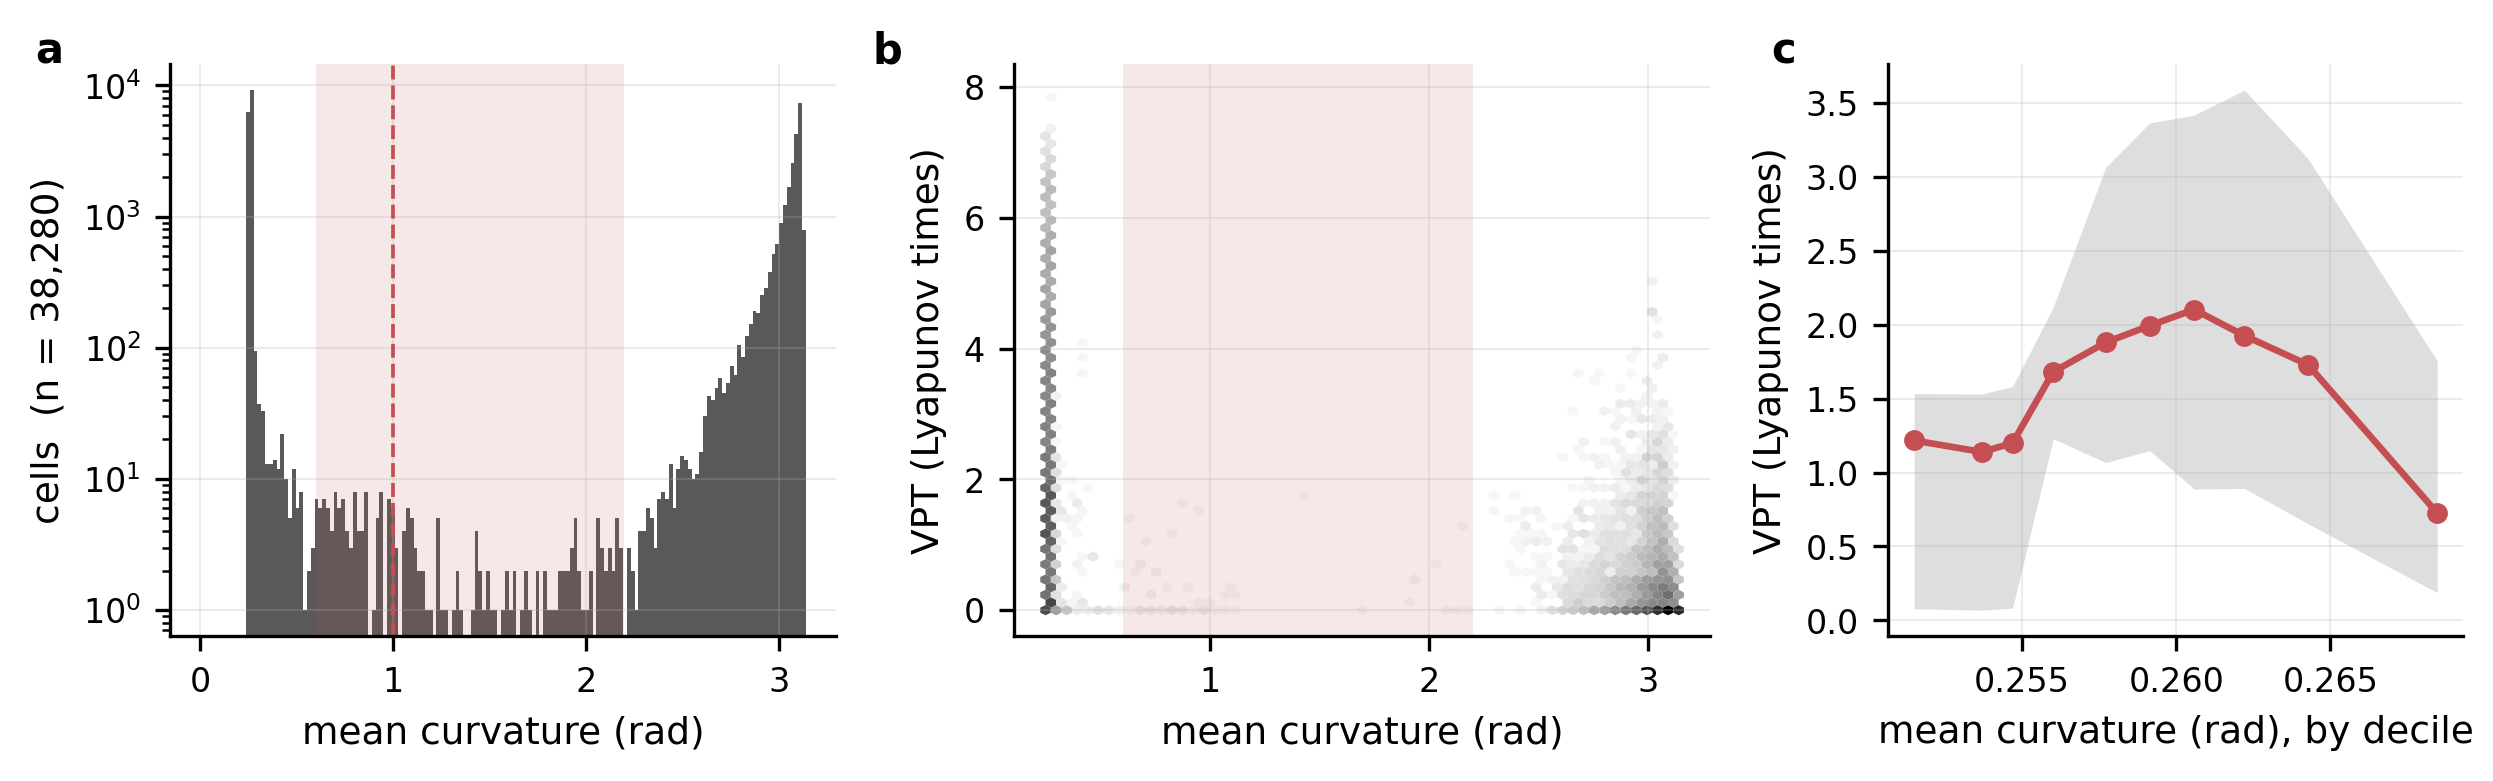
\includegraphics[width=\textwidth]{F12.png}
    \caption[Capacity is gated by dynamical regime, not graded by trajectory
    curvature]{\textbf{Capacity is gated by dynamical regime, not graded by
    trajectory curvature.} Lorenz task, $N = 448$, all four substrates over the
    full sweep in operating point and sign fraction. \textbf{(a)} Distribution of
    trajectory curvature. Two spikes, one near $0.25$~rad and one at $\pi$ where
    successive steps reverse, hold $98\%$ of cells between them; under $0.6\%$
    fall in the valley, whose midpoint at $1.0$~rad is used as a separator.
    \textbf{(b)} Prediction against curvature, coloured by cluster: a binary
    collapsed-or-not variable explains $R^2 = 0.364$ of the variance against
    continuous curvature's $0.370$. \textbf{(c)} Within the smooth cluster only,
    where the residual correlation is $+0.145$, opposite in sign to the pooled
    $-0.78$. Appendix~\ref{app:regime-gating} gives both comparisons.}
    \label{fig:F12}
\end{figure}

Which regime a network falls into, and at what sign fraction, is where weight
assignment reappears, and it is where a generative advantage opens that did not
exist before. At the near-critical operating point $\sigma = 2$ the connectome is
level with all three nulls on non-negative weights, as
Section~\ref{sec:act3-prediction-sigma} reported. A margin opens as the sign
fraction rises (Figure~\ref{fig:F13}), and at
$f = 0.25$ % TIER0 2.6
the connectome's paired advantage in valid prediction time is
$+1.71$, $+1.62$ and $+2.20$ % TIER0 2.6
Lyapunov times over the weight-permuted, degree-matched and Erdős--Rényi nulls,
the first sign fraction at which it clears all three. Across the range from
$f \approx 0.20$ to $0.25$ % TIER0 2.6
the connectome is the only substrate still predicting usefully at all, at
$1.3$ to $2.8$ Lyapunov times % TIER0 2.6
against the nulls'
$0.1$ to $0.9$. % TIER0 2.6
What licenses reading this as a property of assignment rather than of topology is
the control it clears: the weight-permuted null holds the connectome's topology
and the connectome's own weights, and changes only which weight sits on which
edge. The margin is not monotone in $f$, and it narrows considerably if what
counts as predicting is raised from not having failed outright to predicting
usefully. It is real and it is located; it is not a uniform superiority across
the sweep.

\begin{figure}[htbp]
    \centering
    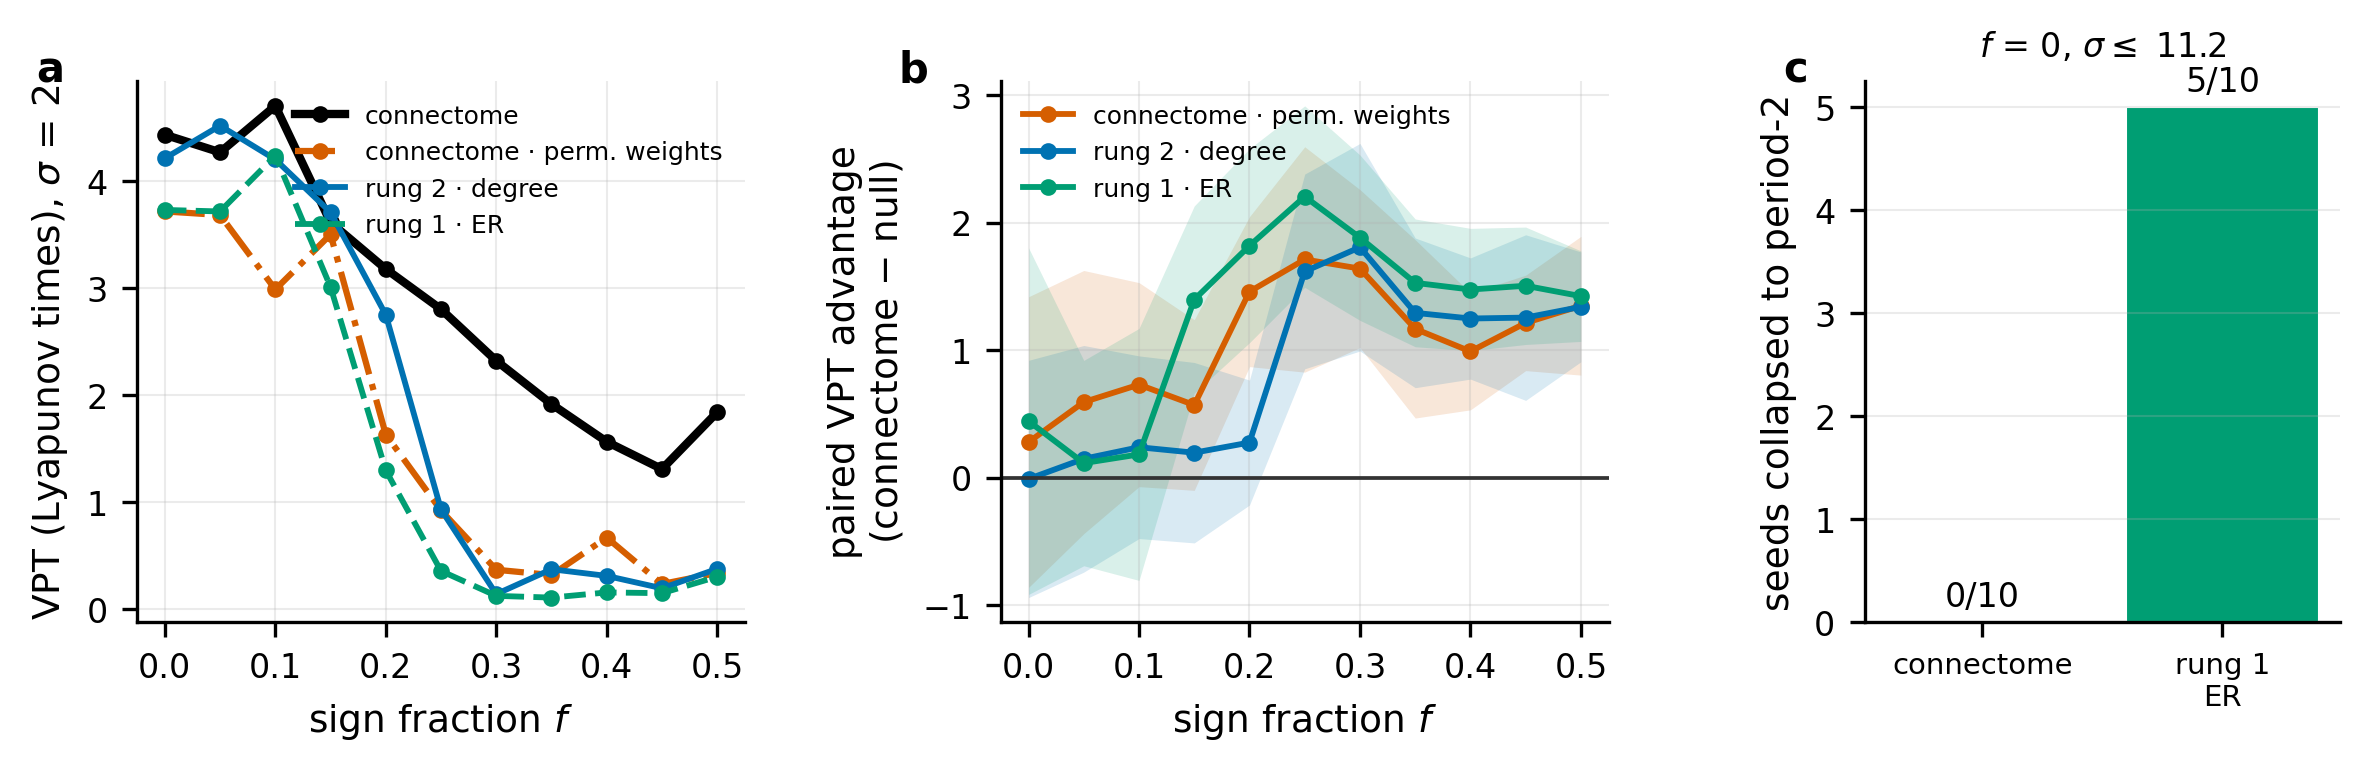
\includegraphics[width=\textwidth]{F13.png}
    \caption[A predictive advantage opens as signs are balanced, and clears the
    assignment control]{\textbf{A generative advantage opens as signs are
    balanced, and clears the assignment control.} Lorenz task, $N = 448$, ten
    seeds, at the near-critical operating point $\sigma = 2$ throughout, against
    the sign fraction $f$. \textbf{(a)} Median valid prediction time per
    substrate. \textbf{(b)} The connectome's advantage over each null, paired
    within seed so that every comparison shares its input weights and input
    series. None of the three margins is significant on non-negative weights; all
    three are cleared first at $f = 0.25$, and the margin is smaller at
    $f = 0.50$ than at its best, so it is not monotone in $f$. \textbf{(c)} At
    $f = 0$ and far above criticality, seeds collapsing to a period-two orbit:
    five of ten for Erdős--Rényi and none of ten for the connectome
    (Section~\ref{sec:act3-prediction-sigma}). This panel covers only the two
    substrates the boundary capture contains.}
    \label{fig:F13}
\end{figure}







% \newpage

\section{One property, two demands}
\label{sec:act3-unifying}
\bigskip

The two demands read one property with opposite sign, and it is the property
Chapter~\ref{chapter:act-I} measured. The connectome's spectral gap is the
largest on the ladder: its Perron root stands
$3.08$ % TIER0 3.1
times clear of its bulk edge against Erdős--Rényi's
$1.81$ % TIER0 3.1
(Section~\ref{sec:act1-spectrum}). Expressed the other way up, everything
beneath the Perron root sits proportionally nearer the origin, and because these
matrices are symmetric at $f = 0$ that includes the negative end: the most
negative eigenvalue reaches
$0.33$ % TIER0 3.9 [VERIFY quantity]
of the leading one for the connectome against Erdős--Rényi's
$0.55$. % TIER0 3.9 [VERIFY quantity]
So stated, the gap is a distance to the second branch of the map of
Section~\ref{sec:act3-branch}. A network settling toward the fixed-point branch
produces smooth trajectories, which is what a closed loop needs in order to keep
generating; the same settling synchronises the units, so they stop doing
different things and the readout dimensions a linear map could have used are
wasted. What helps prediction is what costs memory.

Put both demands on one grid and the reversal is visible directly
(Figure~\ref{fig:F22}). Memory improves as
the sign fraction rises, and the improvement is an ordering of the supercritical
decay: steepest on non-negative weights and nearly flat once a quarter of the
weights are negative, which is the rescue of Section~\ref{sec:act3-lesion} shown
as a family of curves rather than asserted. Prediction orders the other way, its
tallest peaks belonging to the lowest sign fractions and the sign-balanced curves
reaching zero well before the end of the sweep. What divides the two is not how
far back each reaches into the past but whether the network runs on its own
output, which is what makes the regime it settles into consequential in one case
and harmless in the other.

\begin{figure}[h!]
    \centering
    
\includegraphics[width=\textwidth]{figures/fig_frontier_absolute.png}
    \caption[Memory and prediction respond to the sign fraction in opposite
    directions]{\textbf{Memory and prediction respond to the sign fraction in
    opposite directions, on every substrate.} $N = 448$, four substrates and ten
    seeds each, plotted against nominal $\sigma$; curves are seed medians, coloured
    by the fraction $f$ of weights made negative, from $f = 0$ (non-negative, dark)
    through $f = 0.5$ (sign-balanced, light). Columns are the four-substrate ladder.
    Dotted rules mark each substrate's own critical scale on its non-negative matrix,
    and shading marks the range of $\sigma$ over which most seeds sit at the metric's
    floor. \textbf{(a)--(d)} Memory capacity: the total input variance a linear
    readout recovers across all delays, higher being better, peaking between $14.3$
    and $15.5$. \textbf{(e)--(h)} Valid prediction time: how long a released network
    stays with the true Lorenz trajectory, in Lyapunov times, higher being better.
    Peaks reach $4.4$ for the connectome and degree-matching and $3.7$ for the other
    two; the sign-balanced curves peak below $1.8$ and reach zero from
    $\sigma \approx 4$ onward. Vertical scales are shared within each row and are not
    comparable between rows.}
    \label{fig:F22}
\end{figure}

The memory advantage of Section~\ref{sec:act3-memory-sigma} and the predictive
advantage of Section~\ref{sec:act3-branch} are therefore not two findings that
happen to point the same way. They are one structural property measured by two
demands that want opposite things from it, and what in that account is measured
should be separated from what is inferred. The measurements are the two-state
distribution of trajectory curvature, the fact that a binary regime variable
explains nearly as much of prediction as the full geometry does, the ordering of
common-mode amplitude across substrates, the operating points at which
free-running trajectories collapse, and the opposed responses of the two demands
to the sign fraction. The inference is that a single account, built on where a
substrate's leading eigenvalue sits relative to the rest of its spectrum,
generates all of it. That account is consistent with everything measured here, and it is not a
derivation: nothing here shows that the two readouts must follow from the one
cause, only that they do wherever this work has looked.

The account also has a boundary, and it runs through the middle of this chapter
rather than around its edge. Capacity gated by dynamical regime is a statement
about networks carrying negative weights, and not about the substrate the
instrument actually produces. A non-negative matrix has no dominant negative
eigenvalue to flip, so the second branch is unreachable and there is no switch to
be gated by, and the quantity the mechanism is built on registers nothing: this
is the flat curvature Section~\ref{sec:act3-prediction-sigma} measured against a
tenfold loss of prediction. Three explanations were available and each fails.
Not geometry, which does not move. Not the
effective spectral radius, which the transition does not track: where prediction
is being lost it stands two orders of magnitude below its own largest value and
on the descending branch of its own
curve. % TIER0 3.11 [VERIFY subject clause]
And not memory, since at $\sigma = 6$ the connectome holds
$11.43$ against Erdős--Rényi's $2.42$ % TIER0 3.11
in memory capacity and a \emph{lower} valid prediction time,
$0.81$ against $1.18$. % TIER0 3.11
Whatever governs prediction on non-negative weights, this work has not found it,
and no part of the account above should be read as covering it.

Read from the biological side, the two demands say something neither says
alone. Neither is served best by a network tuned to one point, and what the
connectome supplies on both is the width of the region in which it does not fail:
memory carried further from its optimum, and prediction sustained further into
inhibition than any null reaches. A structure organised that way is not one that
computes best. It is one that needs less precise tuning in order to compute at
all, which is the reading Chapter~\ref{chapter:discussion} returns to.
 
    \chapter{Act IV: Structure Recovers Function}
\label{chapter:act-IV}
    \chapter{Discussion \& Future Work}
\label{chapter:discussion}


    \chapter{Conclusion}
\label{chapter:conclusion}
\bigskip




    
    % Bibliography with numeric style
    \printbibliography[title=References]
    \addcontentsline{toc}{chapter}{References}

    % %% Add bibliography
    % \printbibliography[heading=bibintoc,title=References]
    
    % __ Appendix ___
    \appendix
    \chapter{Appendix: Supplementary Material}
\label{appendix:supplementary}


\section{The wider substrate ladder}
\label{app:wider-ladder}
\bigskip

Section~\ref{sec:act1-assignment} rests the weight-assignment claim on the
weight-permuted control and reports two further rungs as corroboration. Their
values are here. The clustering-preserving and modularity-preserving rewires
each hold fixed everything the degree-preserving rewire does and one further
property of the topology besides; 
the random gaussian rung is included for completeness and takes no part in any
comparison, since it is not a rung of the criticality-matched ladder and matches
the connectome's edge count only in expectation.

Holding progressively more of the connectome's topology fixed recovers none
of what the assignment supplies. At $N = 448$ the strongest null of all six is the
clustering-preserving rewire at
2.081, % TIER0 3.1(b)
above every rung the figures draw, and the connectome's margin over it is
1.479-fold; % TIER0 3.1(b)
at $N = 1000$ Erdős–Rényi remains the strongest and the margin is
1.635-fold. % TIER0 3.1(b)
The separation therefore survives at both parcellations against every null
available, but its size depends on which null set it is measured against, and it
is quoted here with that set named. On $|\lambda_1|$ all three additional rungs
sit inside the null band at both scales, so the reading of
Chapter~\ref{chapter:act-I} is unchanged: a large Perron root over a bulk close
to everyone's.

These three rungs are not part of the four-substrate ladder. They appear in no
figure of Chapter~\ref{chapter:act-I}, the published spreads in
Table~\ref{tab:act1-ladder} are the ladder's and are not recomputed across the
wider set, and the near-identity of the absolute bulks stated at $N = 448$ is a
statement about the four.


\begin{table}[ht]
    \centering
    \caption[The three off-ladder substrates]{\textbf{The three substrates
    outside the four-rung ladder.} Aggregation and units as
    Table~\ref{tab:act1-ladder}: medians over ten seeds, raw units of $\mathbf{W}$,
    absolute bulk the product of the medians. All three are resampled at every
    seed, so unlike the connectome the two aggregation orders differ on every
    row, and only the product of medians satisfies the gap-ratio identity.}
    \label{tab:act1-offladder}
    \begin{tabular}{lrrrr}
        \toprule
        substrate & absolute bulk & $|\lambda_1|$ & $\mathrm{bulk95}$ & gap ratio \\
        \midrule
        \multicolumn{5}{l}{\emph{$N = 448$}} \\
        random gaussian & 0.0593 & 0.1104 & 0.5374 & 1.861 \\ % TIER0 3.1(b)
        clustering rewire & 0.0582 & 0.1212 & 0.4806 & 2.081 \\ % TIER0 3.1(b)
        modularity rewire & 0.0598  & 0.1167 & 0.5123 & 1.952 \\ % TIER0 3.1(b)
        \midrule
        \multicolumn{5}{l}{\emph{$N = 1000$}} \\
        random gaussian & 0.0558 & 0.1357 & 0.4113 & 2.432 \\ % TIER0 3.1(b)
        clustering rewire & 0.0581 & 0.1377 & 0.4218 & 2.371 \\ % TIER0 3.1(b)
        modularity rewire & 0.0604 & 0.1353 & 0.4462 & 2.241 \\ % TIER0 3.1(b)
        \bottomrule
    \end{tabular}
\end{table}

% full substrate family adjacency matrices
\begin{sidewaysfigure}
    \centering
    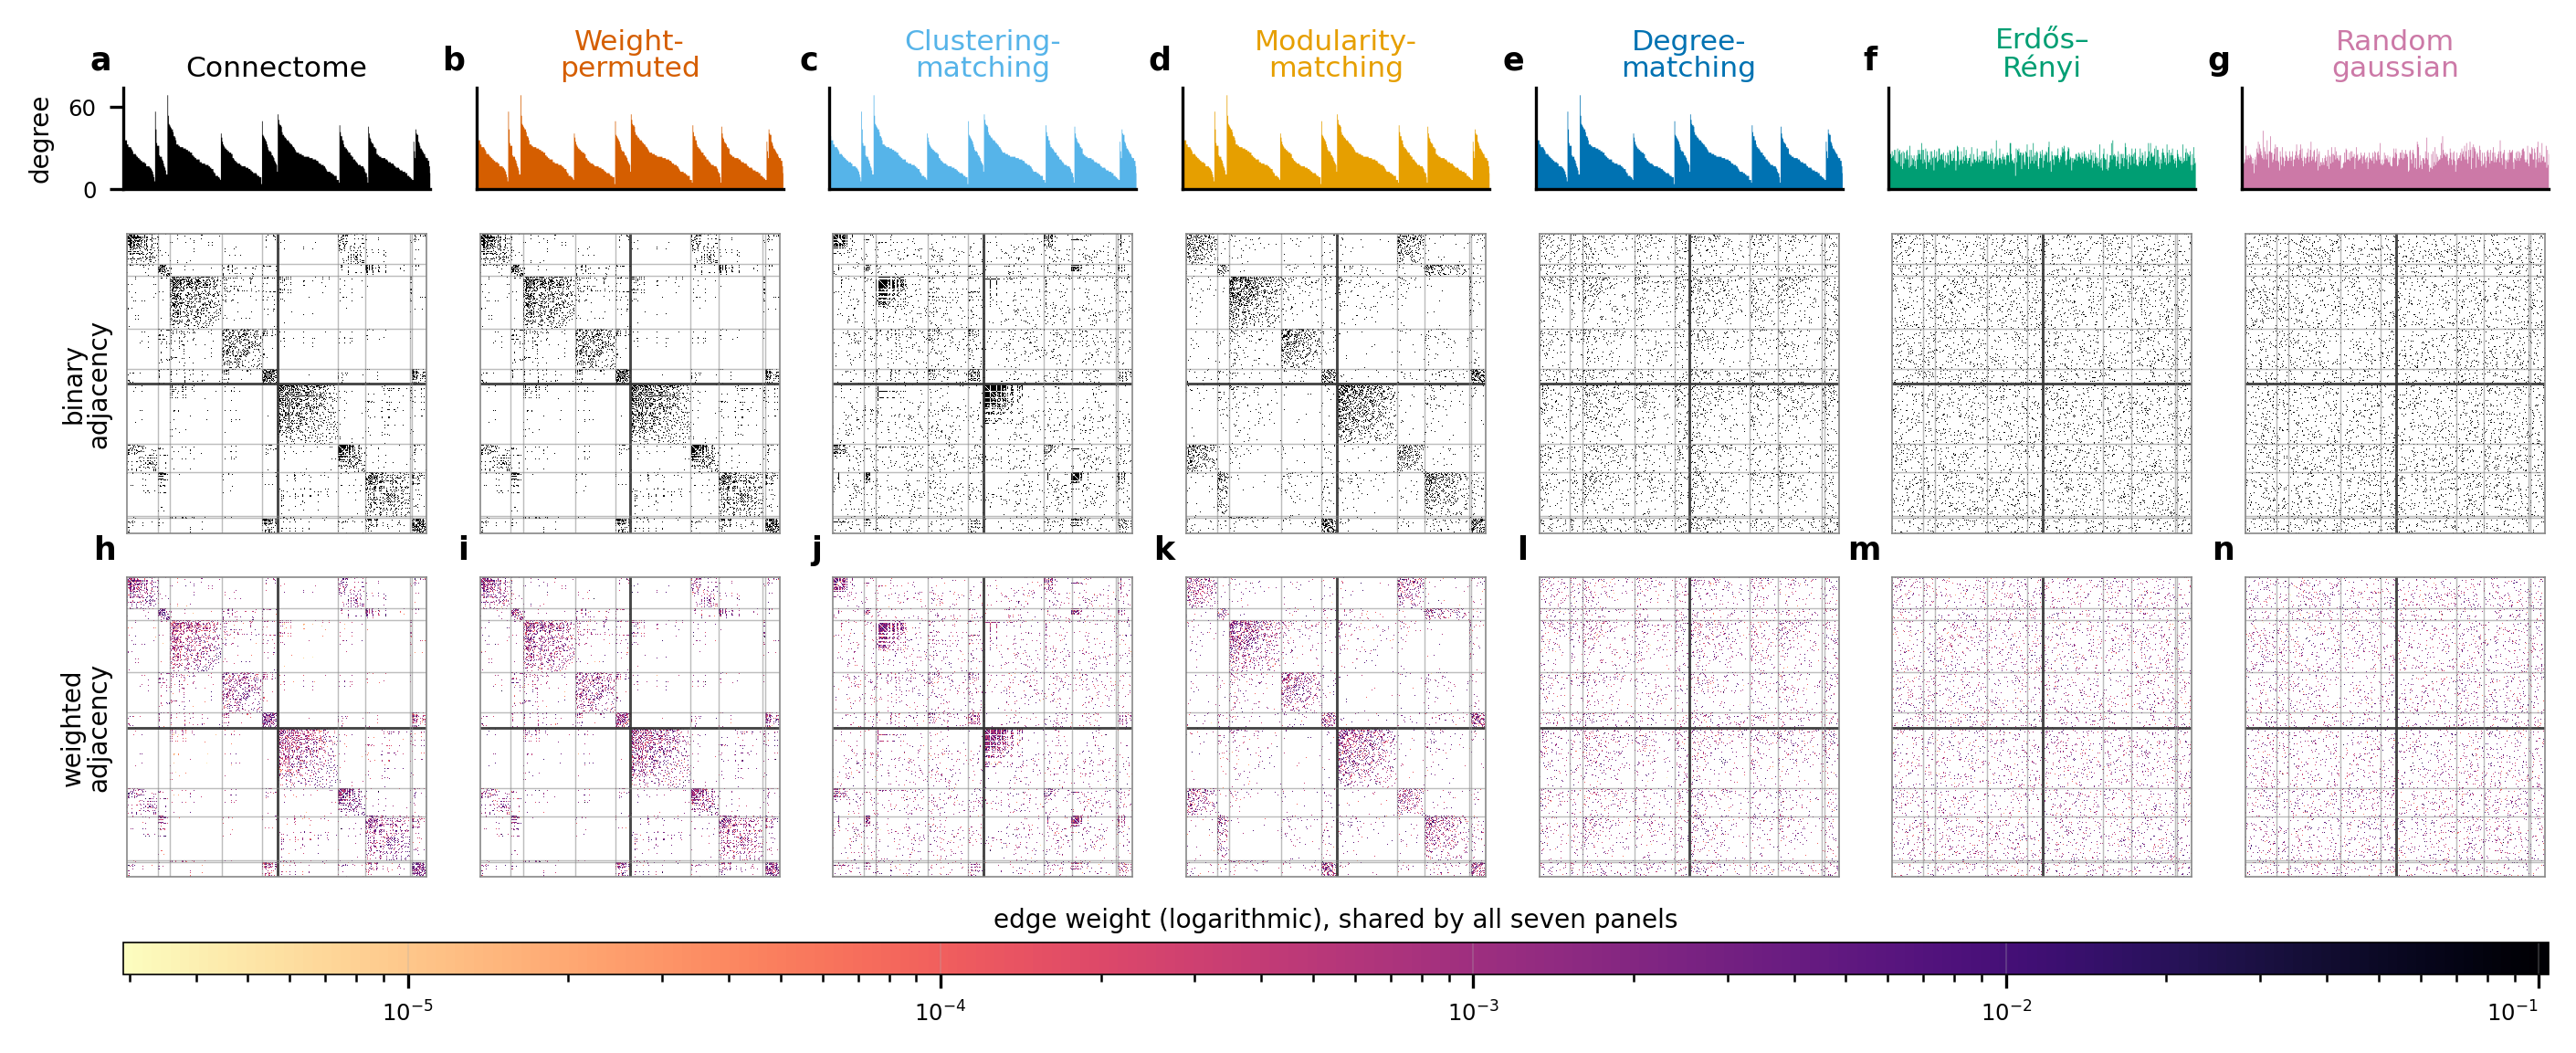
\includegraphics[width=0.95\textheight]{S4.png}
    \captionsetup{font=small}
    \caption[The full substrate family, as graphs]{%
    \textbf{The full substrate family.} All seven substrates, drawn under the
    node ordering of Figure~\ref{fig:F19}: hemisphere, then community, with
    communities detected once on the connectome and reused throughout.
    \textbf{Top row} binary adjacency with the degree marginal above each panel;
    \textbf{bottom row} weighted adjacency, all seven on one logarithmic colour
    scale. Columns run in the order of
    Table~\ref{tab:methods-preservation}, most preserved first. The
    criticality-matched ladder Chapter~\ref{chapter:act-I} draws is the
    connectome, the weight-permuted control, the degree-preserving rewire and
    Erdős–Rényi, in columns one, two, five and six; the clustering-preserving
    and modularity-preserving rewires in columns three and four each hold fixed
    everything the degree rewire does and one further property of the topology
    besides, and the random gaussian rung in column seven fixes only the node
    count and the expected density, so it is the one substrate whose edge count
    varies between seeds. Every randomised substrate takes its weights from the
    connectome's own multiset, so all seven are non-negative. This figure shows
    what the substrates look like and makes no comparison among them: the ladder
    statistics of Table~\ref{tab:act1-ladder} are the ladder's and are not
    recomputed across this set, and the spectra of the three additional
    substrates are in Table~\ref{tab:act1-offladder}. Randomised substrates are
    drawn at the seed used throughout this chapter.}
    \label{fig:S4}
\end{sidewaysfigure}





\section{A pre-registered test of one mechanism}
\label{app:mechanism}
\bigskip

Chapter~\ref{chapter:act-I} localises the spectral gap to weight assignment and
claims no mechanism for it. One candidate mechanism was specific enough to
test, and was tested. The prediction, its falsifier and the decision rule were
committed before any of the analysis ran.

The candidate is the weighted rich club. For a symmetric non-negative matrix
the Perron root is the maximum of the Rayleigh quotient over non-negative
vectors, so heavy weights on edges sharing endpoints reinforce one another in
it while scattered heavy weights do not. If the connectome's heavy edges ran
between its hubs they would share endpoints, and a weight permutation, which
holds the graph and the multiset fixed, would destroy that arrangement and the
Perron root with it.

Three predictions were registered. Edge weight would correlate positively with
endpoint degree product in the connectome and at zero in the control; the
heaviest edges would carry a larger fraction of the Perron root in the
connectome than in the control; and the ratio of maximum node strength between
them would be smaller than their Perron ratio, excluding a single dominant node
as the explanation.

The first fails, in the direction opposite to the prediction, and
Figure~\ref{fig:S3} is the measurement. The second was posed on a fraction of
each substrate's own Perron root, which divides by the one quantity these
substrates differ in, so it cannot be read: the same normalisation this thesis
retracts in Section~\ref{sec:act1-assignment}. The third fails and
leaves an account standing rather than excluding one. Weight assignment
concentrates node strength: the connectome's maximum node strength is
2.54 times % TIER0 3.14
the control's while its Perron root is 1.65 times, % TIER0 3.14
on identical mean strength. That is a candidate this thesis does not test. It
was not the registered hypothesis, it arrives from a measurement designed to
exclude it rather than to examine it, and adopting it here would be the
post-hoc move the registration exists to prevent.

The registered decision rule returned equivocal, so nothing in the claims
register changed and the limit stated in
Section~\ref{sec:act1-assignment} stands as written.

\bigskip
\begin{figure}[ht]
    \centering
    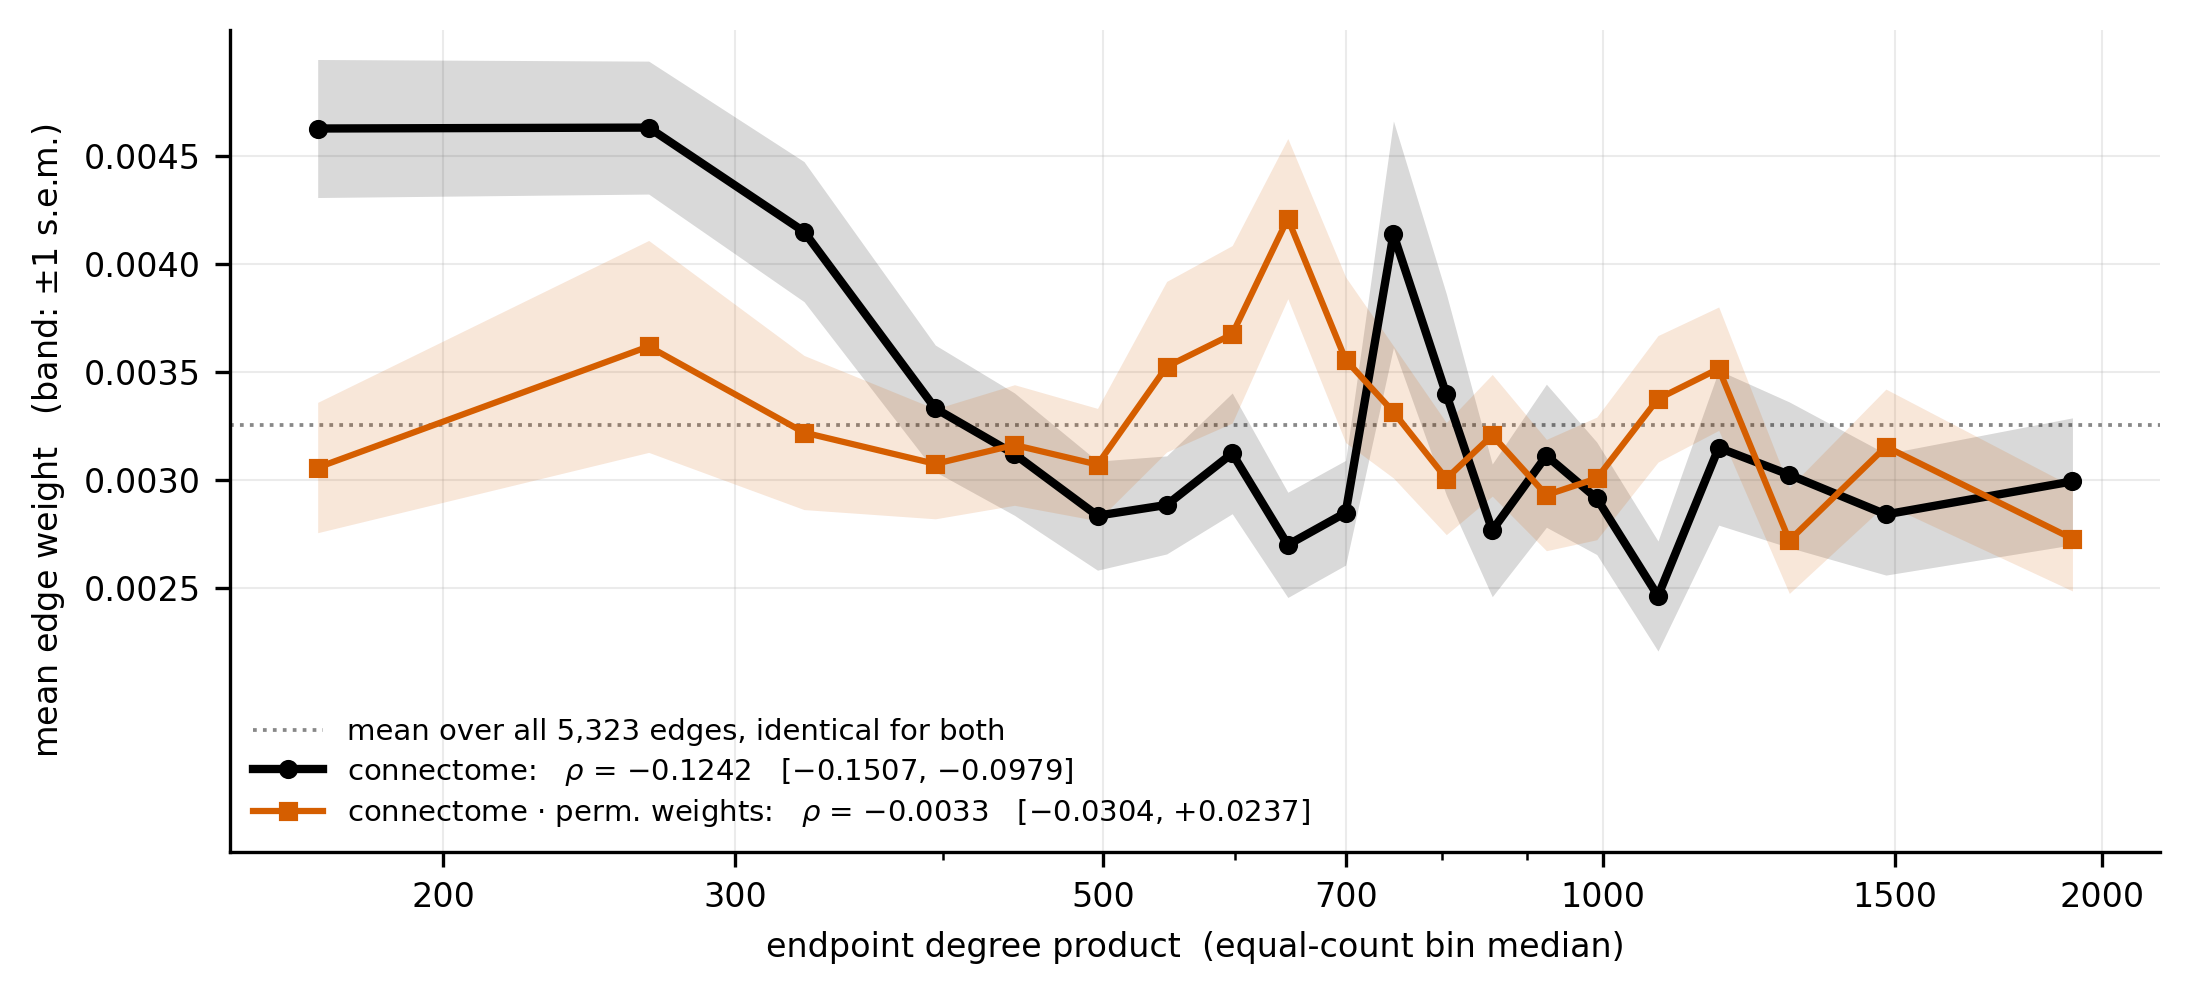
\includegraphics[width=\textwidth]{S3.png}
    \caption[The connectome's heavy edges avoid its hubs]{%
    \textbf{The connectome's heavy edges run between its lower-degree parcels.}
    Mean edge weight against the product of the two endpoints' binary degrees,
    in twenty equal-count bins cut on the connectome's products so that both
    substrates bin identically. The weight-permuted control holds the graph and
    the weight multiset fixed, so any trend it shows is sampling noise, and it
    shows none: Spearman
    $-0.0033$, % TIER0 3.14
    with a bootstrap interval covering zero. The connectome's trend is negative,
    Spearman $-0.1242$ % TIER0 3.14
    with an interval excluding zero. A weighted rich club would put the trend
    the other way. 
    Ten thousand edge resamples, 95\% percentile intervals, $N = 448$. % TIER0 3.14
    }
    \label{fig:S3}
\end{figure}




\section{Sign selects the basis}
\label{app:sign-basis}
\bigskip
% Carries A2.3, the one claim in the act that is deliberately NOT a
% contribution. Confirmatory of Krauss 2019. Moved here from chapter 5 as
% secondary material bounding a claim made there; F5 moves with it.
% Sources: fact sheet 11, plus audit item 23 for the nested coverage.
% FORBIDDEN here (sheet 11): "the manifold lives in low-frequency graph
% harmonics"; any ladder reading of this capture; "sign-gating of the manifold
% transition is a new result"; "balancing the signs improves the
% representation"; quoting the capture values as evidence of how much structure
% the bases hold; treating this as a result about the sign fraction f, which is
% chapter 6's intervention; "compact bulk"; any graded curvature account.

Section~\ref{sec:act2-perron} found the low-frequency harmonics of the graph
Laplacian standing well above chance among the connectome's fluctuations while
the dominant eigenvectors of $\mathbf{W}$ fell below it. That is easy to read as a fact
about the connectome, and it is not. It is a fact about non-negativity, and the
way to show as much is to remove the non-negativity and leave everything else
where it is.

With non-negative weights the leading eigenmodes of $\mathbf{W}$ have been absorbed into
the rank-one term of Equation~\ref{eq:gram-split}, which leaves the fluctuations
to be organised by something other than the dynamical modes themselves.
Balancing the signs of the weights destroys the Perron guarantee, so there is no
dominant common mode for those eigenmodes to be absorbed into, and the
prediction is simply that they should come back.

They do. Table~\ref{tab:app-basis} repeats the basis comparison across three
weight conditions on one substrate: the empirical weights used throughout
Chapter~\ref{chapter:act-II}, the same magnitudes with their signs balanced, and
gaussian weights. The ordering of the two structural bases swaps between the
first condition and the other two, it swaps in the same direction on all three
tasks, and the topology never changes: the same graph, the same edges, and in
the first two conditions the same weight magnitudes, with only the signs
redistributed. Figure~\ref{fig:F5} draws the clearest of the three cases across
the whole range of $k$.

The swap is the measurement, and the magnitudes are not. On the all-positive
substrate neither basis holds much of anything, the whole range across bases and
tasks running
0.04 to 0.17, % TIER0 3.12
so the fluctuations are not being shown to live in graph harmonics. Which basis
leads is what the comparison establishes; how much either one captures is a
separate question, and the answer to that one is not much.

That low capture is what the other probe predicts. Supercritically the readout
has around 413 % TIER0 3.6
of 448 directions available to it on this substrate, so the fluctuations are
spread over hundreds of directions and no ten-vector basis should be able to
hold them. The agreement runs to the other end as well: where a condition's
effective rank is low the capture is high, reaching
0.886 % TIER0 3.12
for the gaussian weights on NARMA-10. Two probes measuring different things on
different bases agree about which conditions spread their activity widely, and
neither was fitted to the other.

Two limits. The first is priority. That weight sign composition gates which
basis the fluctuations occupy is largely pre-empted by Krauss et
al.~\cite{krauss2019weight}, and it is reported here as confirmatory; the
counting argument of Section~\ref{sec:act2-counting} needs the basis established
first. The second is scope. The signed and gaussian conditions
are weight families compared side by side. Nothing has been done to the
connectome to produce them, and the question of what happens when negative
weights are introduced as an intervention on the real substrate belongs to
Chapter~\ref{chapter:act-III}, where it is used to remove the common mode and to
check whether its consequences go with it.

\begin{table}[ht]
    \centering
    \caption[Which structural basis the fluctuations occupy]{\textbf{Which
    structural basis the fluctuations occupy, across three weight conditions and
    three tasks.} Fraction of time-centred state variance held by the leading
    ten vectors of each basis, connectome substrate,
    $N = 448$, % TIER0 2.1
    medians over ten seeds. Each condition is measured at its own supercritical
    operating point, 3.0526, 2.5263 and 1.2632 % A2 2.3
    respectively, since the three do not become supercritical at the same
    nominal radius; the three columns are therefore not one $\sigma$. The harmonics lead in every cell of the first condition and the $\mathbf{W}$ eigenmodes
    lead in every cell of the other two. The magnitudes are small: on the
    all-positive substrate neither basis holds much of anything, and the
    ordering is what the table establishes. Recomputation against the published table
    agrees to 0.00045 % A2 2.3
    across all eighteen cells.}
    \label{tab:app-basis}
    \begin{tabular}{llcc}
        \toprule
        & & \multicolumn{2}{c}{fraction held at $k = 10$} \\
        \cmidrule(lr){3-4}
        weight condition & task & harmonics & $\mathbf{W}$ eigenmodes \\
        \midrule
        empirical (\textbf{non-negative}) & memory capacity & \textbf{0.056} & 0.009 \\ % TIER0 3.12
        & NARMA-10 & \textbf{0.040} & 0.002 \\ % TIER0 3.12
        & Lorenz & \textbf{0.168} & 0.004 \\ % TIER0 3.12
        \addlinespace
        empirical (\textbf{signs balanced}) & memory capacity & 0.017 & \textbf{0.060} \\ % TIER0 3.12
        & NARMA-10 & 0.005 & \textbf{0.527} \\ % TIER0 3.12
        & Lorenz & 0.019 & \textbf{0.081} \\ % TIER0 3.12
        \addlinespace
        gaussian (\textbf{signs balanced}) & memory capacity & 0.020 & \textbf{0.040} \\ % TIER0 3.12
        & NARMA-10 & 0.006 & \textbf{0.886} \\ % TIER0 3.12
        & Lorenz & 0.012 & \textbf{0.522} \\ % TIER0 3.12
        \bottomrule
    \end{tabular}
\end{table}

% Figure F5.
\begin{figure}[ht]
    \centering
    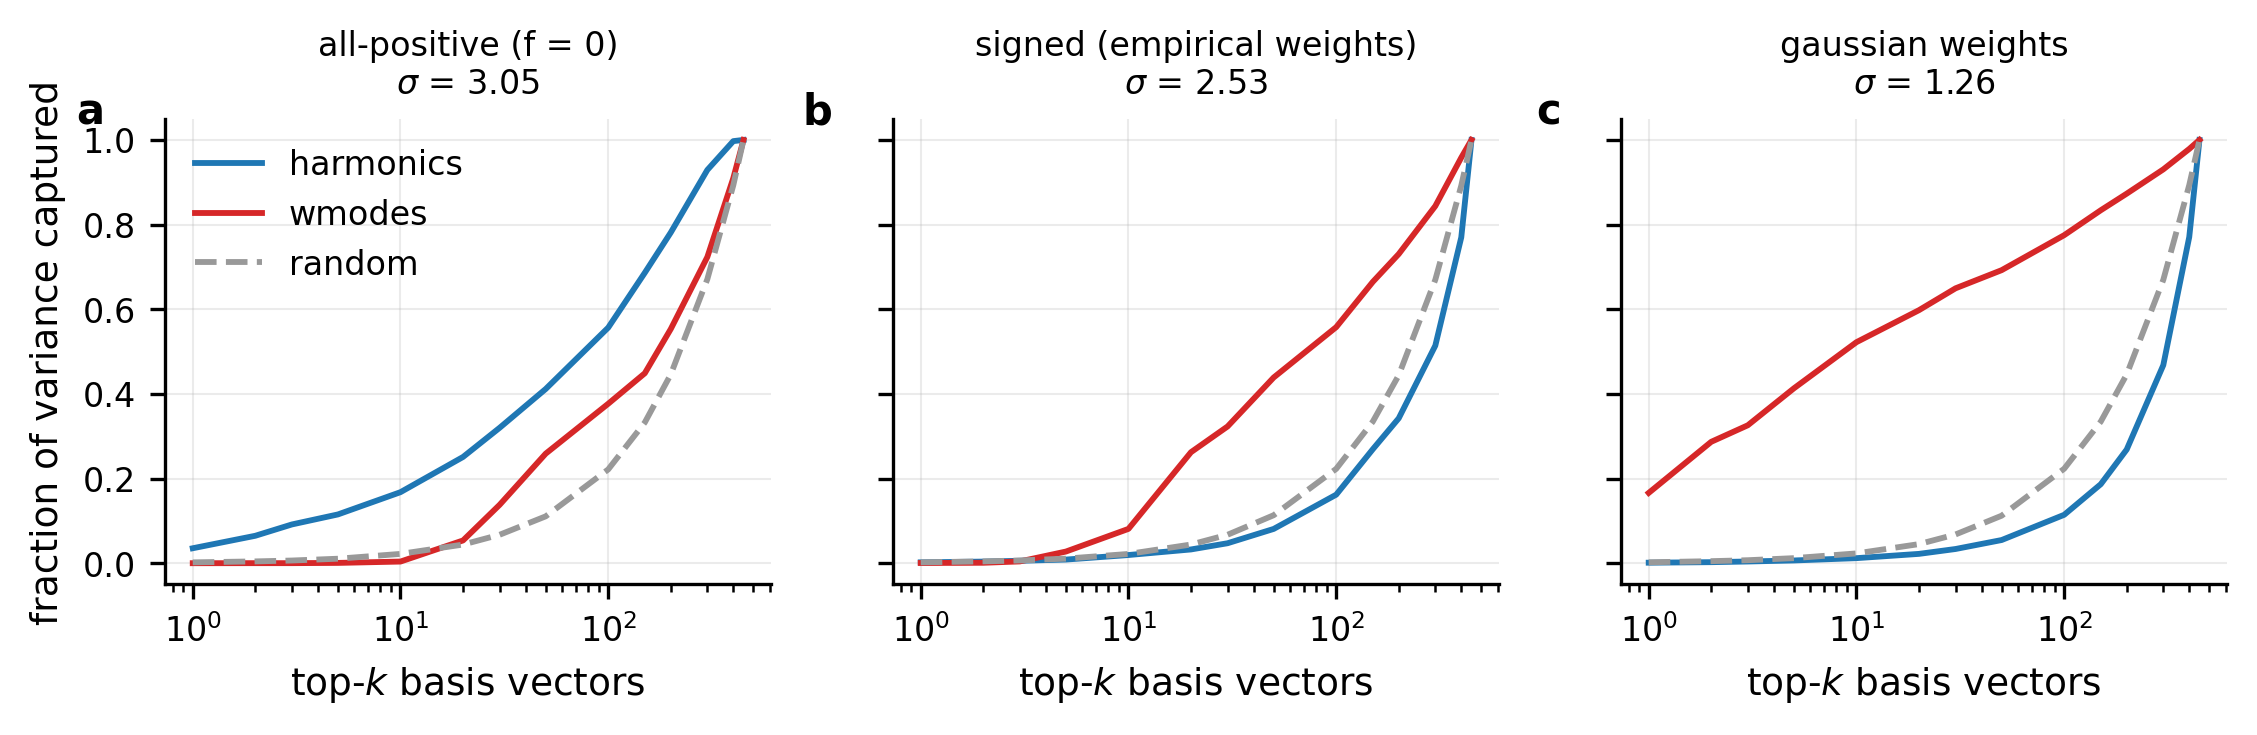
\includegraphics[width=\textwidth]{F5.png}
    \caption[Sign composition selects which structural basis the fluctuations
    occupy]{%
    \textbf{Which structural basis the fluctuations occupy is set by the weight
    signs, not by the topology.} Fraction of time-centred state variance held by
    the leading $k$ vectors of each basis, connectome substrate, Lorenz task,
    $N = 448$, % TIER0 2.1
    medians over ten seeds, each panel at its own condition's supercritical
    operating point. \textbf{(a)} With \textbf{non-negative} weights the graph
    harmonics lead throughout and the dominant $\mathbf{W}$ eigenmodes run below chance.
    \textbf{(b)} With the \textbf{same weight magnitudes} and balanced signs the
    ordering has already reversed. \textbf{(c)} With \textbf{gaussian} weights
    the eigenmodes dominate outright. The rule marks $k = 10$, where the values
    of Table~\ref{tab:app-basis} are read; the swap is visible across the whole
    curve, and the topology is identical in all three panels. On the all-positive substrate neither basis holds much in
    absolute terms; the ordering is what the panels establish. The degree-preserving rewire, the only
    other substrate this capture holds, shows the same swap at the same three
    operating points, reading
    0.168 against 0.002, % A2 F5
    0.011 against 0.102, % A2 F5
    and 0.011 against 0.355; % A2 F5
    two substrates cannot speak to the null ladder.}
    \label{fig:F5}
\end{figure}




\section{Peak memory capacity against ridge strength}
\label{app:peak-parity}
\bigskip

Section~\ref{sec:act3-memory-sigma} states parity at the peak and reports the
interval behind it. The comparison is here in full. Each substrate is taken at
its own best spectral radius and differences are paired within seed, so every
comparison shares its input weights and its input series, and the whole panel is
repeated at five ridge strengths spanning five orders of magnitude. The five are
shown because usable dimensionality tracks measured memory at
$+0.999$ % TIER0 3.3
across all of them, on the seed-median statistic over
$n = 52$; % TIER0 3.4
raising the regularisation does not break that correspondence provided it is
raised in both places at once, so the readout's regularisation is not what
produces the result in either direction.

The smallest ridge is also where this thesis meets an ordering in the literature
that appears to contradict it. Nearest the pseudoinverse limit, peak memory
orders Erdős--Rényi, degree-matching, weight-permuted, connectome, which is the
spread-beats-compact ordering of Aceituno et al.~\cite{aceituno2020tailoring}
reproduced exactly on these substrates. Section~\ref{sec:act3-memory-sigma} reads
the two results as statements about different places on the operating range: spread wins at
the peak, and a large spectral gap wins across the range.

\begin{figure}[ht]
    \centering
    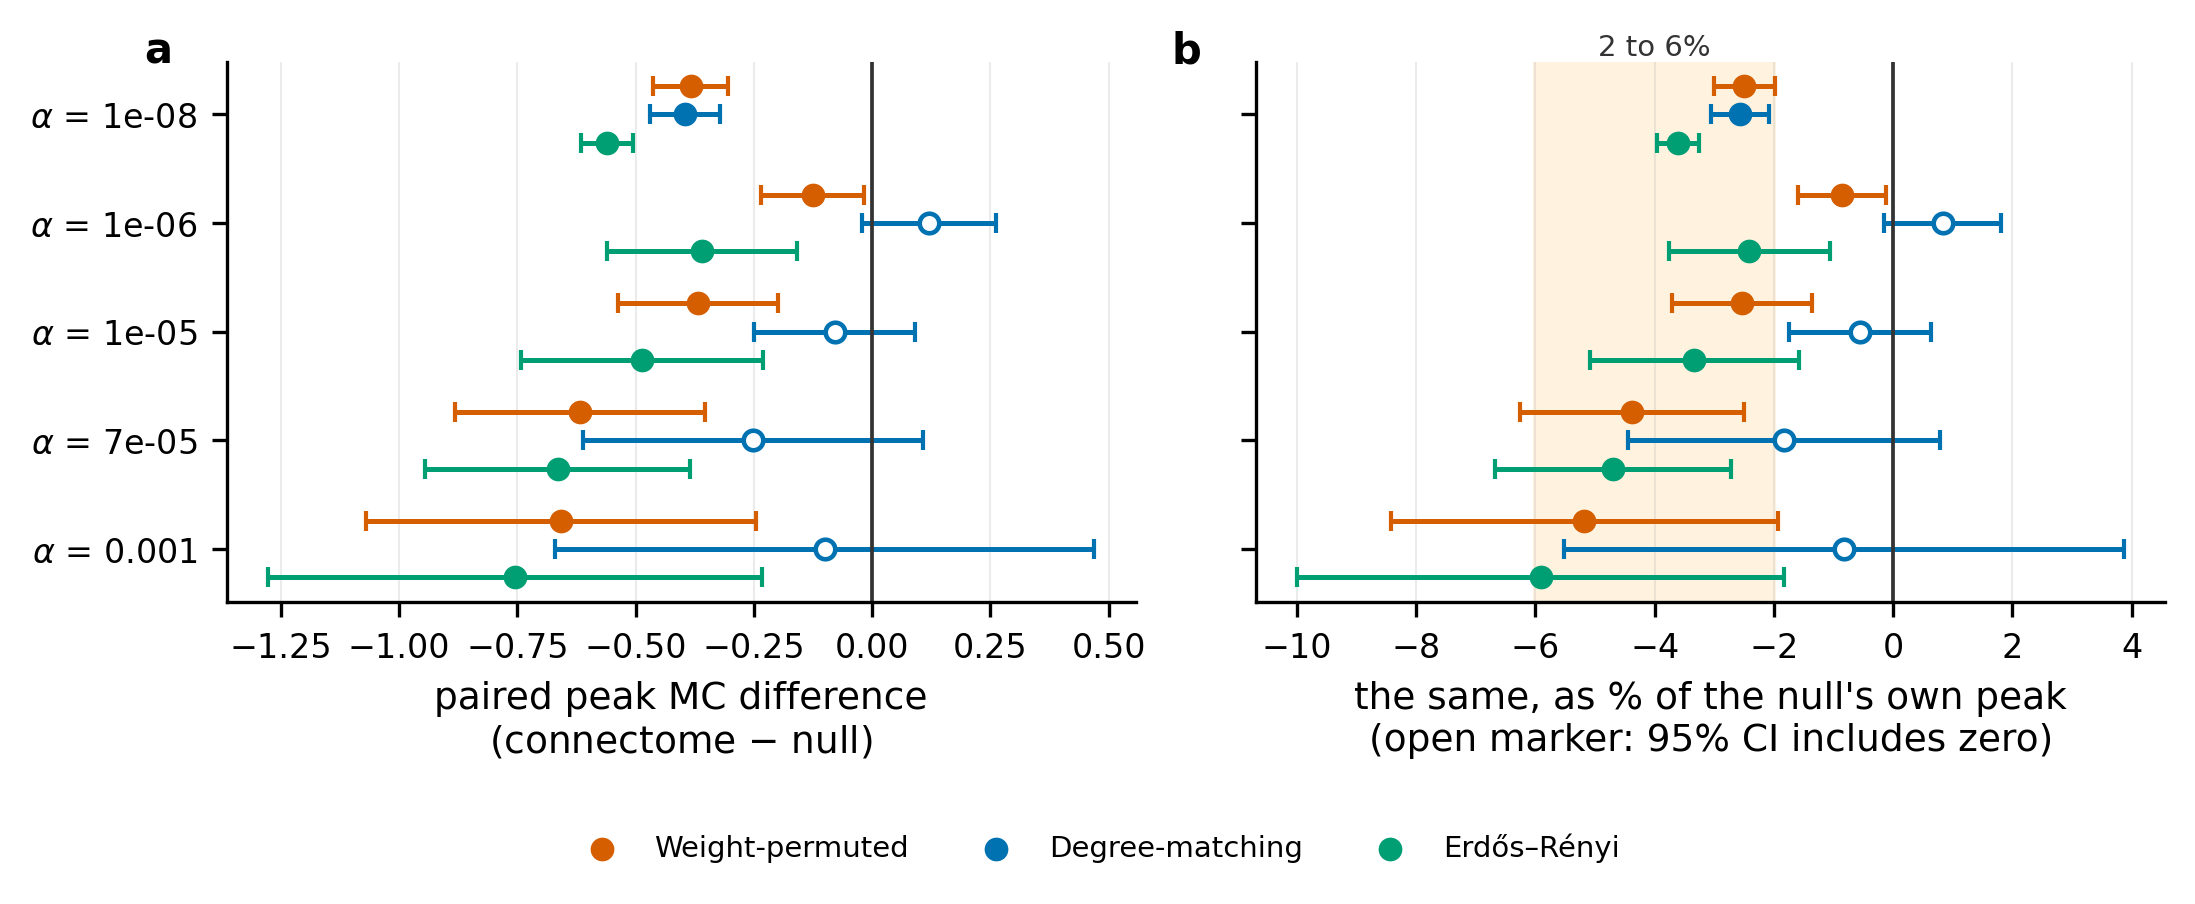
\includegraphics[width=\textwidth]{F10.png}
    \caption[At its own optimum the connectome's memory is at parity with the
    nulls]{\textbf{At its own optimum the connectome's memory is at parity with the
    nulls, not below them all.} Paired per-seed differences in peak memory capacity,
    each substrate taken at its own best spectral radius, ten seeds, with input
    weights and input series shared within a pair. Bars are $95\%$ $t$-intervals and
    filled markers are intervals excluding zero. \textbf{(a)} In memory-capacity
    units and \textbf{(b)} as a percentage of each null's own peak. The deficit is
    $2$ to $6\%$, and it excludes zero at all five ridge strengths against
    Erdős--Rényi and against the weight-permuted assignment control, but at only one
    of five against degree-matching, where the estimate also changes sign: the open
    markers. The five strengths span five orders of magnitude and are shown because
    usable dimensionality tracks measured memory at $+0.999$ across all of them
    (seed-median statistic, $n = 52$), so the readout's regularisation is not what
    produces the result.}
    \label{fig:F10}
\end{figure}



\section{The memory margin across network scale}
\label{app:scale}
\bigskip


Figure~\ref{fig:F9} reports a memory margin that holds across a 2.2-fold change in 
network size. Two things changed between the two runs, and they are separated by a 
control. The run length was scaled from
$3000$ to $6000$ % TIER0 2.5
so that the ratio of retained timesteps to units stayed near
$5.5$, % TIER0 2.5
and the ridge was reparameterised to scale with the Gram matrix rather than held
at an absolute value. At fixed $N$ the reparameterisation alone moves the
supercritical margin from
$4.35$ to $4.40$, % TIER0 2.4
so anything beyond that is attributable to size.
Two predictions stated before the run held: the margin does not vanish, and the
larger network does not escape the ceiling, peak usable dimensionality running at
$0.971$ for the connectome and $0.984$ to $0.999$ % TIER0 2.4
of its maximum for the nulls.

One thing this run was designed to settle and did not. It carried a
pre-registered falsification test, on the prediction that if the bulk radius is
what orders the ladder, then a reversal in that quantity between the two sizes
should reverse the memory ordering with it. The memory ordering did not move.
But the reversal the test rests on is itself not significant at the larger size
($p = 0.16$), % TIER0 2.4
so the test was flawed rather than passed: the correct classification is
inconclusive, and it is inconclusive because the predictor was noisy and not
because the outcome was. The registration asserted that the test was on the sign
rather than the size without first checking that the sign was established. The
question it was meant to answer is asked again in
Section~\ref{sec:act3-lesion}, by an intervention that removes the
proposed mechanism outright and therefore does not depend on a predictor moving.




\section{A second mode of generative failure}
\label{app:second-failure}
\bigskip
% Destination for chapter 6 section 6.3's zero-VPT paragraph, moved here as a
% negative result bounding A3P.4. The bounding statement stays in the main text
% beside the claim (CONVENTIONS working rule 8); the counts are here.
% NUMERALS GATED: every count below is from the read-only audit of 30 Aug as
% reproduced by verification V4 on 3 September, and is filed nowhere above rank
% 5. DO NOT SET until GAPS B26 is committed. Unit: the seed-cell,
% 1160 = 4 variants x 29 sigma x 10 seeds, three draws collapsed because at
% f = 0 the sign transform is the identity.
% The reason chapter 6 previously gave for separating the two modes is
% WITHDRAWN: the collapse flag IS persisted per seed and draw, and the two can
% be matched. See V4.
% FORBIDDEN: reading the two modes as one event; "50% of replicates".

Section~\ref{sec:act3-prediction-sigma} reports that the connectome alone avoids
the period-two collapse, and bounds that result with a second and cruder measure
on which the ordering reverses. Counting seeds that record a valid prediction
time of exactly zero at any operating point, the connectome has
five of ten, % GAPS B26
the weight-permuted control
three, % GAPS B26
Erdős--Rényi
two, % GAPS B26
and the degree-matched null none at all, its lowest value anywhere in the sweep
being
$0.068$. % GAPS B26

Three things bound how much should be read into that. The failures are confined
to the upper sweep, the lowest operating point at which any connectome seed
records a zero being
$\sigma = 3.6$, % GAPS B26
so none occurs at or below the point at which the near-critical comparison of
Section~\ref{sec:act3-prediction-sigma} is made. They are never a whole
condition failing: at worst half the seeds of a condition score zero while the
rest predict at between one and three Lyapunov times, in line with their
neighbours. And they are a different event from the collapse rather than a
milder form of it, which can now be shown rather than assumed. Both flags are
recorded per seed, so the forty seeds at zero sign fraction cross-tabulate
directly:

\begin{center}
\begin{tabular}{lcc}
    \toprule
    & \multicolumn{2}{c}{zero prediction time} \\
    \cmidrule(lr){2-3}
    collapses to period two & no & yes \\
    \midrule
    no  & $25$ & $6$ \\
    yes & $5$  & $4$ \\
    \bottomrule
\end{tabular}
\end{center}

All five of the connectome's zero-scoring seeds sit in the upper-left and
upper-right cells, since it has no collapsing seed at all; Erdős--Rényi's two
are both collapsing seeds. The two failure modes are therefore distinct, they
order the substrates differently, and both orderings are correct measurements of
different things.


\section{Regime gating against graded geometry}
\label{app:regime-gating}
\bigskip

Section~\ref{sec:act3-branch} states that predictive capacity is gated by which
dynamical regime a network occupies rather than graded by how curved its
trajectory is. The comparison behind that statement is here.

Across the full sweep in operating point and sign fraction, a single binary
variable recording which curvature spike a cell belongs to explains
$R^2 = 0.364$ % TIER0 3.10
of the variance in valid prediction time. The full continuous curvature measure
explains
$0.370$. % TIER0 3.10
The entire range of geometries lying between the two regimes is therefore worth
less than one percentage point beyond the bit, and the bit is what the
relationship consists of.

The graded account it replaces is not a straw man but an earlier reading of these
same data. Pooled across all cells, curvature and prediction correlate at
$-0.78$, % TIER0 3.10
which reads as a relationship in which capacity tracks how straight the manifold
is. It is cluster mixing. Within the smooth cluster alone the residual
correlation is
$+0.145$, % TIER0 3.10
opposite in sign, and no binning of the data recovers a graded path between the
clusters. The pooled figure measures the separation between two groups and not a
trend within either.




\section{Attractor retention in long rollouts}
\label{app:long-rollout}
\bigskip

Valid prediction time is measured over short rollout windows and scores how long
a released network stays with the true trajectory before leaving it. A longer
question is whether a network left running on its own output continues to
produce the right kind of trajectory at all, which is measured over a rollout of
$3000$ % A3P 2.6
steps with the first
$500$ % A3P 2.6
discarded as settling, some
$67.9$ % A3P 2.6
Lyapunov times scored, and reported as a rate over cells rather than per cell
(Section~\ref{sec:methods-closed-loop}). This section reports that measurement.

A pre-registration written before the code existed made two claims about the
long rollout: that the connectome would retain the true attractor's statistics to
a higher sign fraction than the nulls, and that when substrates failed they would
fail by distorting the attractor's shape while preserving its scale.

The first is confirmed. Once a third of the weights are negative the connectome
holds a faithful climate in
$0.43$ % A3P 6.1
of cells against the nulls'
$0.14$, % A3P 6.1
about three times the rate (Figure~\ref{fig:F17}).

The second is refuted, and the refutation is the more informative result. The
ratio of the free run's spread to the true trajectory's spread is sharply
bimodal, with cells either collapsing below a twentieth of it or holding within a
tenth of unity and almost none between. A failed rollout is therefore a collapse
of scale and not a distortion of shape, which is the fixed-point branch of the
map of Section~\ref{sec:act3-branch} seen in the closed loop, on a different
quantity and a different capture from anything in that chapter.

\begin{figure}[htbp]
    \centering
    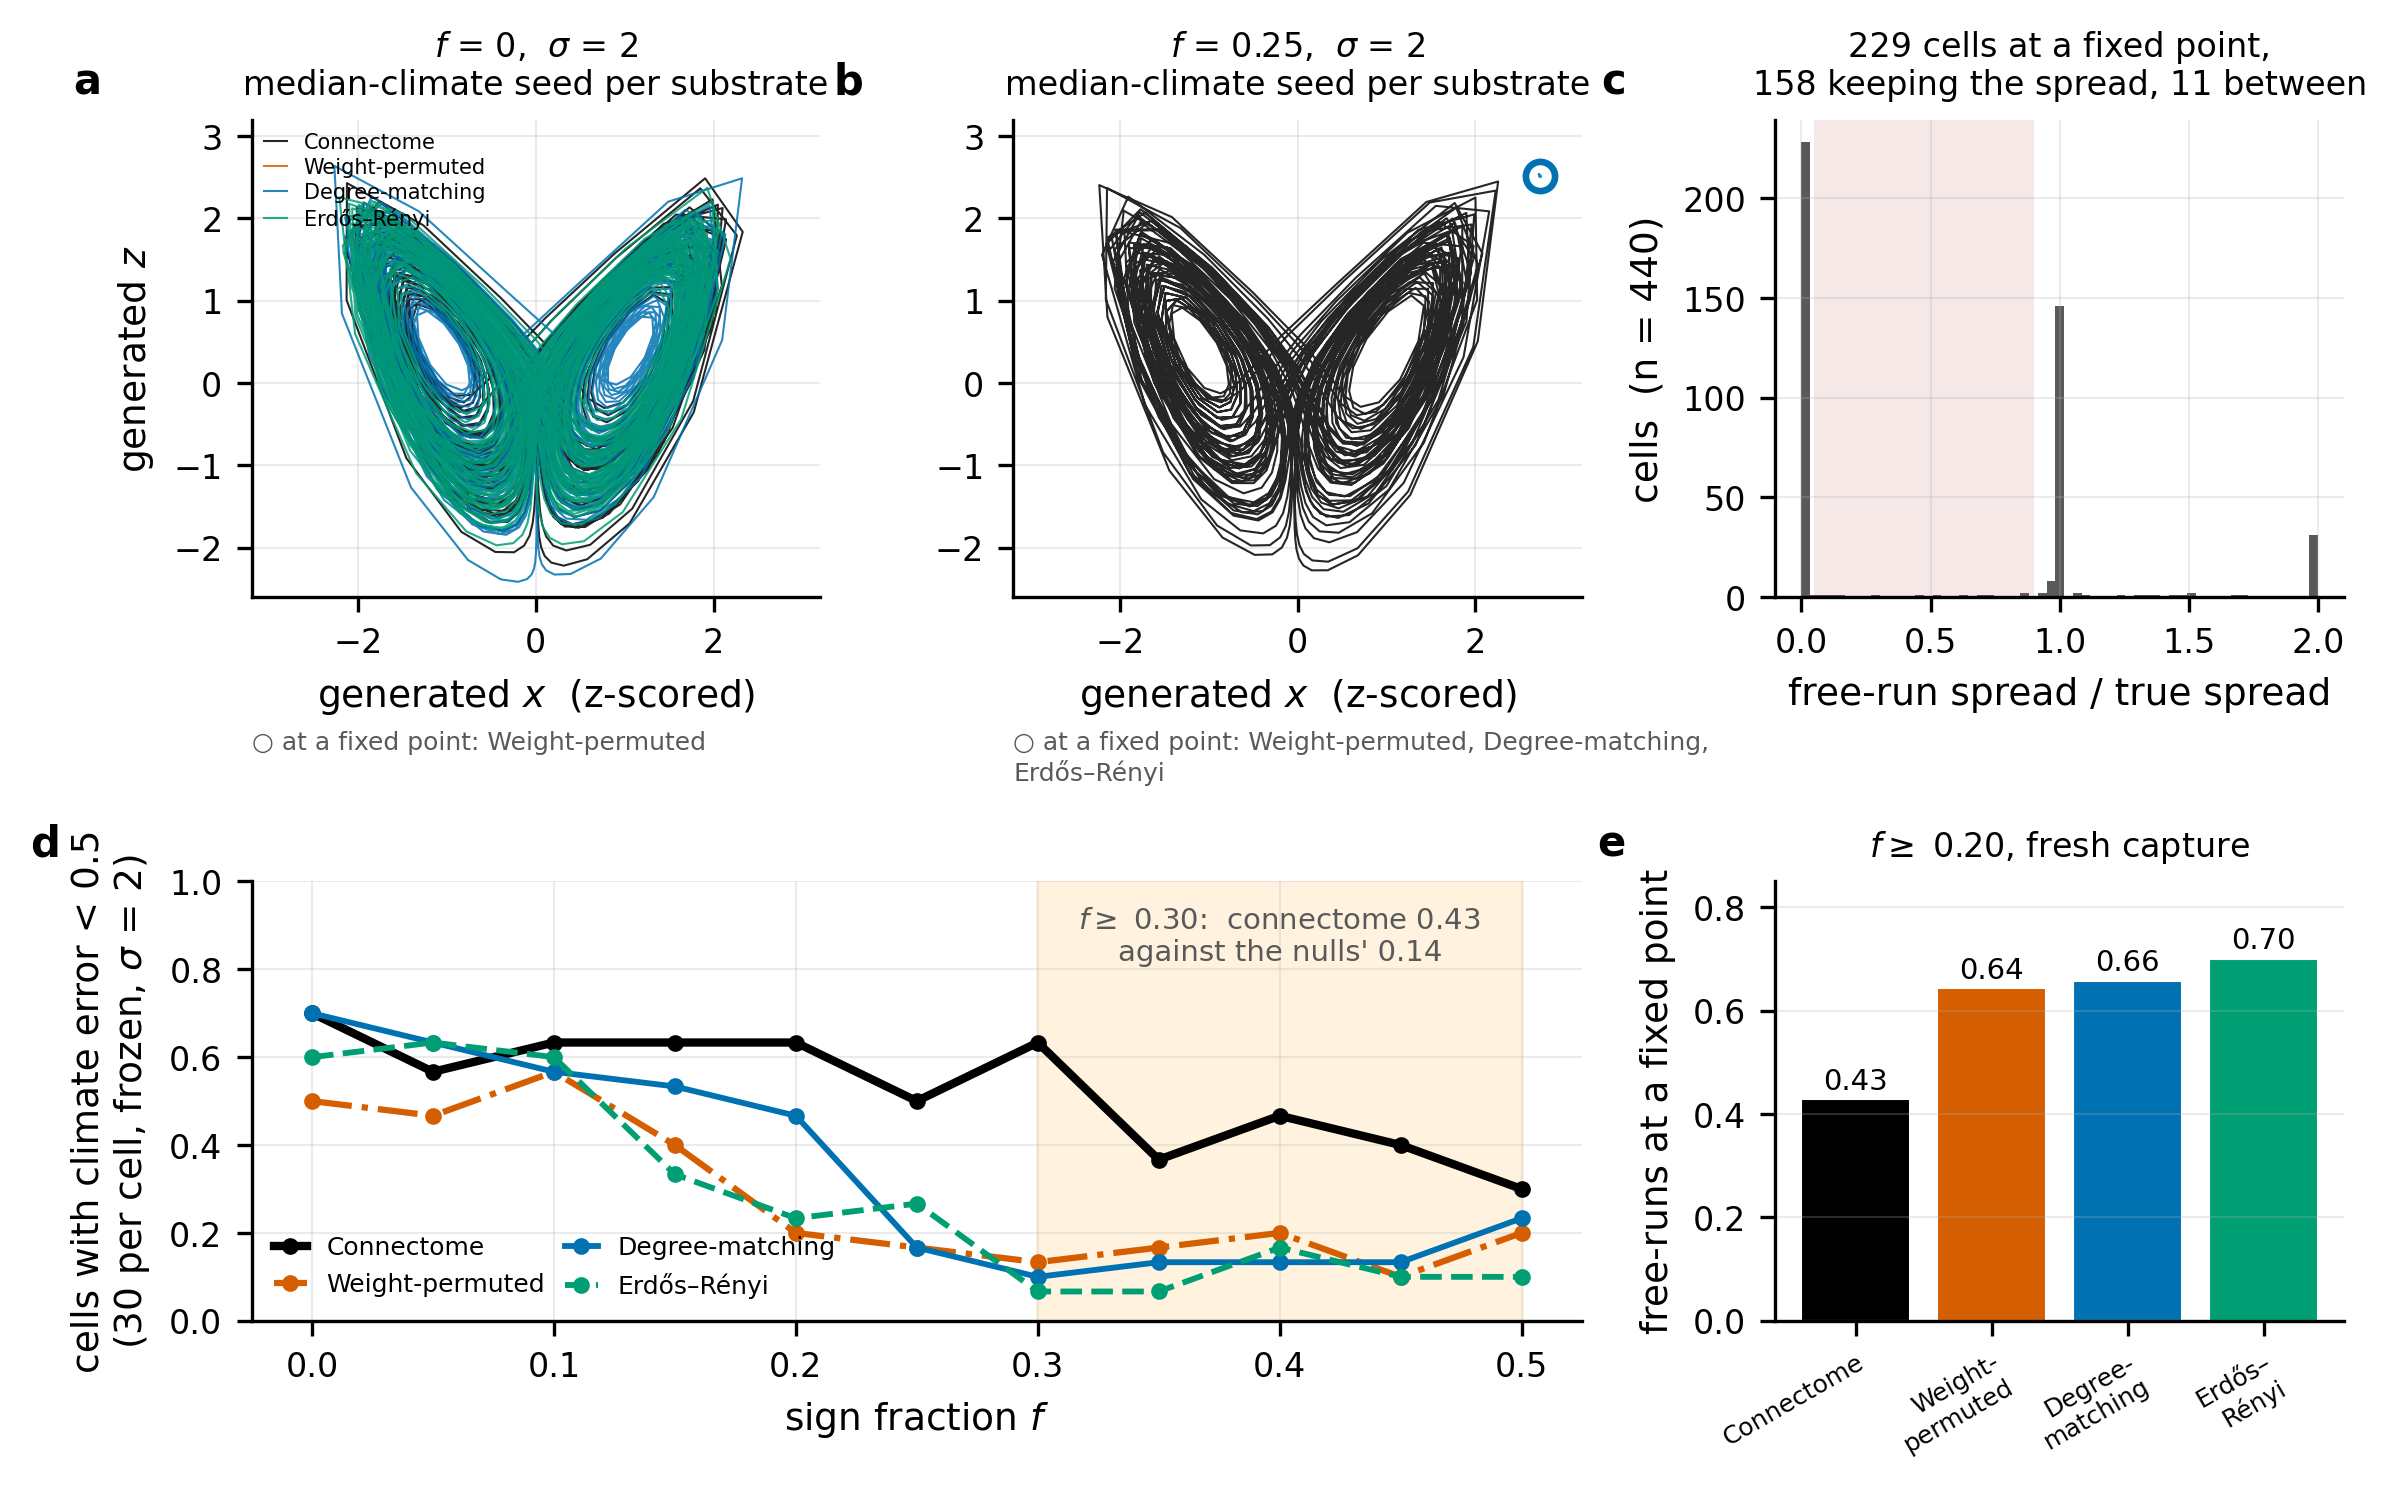
\includegraphics[width=\textwidth]{F17.png}
    \caption[Released to run alone, the connectome holds the true attractor
    further, and failure is a collapse of scale]{\textbf{Released to run alone,
    the connectome holds the true attractor further, and failure is a collapse of
    scale.} Free-running Lorenz rollout, $N = 448$, at $\sigma = 2$, against the
    sign fraction $f$. \textbf{(a, b)} Example rollouts either side of the
    separation. \textbf{(c)} The ratio of free-run spread to true spread, which
    refutes the second registered claim: of $440$ cells, $229$ fall below $0.05$
    and $158$ lie within a tenth of unity, with $11$ between, so failure is a
    loss of scale rather than a distorted shape. The registered description,
    wrong shape at right scale, fits $34$ cells. \textbf{(d)} The fraction of
    cells whose free run keeps the true attractor's statistics, confirming the
    first registered claim. \textbf{(e)} Where collapsed rollouts come to rest,
    most of them several z-scored units from the origin, against an attractor
    spanning about $\pm 2.5$ per coordinate. Panel (a) is read from the frozen
    capture and the rate in the text from a separate fresh capture; the two are
    not one population and are not combined.}
    \label{fig:F17}
\end{figure}



% ------------------------------

% S1
\begin{figure}[ht]
    \centering
    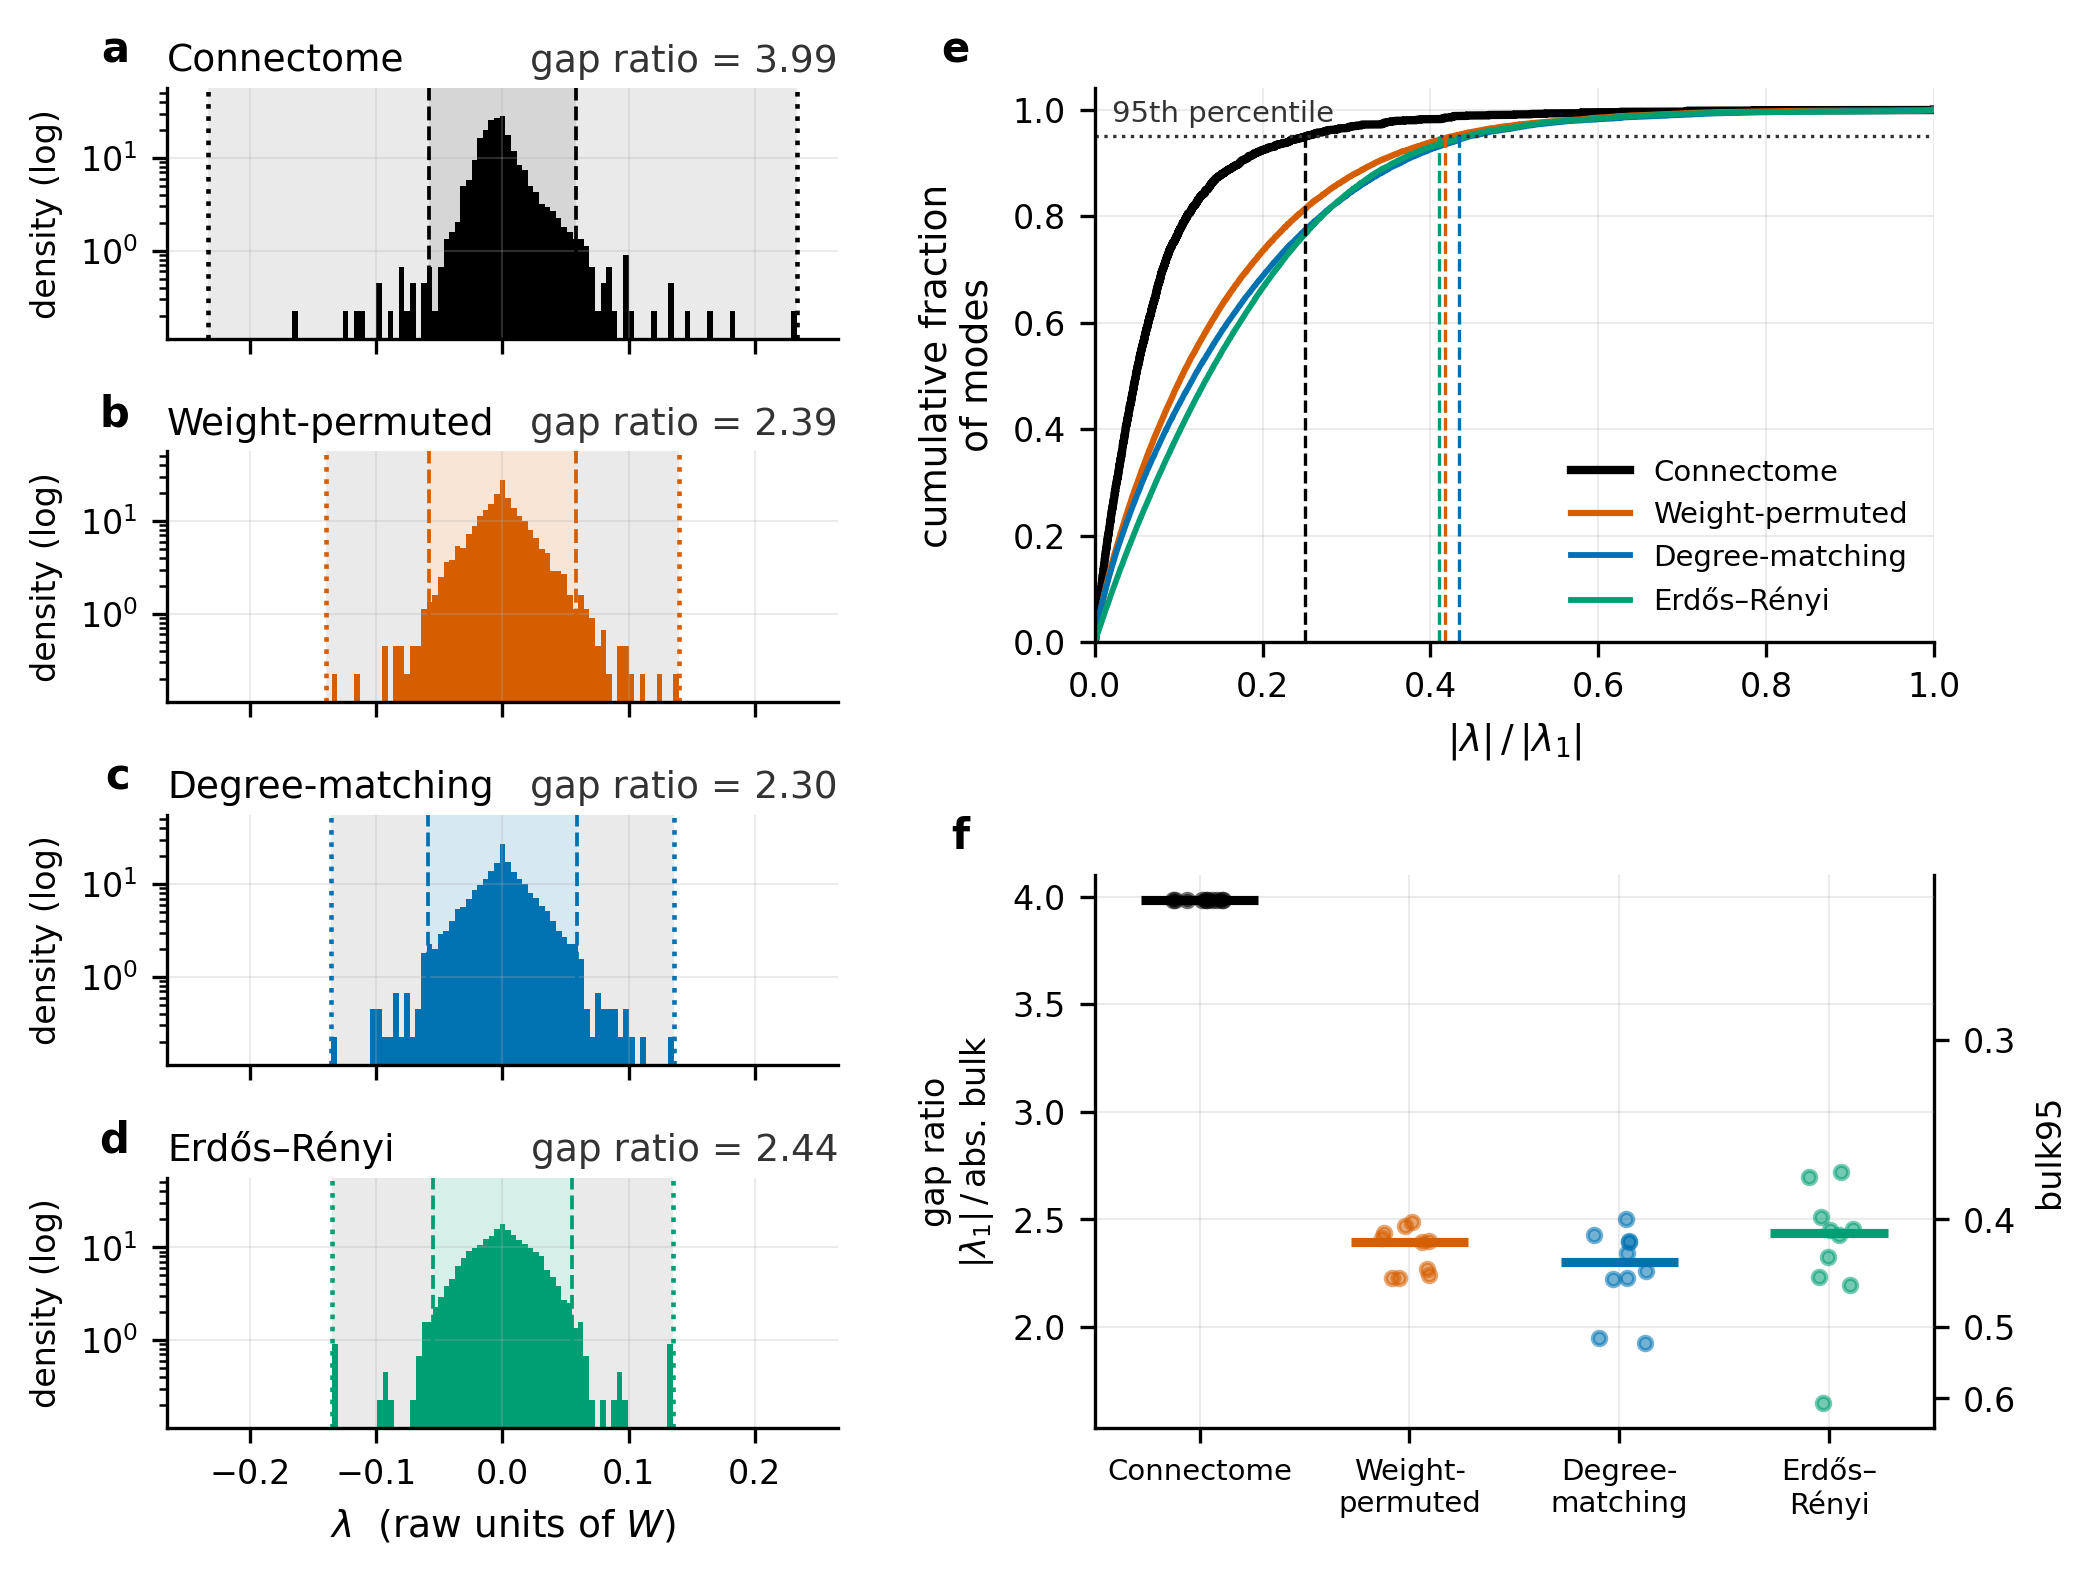
\includegraphics[width=\textwidth]{S1.png}
    \caption[Figure~\ref{fig:F1} rebuilt at the larger parcellation]{
    \textbf{The spectral gap at $N = 1000$.} As Figure~\ref{fig:F1} in every
    respect, same substrate family, same null ladder and same builder, at the
    $N = 1000$ % TIER0 2.1
    self-built consensus. \textbf{(a--d)} The four bulk bands again sit at the
    same place while $\lambda_1$ separates, and the connectome's gap ratio again
    stands at least 1.63-fold % TIER0 3.1(b)
    clear of every rung of the four-substrate ladder, 3.99 % TIER0 3.1
    against 2.30 to 2.44. % TIER0 3.1
    The rows are in ladder order and their gap ratios are \emph{not} monotone
    here, reading 3.99, 2.39, 2.30 and 2.44 % A1 S1 caption
    down the column, because the ordering of the three nulls by
    $\mathrm{bulk95}$ reverses between the two parcellations. What is
    scale-robust is the connectome's separation from the nulls, not the
    arrangement among them, and not the near-identity of the bulks, whose spread
    loosens from 4.4\% at $N = 448$ % TIER0 3.1
    to 6.4\% here, on the product of the medians. % TIER0 3.1
    \textbf{(e)} $\mathrm{bulk95}$ read off the 95\% crossing:
    0.251 % A1 S1 caption
    against 0.410 to 0.435. % A1 S1 caption
    \textbf{(f)} The per-seed gap ratio; the connectome's ten seeds again
    coincide exactly.}
    \label{fig:S1}
\end{figure}

    \chapter{Appendix: Data Availability}
\label{appendix:data}


    \chapter{Appendix: Code Availability}
\label{appendix:code}



    
    
\end{document}
